\documentclass{article}
\usepackage{graphicx} % Required for inserting images

\title{\Huge FROZEN LAKE'S REINFORCEMENT LEARNING AGENT REPORT}
\author{Francesco Saverio Sconocchia Pisoni 1889241}
\date{March 2025}

    


\begin{document}

\maketitle

\begin{center}
    \centering
    \resizebox{\textwidth}{!}{
\includegraphics{logo Sapienza (rgb).png}}
\end{center}

\section*{\centering ARTIFICIAL INTELLIGENCE AND MACHINE LEARNING 2023/2024}
\clearpage


\section{Introduction}

This machine learning project aims to maximize the average reward taken by solving the Frozen Lake environment, using reinforcement learning techniques.
This technique allows us to reach the goal through a slippery (in this case) obstacle path.
This is done by creating an agent which interfaces with this environment (through the Gymnasium library), collecting a reward and arriving to a new reached state.
The agent is able to calculate and improve an expected reward by taking an action in a state, using the non-deterministic Q-learning method.
After the calculated Q-table is converged to an optimal solution, the agent could solve the environment by choosing the best expected reward action from the Q-table itself.

\begin{center}
\centering
\resizebox{\textwidth}{!}{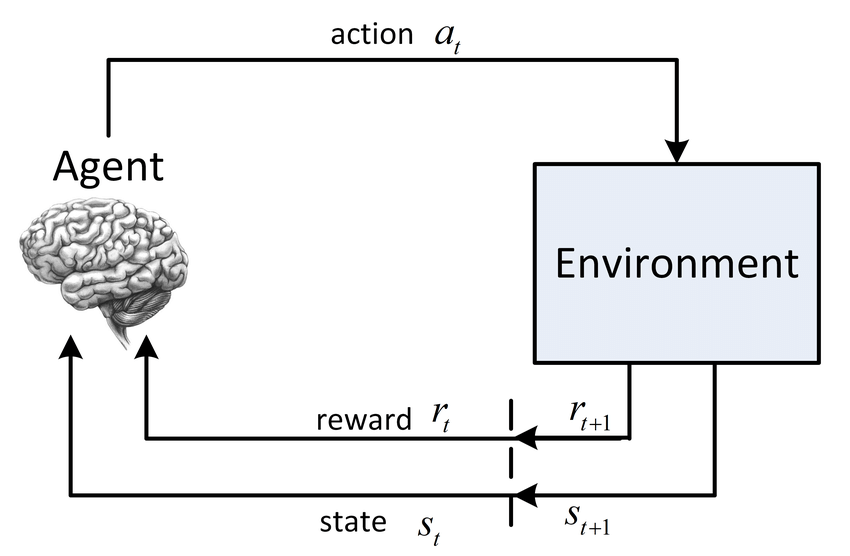
\includegraphics{agent-environment-schema.png}}
\end{center}

We use the non-deterministic method, because of the slippery of the floor of the environment, which could bring (with a certain probability) the agent to find itself in a non-expected state, after performing a chosen action.

The non-deterministic Q-learning method is described below:

\begin{center}
\centering
\resizebox{\textwidth}{!}{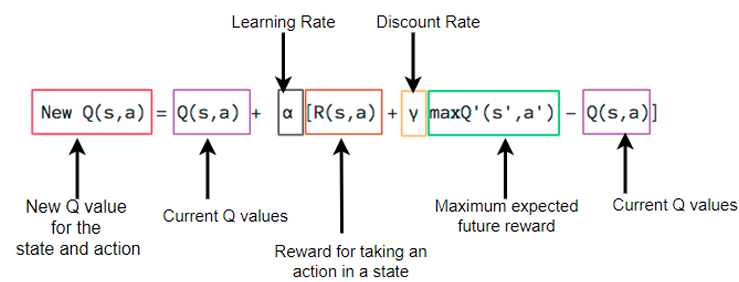
\includegraphics{nd-Q-learning-function.png}}
\end{center}

Is needed to clarify the meaning of those parameters:

\begin{itemize}
\item[--]{Learning rate $\alpha$: it indicates how fast should change the Q-table's parameters in the training phase}
\item[--]{Discount rate $\gamma$: it determines the importance of future rewards}
\item[--] {max Q'(s', a') : it calculates the maximum Q-value among all the possible actions which could be taken from the new reached state s'}
\end{itemize}


\section{Environment}

The Frozen Lake environment has the following characteristics: 
\begin{itemize}
\item[--]{An observation space of 16 possible values, where each possible integer indicates a specific cell of the map, which is the player’s current position and is calculated as current\_row * ncols + current\_col}
\item[--] An action space of 4 possible values, representing the following actions: 0 = Move left, 1 = Move down, 2 = Move right, 3 = Move up
\item[--] The reward could be 1 if the agent reaches the goal, or 0 if not
\item[--] Each episode terminates if the agent reaches the goal or if the agent hits an obstacle (falls in the lake) or if the agent performs more than 100 steps in an episode
\item[--] The slippery characteristic is encoded in this way: the player will move in intended direction with probability of 1/3 else will move in either perpendicular direction with equal probability of 1/3 in both directions.
\end{itemize}

\subsection{Exploration-exploitation}

When the agent, in the training phase, has to choose an action to perform in order to improve its Q-table, we want that it chooses primarily random actions in order to better exploring all the environment and its rewards.
But later on, we want to converge to an optimal solution, which could be reached by using the best actions to be able to achieve the goal.


\subsection{General solution adopted}


My solution for both Deep Q Network and Tabular Q Learning methodologies used for solving the environment uses:
\begin{itemize}
\item[--] The Epsilon-greedy strategy : Is chosen either the best action with a probability 1-$\epsilon$ or a random action in the training phase, for managing the duality exploration-exploitation.
\item[--] The epsilon $\epsilon$ parameter decreases linearly with a decay factor, until reaches a minimum value, so achieving first exploration and then exploitation.
\end{itemize}

\section{Map 4x4}



\section{Tabular Q Learning}

\subsection{Solution adopted}

The agent algorithm has the following characteristics:
\begin{itemize}
\item[--] {A decay function which is called at each episode for decreasing the $\epsilon$ value:
\begin{verbatim}
self.epsilon = max(self.final_epsilon, self.epsilon - self.epsilon_decay)
\end{verbatim}
}
\item[--] In the training phase, a number of episodes of 15.000 episodes
\item[--] In the training phase, a range of 250 episodes for calculating the average cumulative reward over that range of episodes, so limiting the noise
\item[--] In the test phase, a number of 500 episodes
\end{itemize}

\subsection{Metric results}

\subsubsection{Changing the epsilon decay}

These are the common hyper parameters for the runs:
\begin{itemize}
\item[--] $\alpha$= 0.1
\item[--] initial $\epsilon$ = 1
\item[--] final $\epsilon$ = 0.05
\item[--] gamma = 0.99
\end{itemize}

From the first plot to the third, the $\epsilon$ decay rate is increased as follows:
\begin{itemize}
\item[--] The first brings $\epsilon$ to its minimum value at 7/8 of the episodes.
\item[--] The second brings $\epsilon$ to the minimum at 3/4 of the episodes.
\item[--] The last one brings $\epsilon$ to the minimum at 1/2 of the total episodes.
\end{itemize}

\begin{center}
\centering
\resizebox{\textwidth}{!}{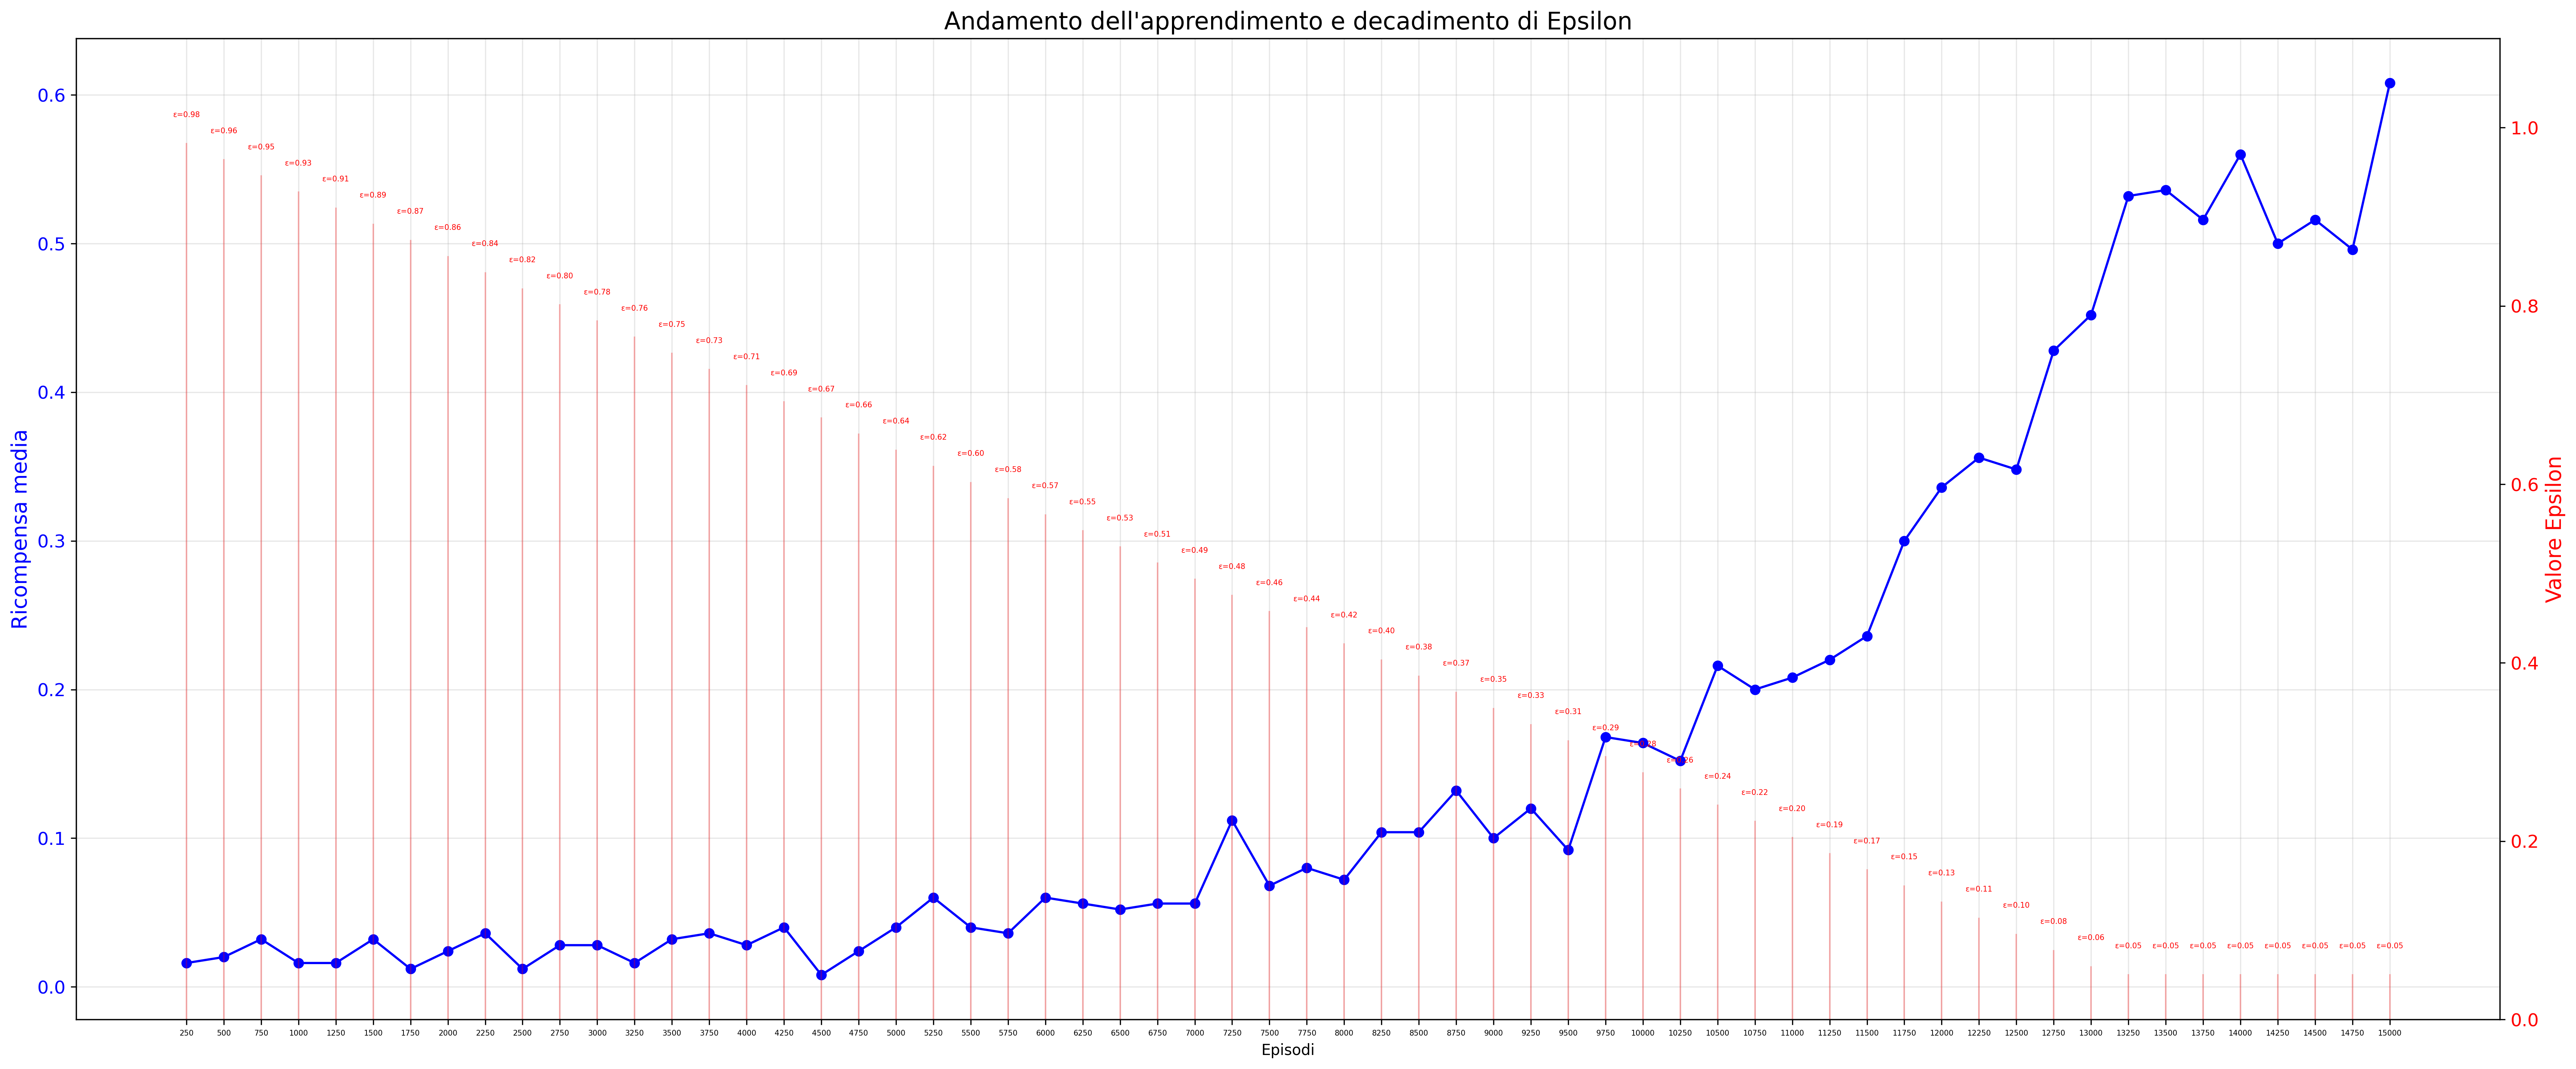
\includegraphics{TQL;lr=0.1;nep=15000;eps=1.0;fineps=0.05;eps_dec=7.238095238095238e-05;gam=0.99.png}}
\end{center}


\begin{center}
\centering
\resizebox{\textwidth}{!}{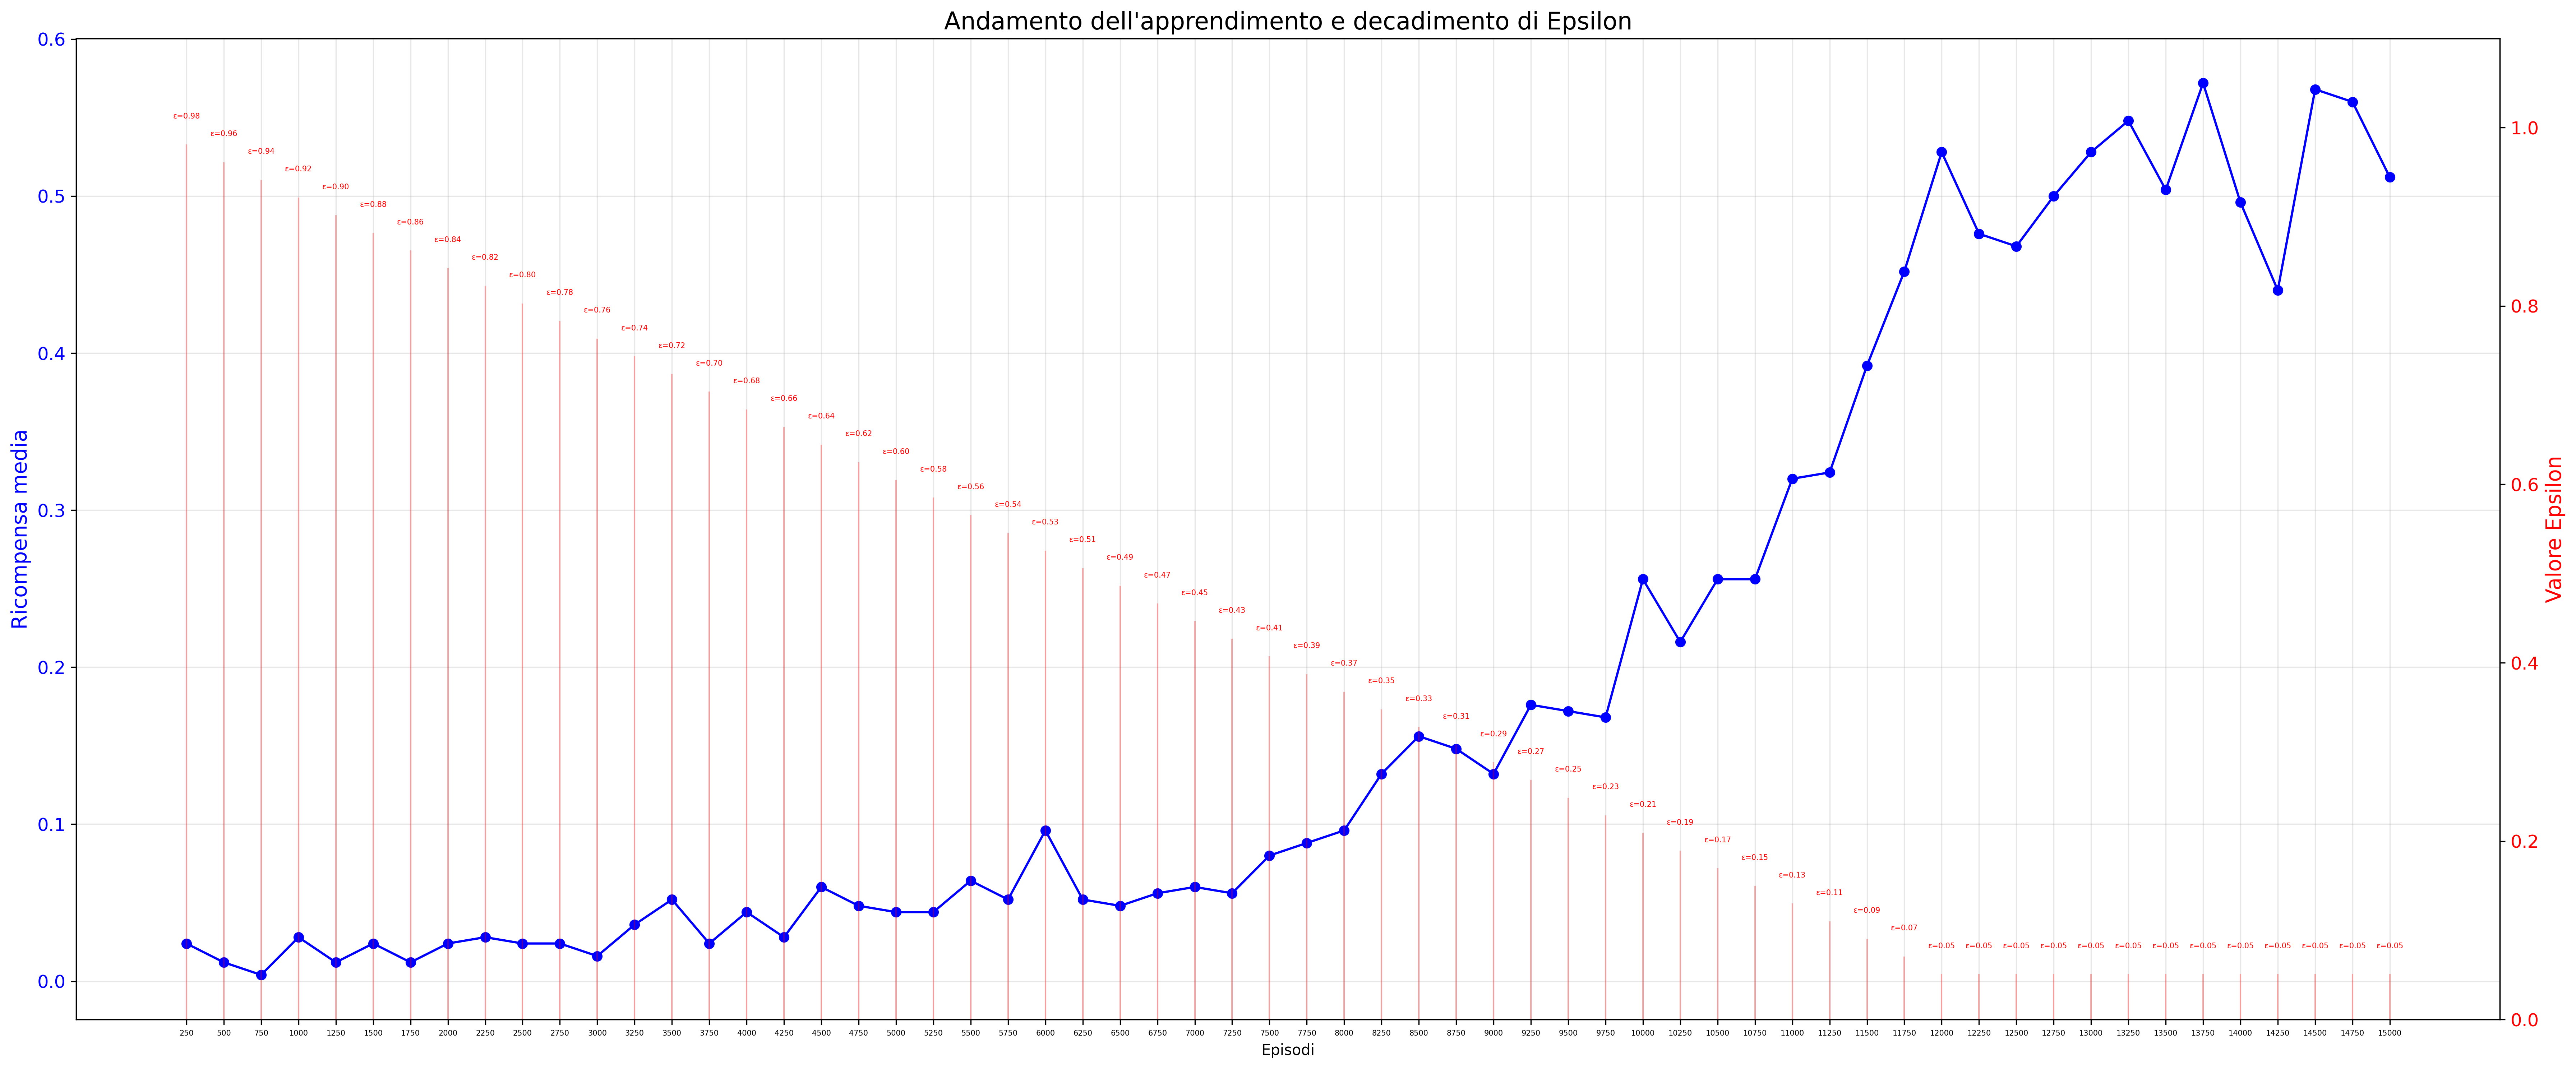
\includegraphics{TQL;lr=0.1;nep=15000;eps=1.0;fineps=0.05;eps_dec=7.916666666666666e-05;gam=0.99.png}}
\end{center}


\begin{center}
\centering
\resizebox{\textwidth}{!}{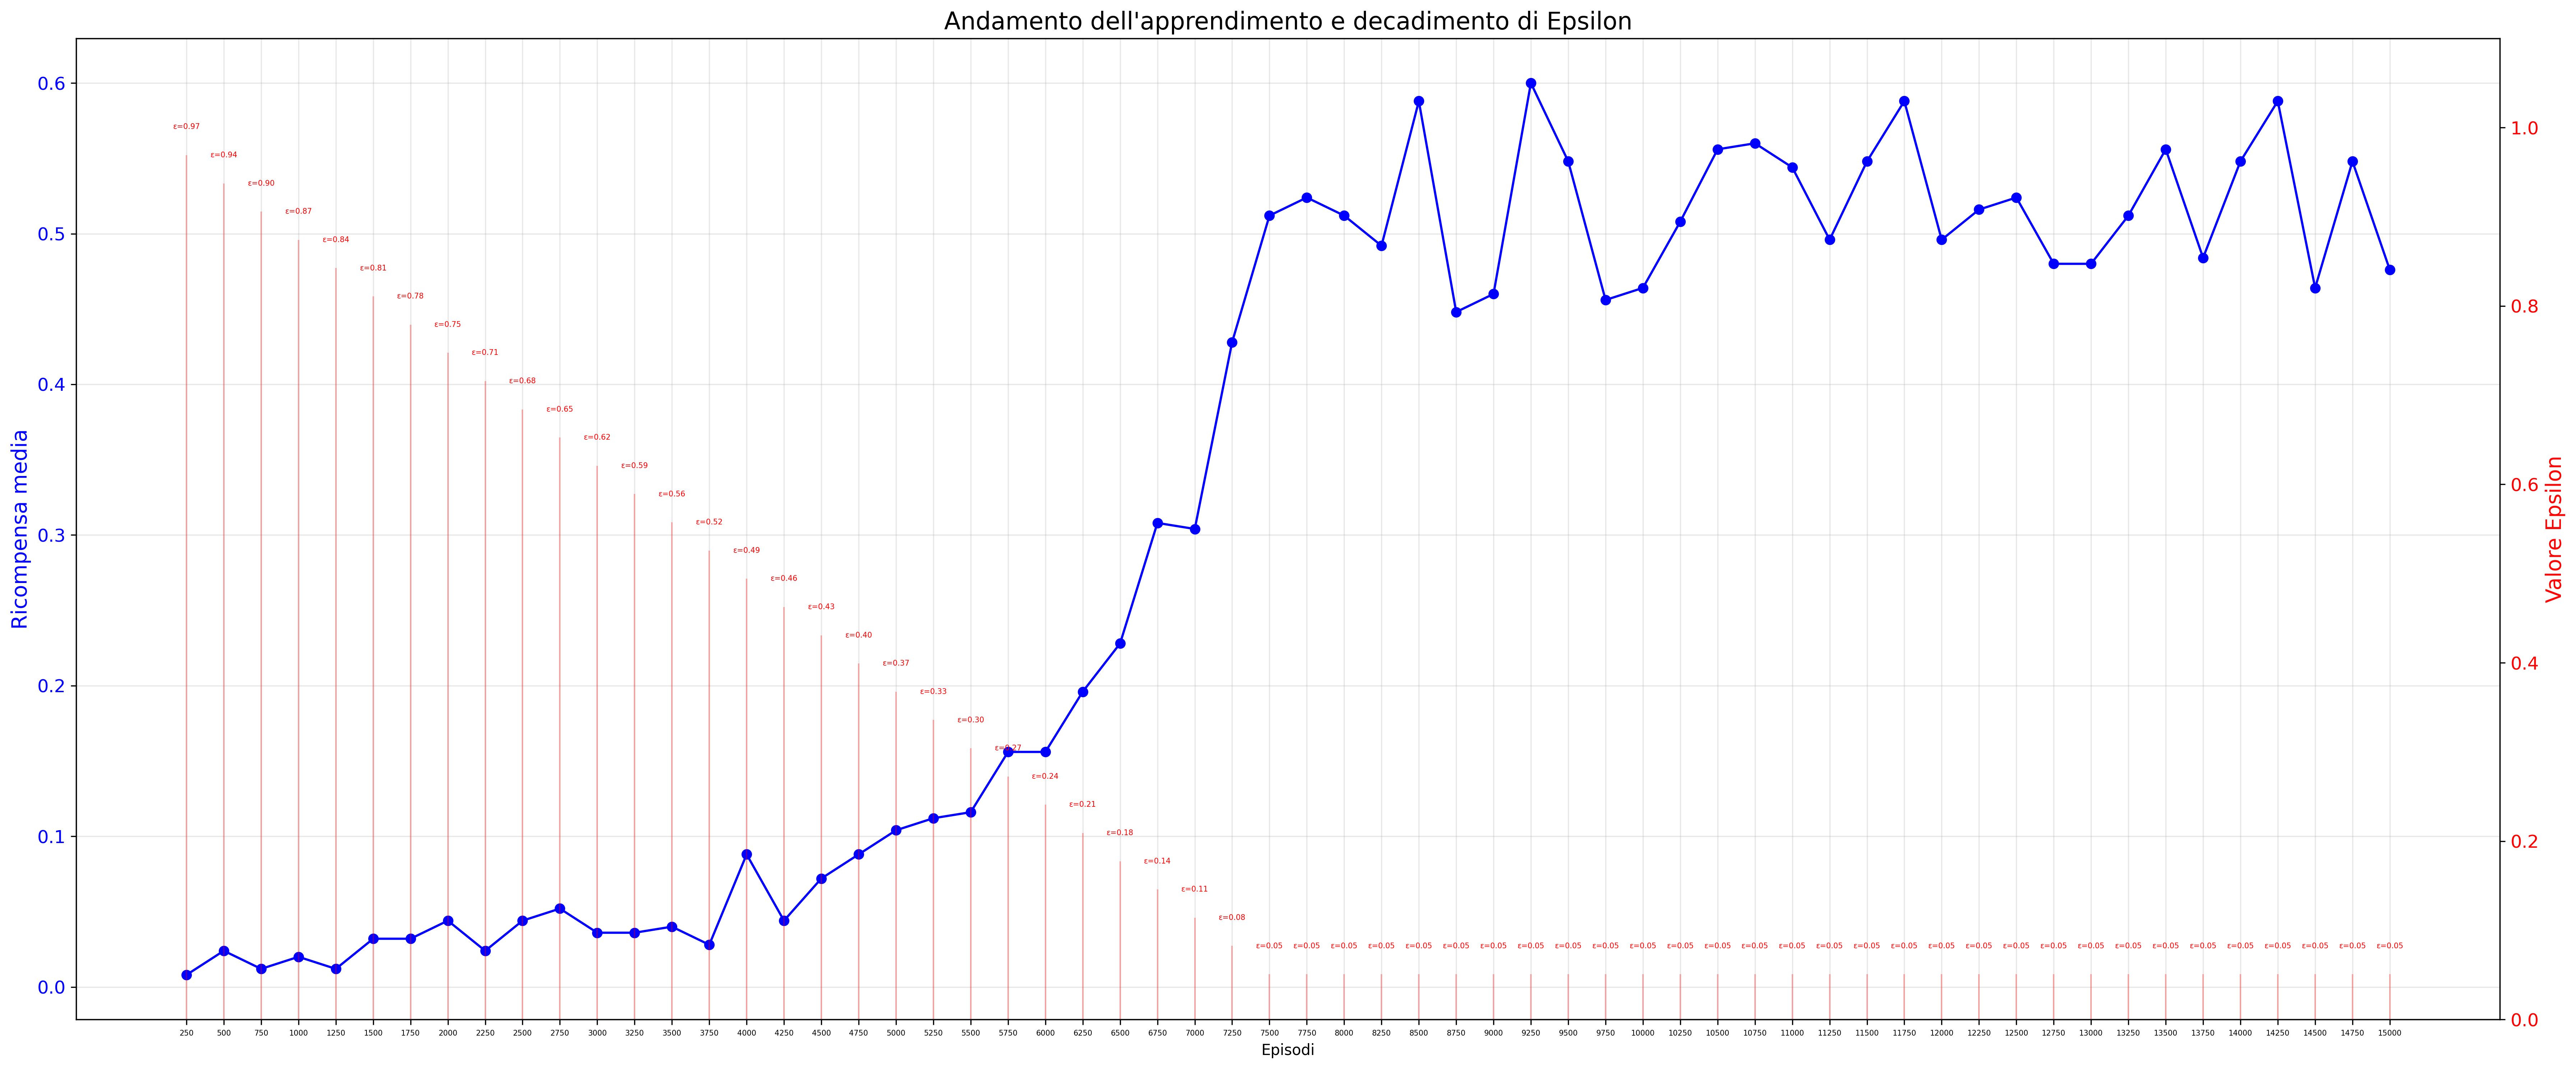
\includegraphics{TQL;lr=0.1;nep=15000;eps=1.0;fineps=0.05;eps_dec=0.00012666666666666666;gam=0.99.png}}
\end{center}

\clearpage


The convergence occurs when $\epsilon$ reaches the minimum value (0.05), so the third setting beats the others in terms of convergence time.
\\
In terms of average cumulative reward at convergence, both the first and the third configurations have roughly the same value (about 55\% success rate). Instead, the second configuration (full exploration at 3/4 of the episodes) results in an average cumulative reward of about 50\%.
\\
During the testing phase, the first configuration achieves a success rate of 73.6\% (over 500 test episodes), while the other two configurations show success rates of 72.8\% for the second one and 72.6\% for the third.
\\
Therefore, we can conclude that the third configuration is the best, due to its faster convergence time, along with one of the best average cumulative rewards at convergence and nearly the same success rate in the test phase as the other configurations.


\subsubsection{Changing the learning rate}

These are the common hyper parameters for the runs:
\begin{itemize}
\item[--] $\epsilon$ decay= 0.000126
\item[--] initial $\epsilon$ = 1
\item[--] final $\epsilon$ = 0.05
\item[--] gamma = 0.99
\end{itemize}

From the first plot to the third, the $\alpha$ value assumes the following values :
\begin{itemize}
\item[--] The first sets $\alpha$ to 0.1
\item[--] The second sets $\alpha$ to 0.01
\item[--] The third sets $\alpha$ to 0.001
\end{itemize}

\clearpage


\begin{center}
\centering
\resizebox{\textwidth}{!}{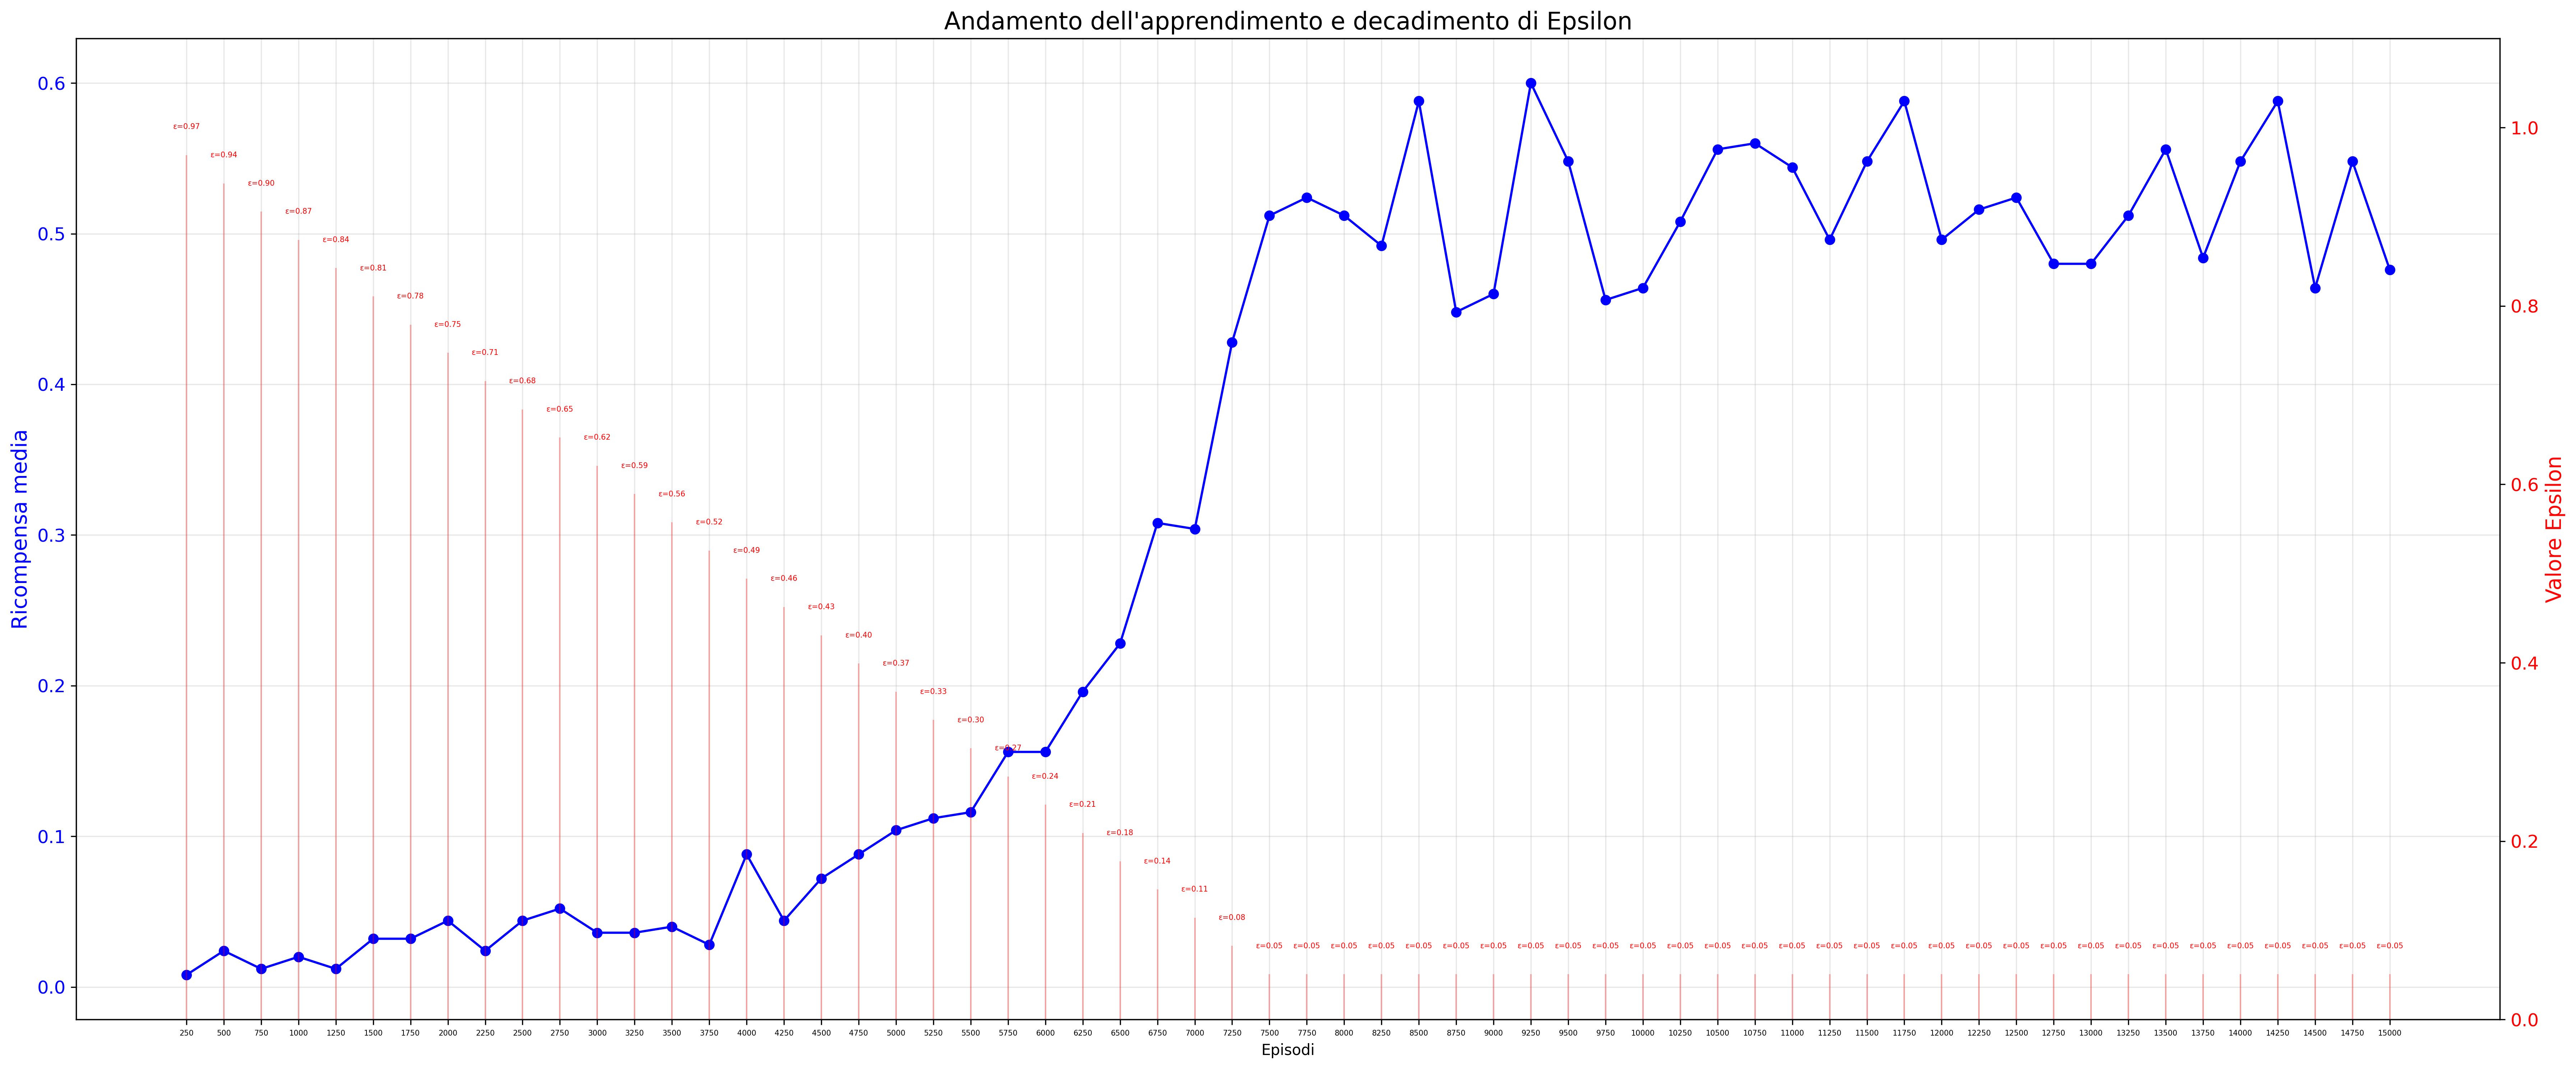
\includegraphics{TQL;lr=0.1;nep=15000;eps=1.0;fineps=0.05;eps_dec=0.00012666666666666666;gam=0.99.png}}
\end{center}

\begin{center}
\centering
\resizebox{\textwidth}{!}{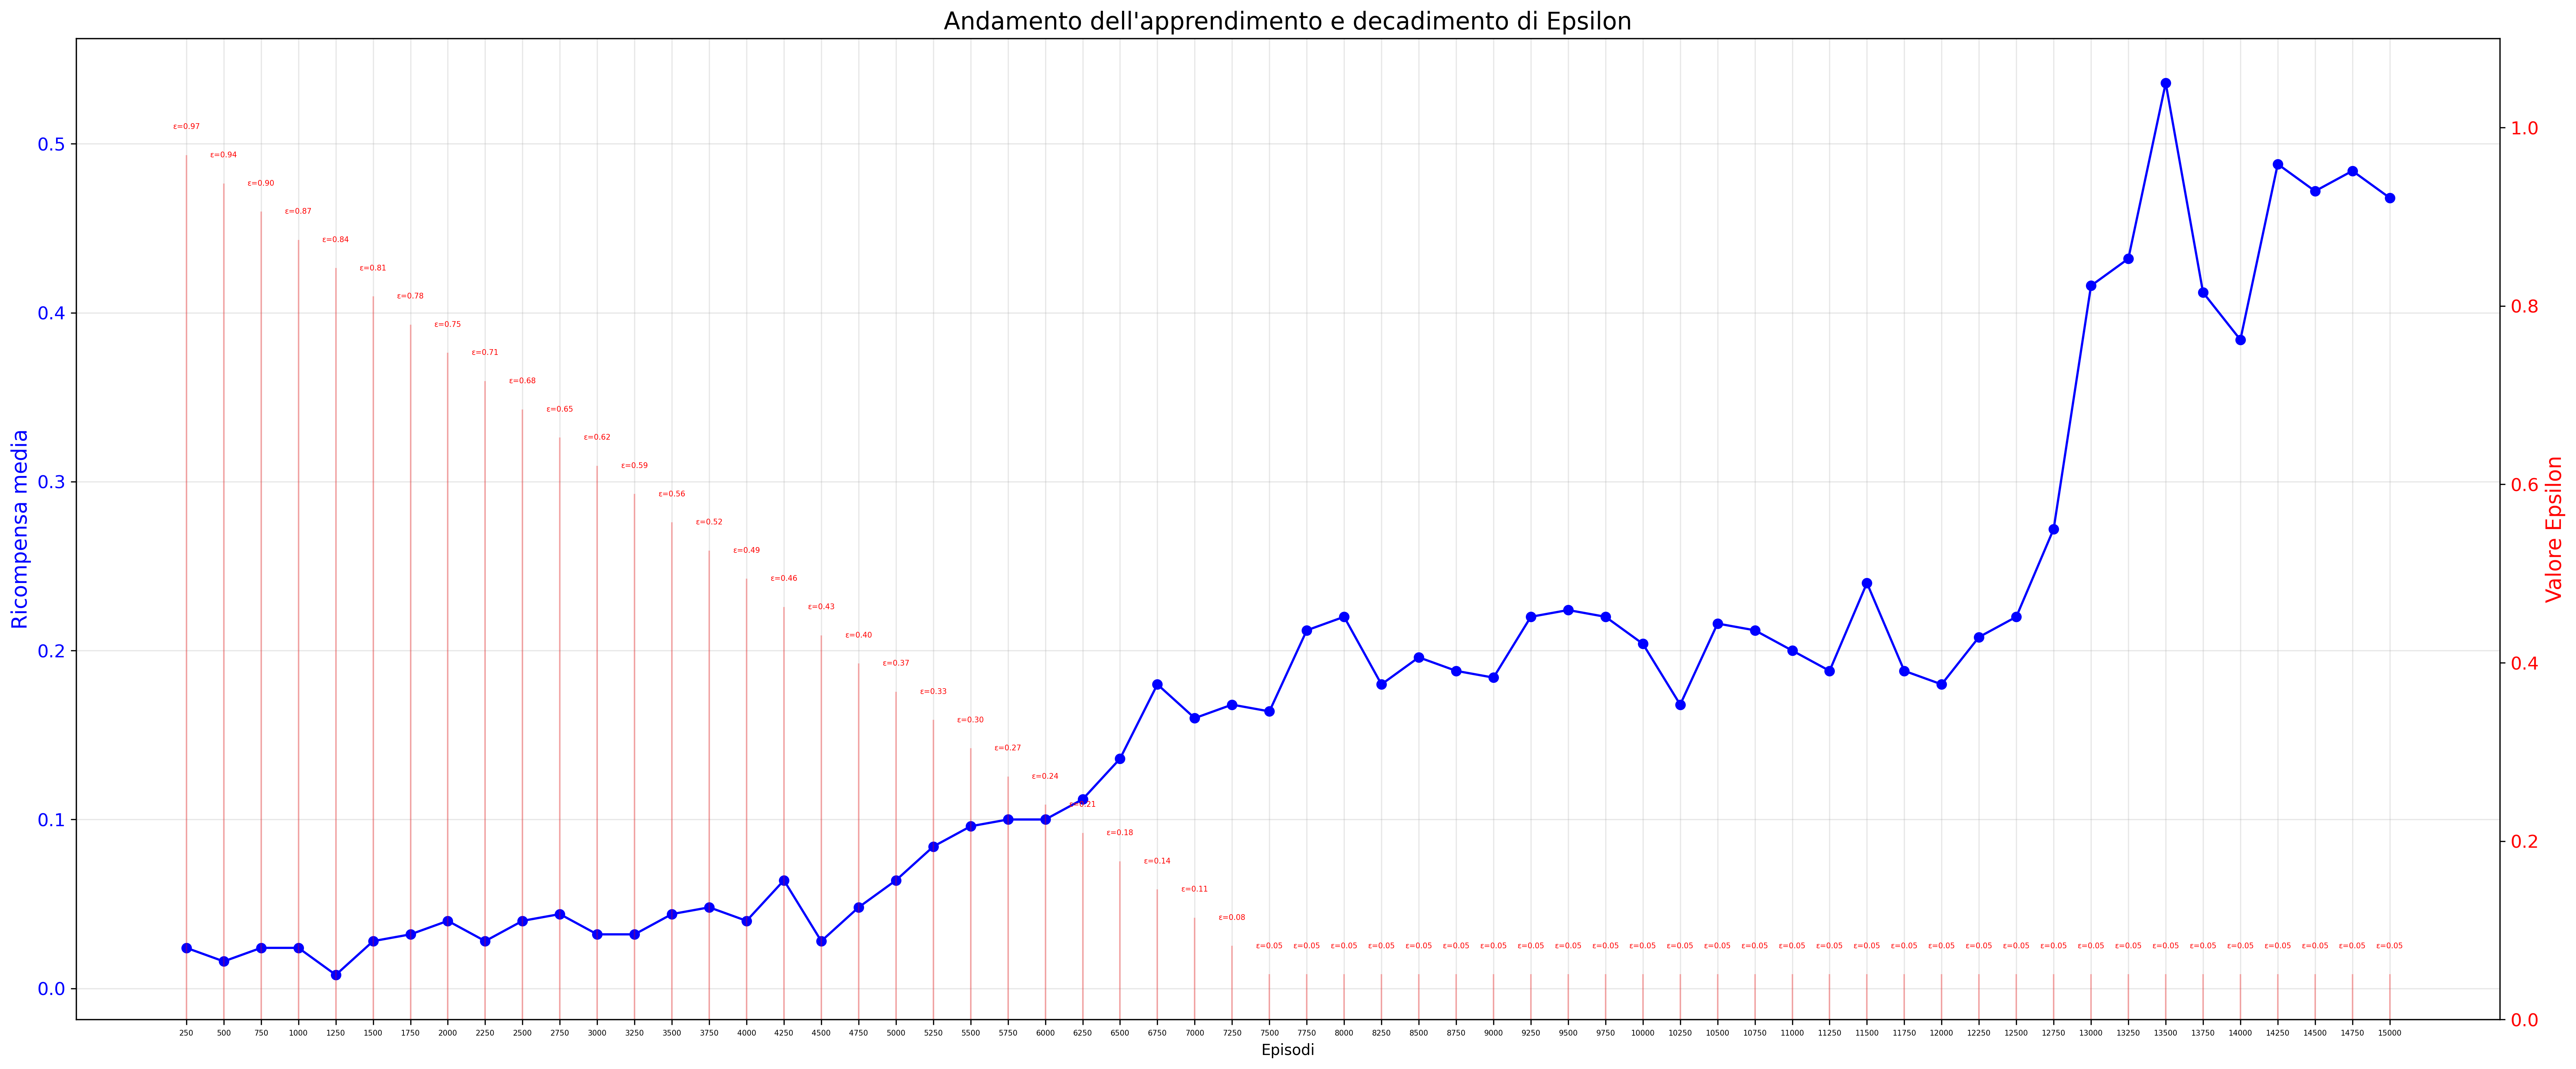
\includegraphics{TQL;lr=0.01;nep=15000;eps=1.0;fineps=0.05;eps_dec=0.00012666666666666666;gam=0.99.png}}
\end{center}

\begin{center}
\centering
\resizebox{\textwidth}{!}{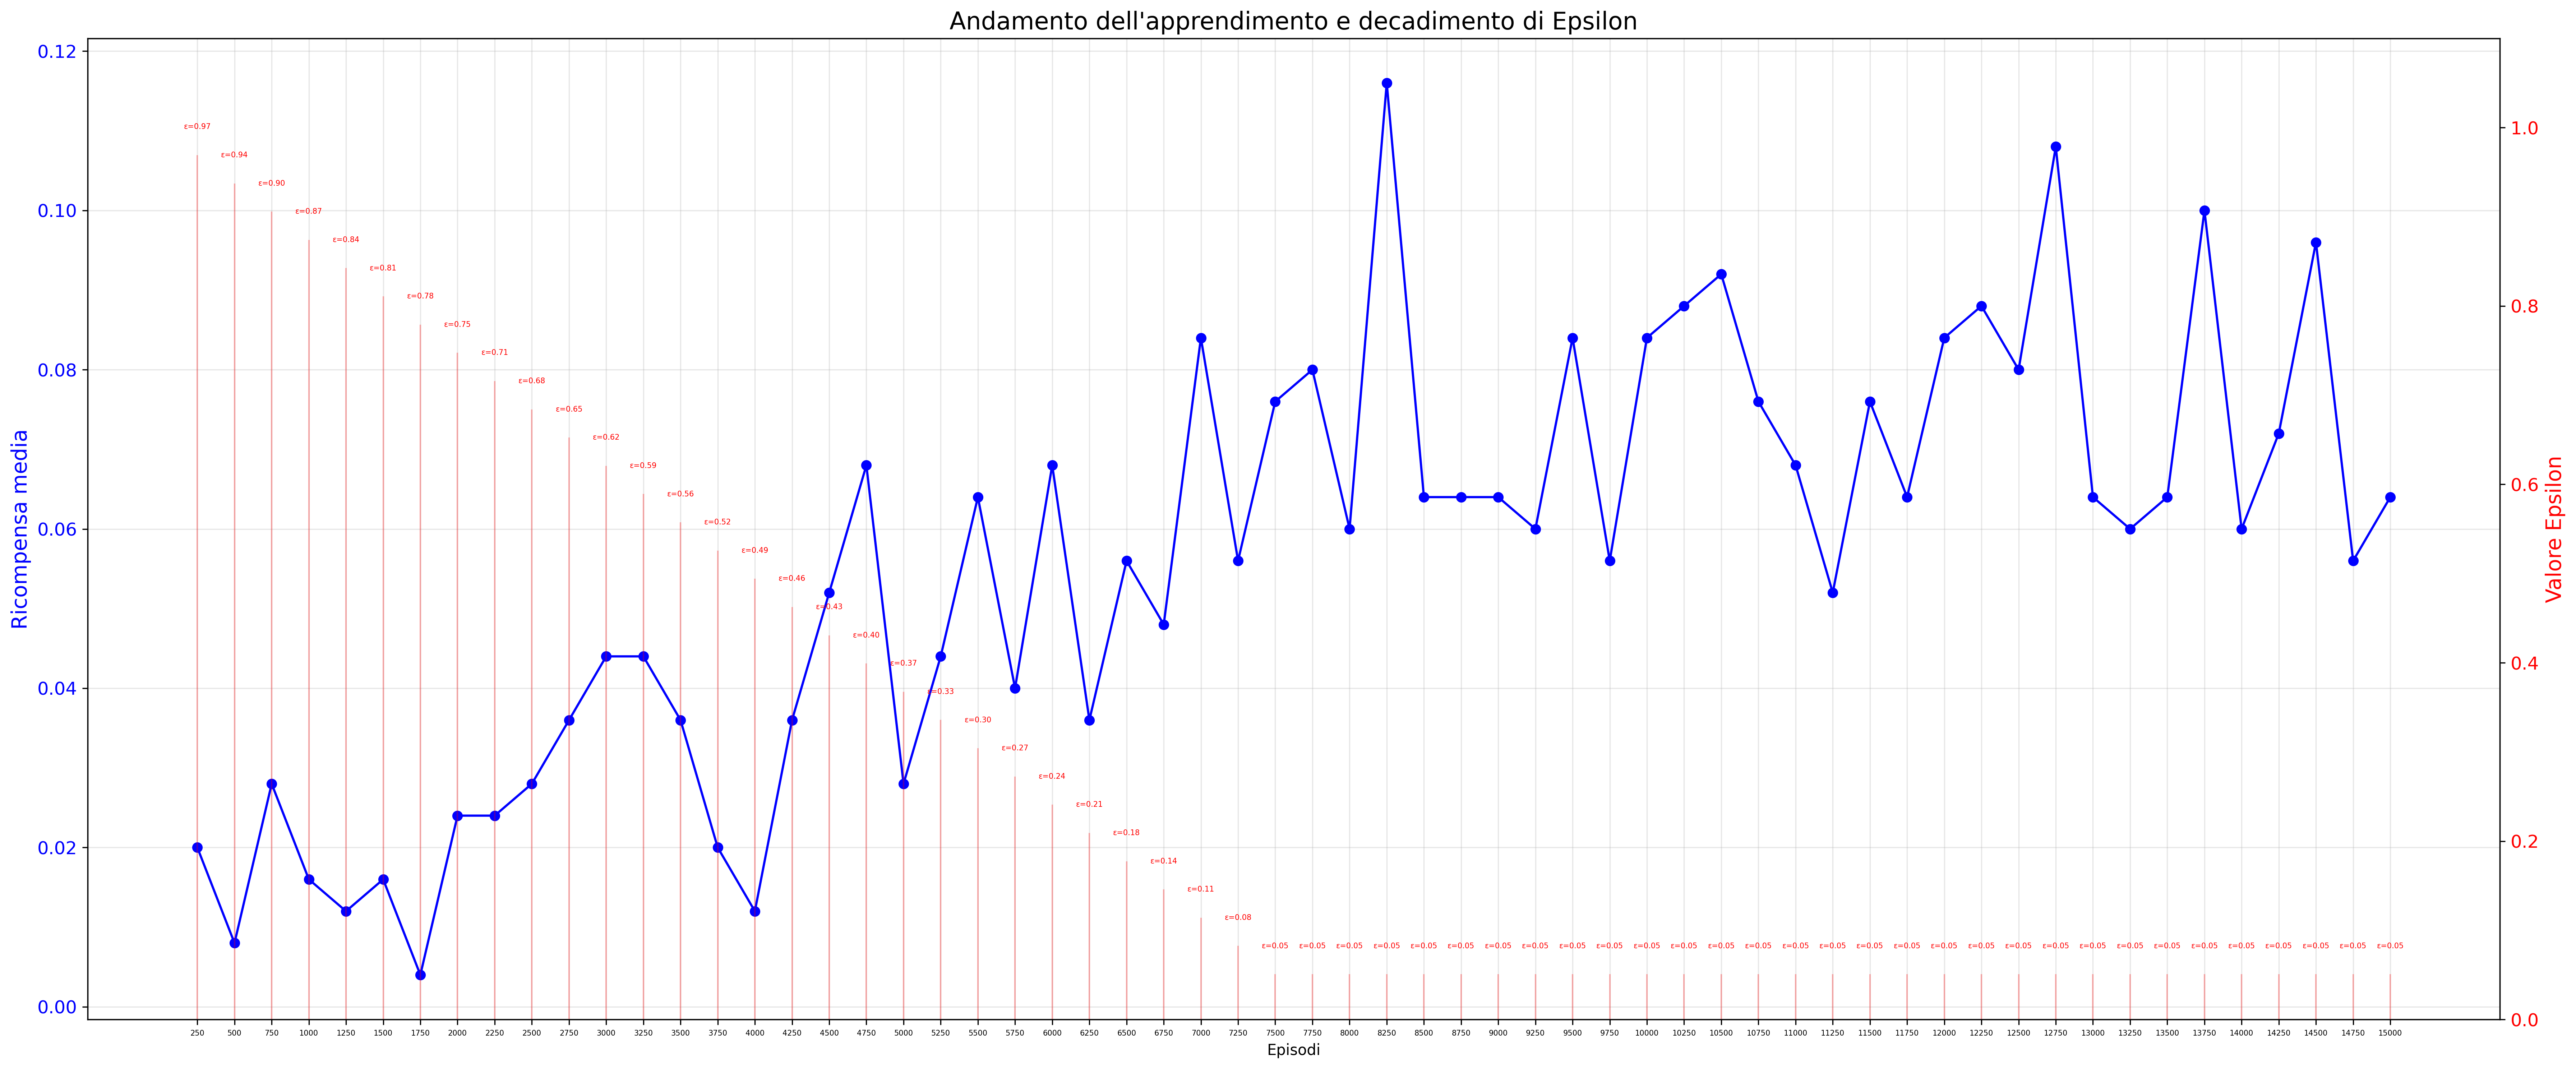
\includegraphics{TQL;lr=0.001;nep=15000;eps=1.0;fineps=0.05;eps_dec=0.00012666666666666666;gam=0.99.png}}
\end{center}

\clearpage


In terms of convergence time, the first solution (with a learning rate of 0.1) is the best, reaching convergence at around episode 7500.
\\
The second configuration reaches a convergence at episode 13000, while the third configuration converges at episode 8000.
\\
In terms of average cumulative reward at convergence, the first solution again performs the best, achieving a reward of 1 (reaching the goal) in 72.6\% of the episodes during the testing phase.
\\
The second solution has an average success rate of 59.6\%, while the third solution performs poorly, with an average success rate of only 6.2\% over the 500 testing episodes.

\subsubsection{Conclusions}

So, in conclusion, I would say that in the case of Tabular Q-learning in a non deterministic environment, the best configuration found is the following one:
\begin{itemize}
\item[--] $\alpha$= 0.1
\item[--] $\epsilon$ decay= 0.000126
\item[--] initial $\epsilon$ = 1
\item[--] final $\epsilon$ = 0.05
\item[--] gamma = 0.99
\end{itemize}


Bringing an average cumulative reward of 0.726 and converging in about 7500 episodes.

This is the policy obtained from the Q-table, which is the best one:
\begin{center}
    \centering
    \resizebox{\textwidth}{!}{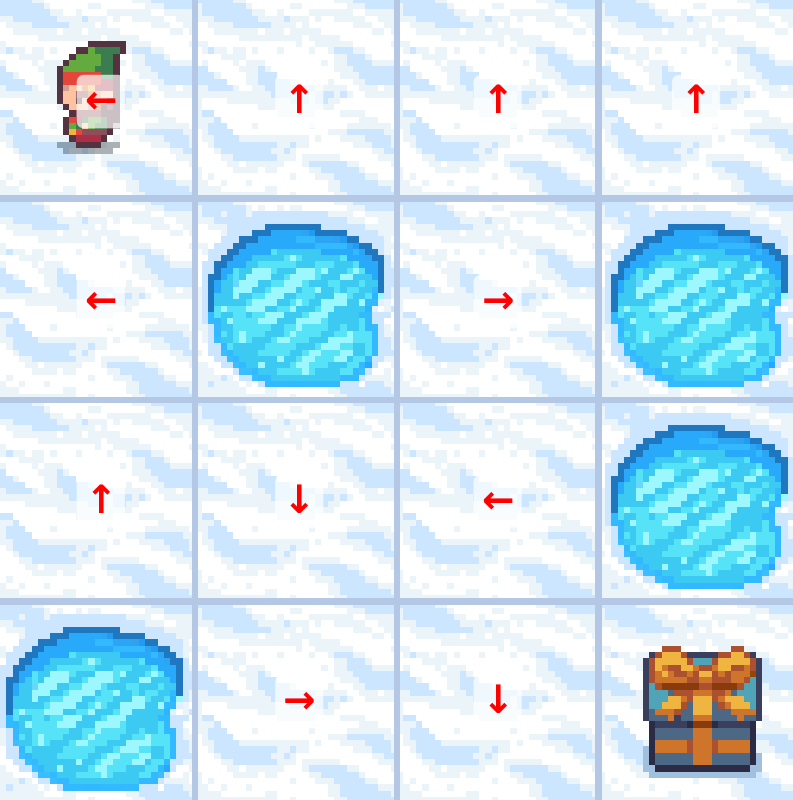
\includegraphics{policy_arrows_4x4.png}}
\end{center}
    

\section{Deep Q Network}

\subsection{Solution adopted}

\begin{center}
\centering
\resizebox{\textwidth}{!}{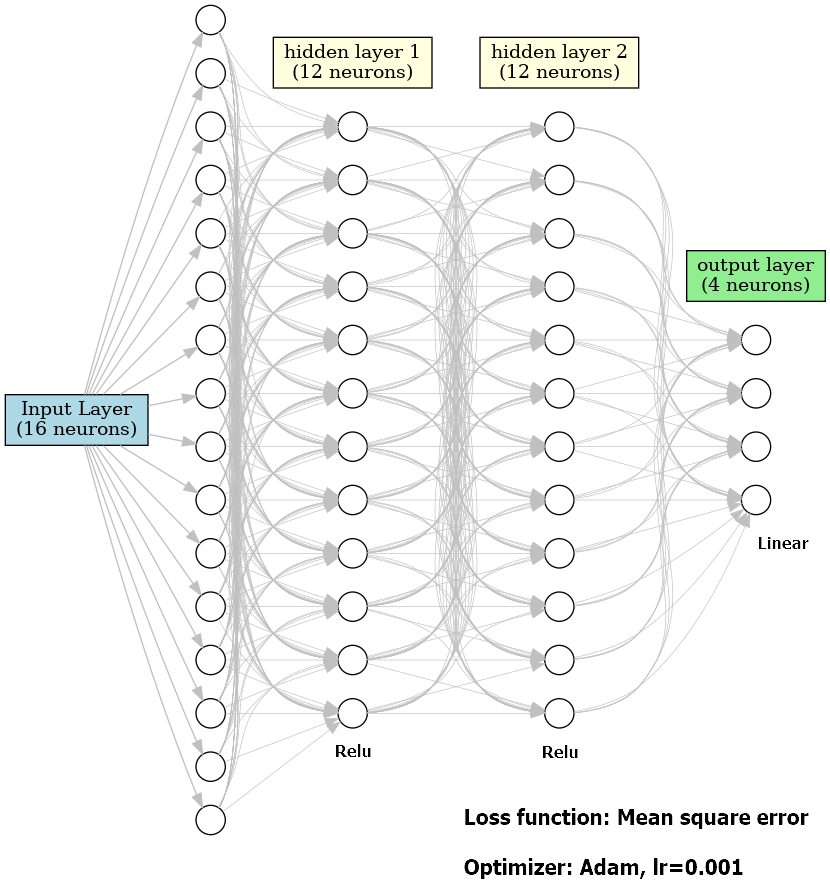
\includegraphics{NN_architecture.png}}
\end{center}

\clearpage

I have used tensorflow with keras for bulding a feedforward neural network for solving the Frozen Lake environment, using always the non deterministic Q learning technique.
\\
These are the characteristics of the network:
\begin{itemize}
\item[--] Feedforward neural network
\item[--] Width is 16, cause the number of neurons of the input layer
\item[--] Depth is 2, because we have 2 hidden layers
\item[--] The neurons are fully connected in a Dense way (each neuron is connected with all the following neurons)
\item[--] The activation function of the hidden layers is the Relu (Rectified linear units)
\item[--] The activation function of the output layer is the Linear (Identity function)
\item[--] The loss function used is the Mean Square Error
\item[--] The optimizer used is Adam, with a learning rate of 0.001
\item[--] The number of training episode is 15000
\item[--] The average cumulative reward is calculated over a range of 250 episodes
\item[--] The number of test episodes is 500
\item[--] The mini-batch size is 64
\end{itemize}

\begin{figure}[h]
    \centering
    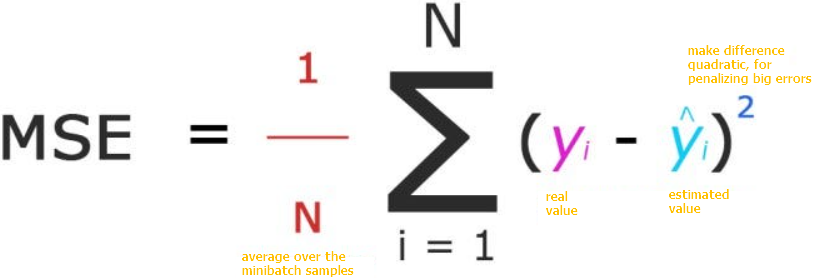
\includegraphics[width=0.8\textwidth]{Mean_square_error_function.png}
    \caption{Mean Square Error Loss function}
    \label{mse_loss:}

\end{figure}

The number of neurons in the neural network, and the type of connection (Dense), achieves the presence of 384 weight parameters.
\\
\\
\textbf{OPTIMIZER}
\\
The optimizers (which in this case is Adam), have the goal of adapting the learning rate value (starting from 0.001 in this case) with respect to the current iteration in the training phase; this is done because through the gradient of the loss function at each iteration, we have to perform an adjustment to the weights that contribute to the error.
\\
We want the adjustments to be bigger in the first iterations and lower in the later ones, and this is achieved by controlling how the learning rate influences the weight updates during the correction phase, which is the optimizers goal.
\\
\\
\textbf{LOSS FUNCTION}
\\
The loss function (which in this case is the mse), has the goal of calculate the difference between a predicted value and the actual value from the training dataset.
\\
\\
\textbf{ACTIVATION FUNCTION}
\\
The activation functions (Which in this case are the Relu: g($\alpha$) = max(0,$\alpha$) and the Linear: identity function) are the functions which applies to the weighted sum of the inputs to each neuron, giving the output.
\\
In the hidden layers they are not linear and aim to introduce non linearity, in order to be able to capture the non linear relationship between the states and their optimal Q values.
\\
To be precise, for computing the gradient on the loss function for correcting the weight's values, we are computing it also on the activation function, but we have no troubles cause the non derivability at the point x=0 (in the case of relu), because is almost impossible that we reach exactly that point during the training phase.
\\
\\
\textbf{REPLAY BUFFER}
\\
In reinforcement learning it is a data structure commonly used in algorithms like Q-learning.
\\
It stores tuples of the form (state, action, reward, next state) that are generated at each step during the training phase.
\\
When the neural network trains at each episode, it updates the model using only a sample (in this case, of size mini-batch = 64) from the total training data stored in the replay buffer. 
\\
This approach speeds up training by avoiding the need to train on the entire dataset at each iteration, which grows with each step.
\\
It is important to note that the values stored in the tuples are the ones needed and used to update the Q-values, which are then used for training.


\subsection{Metric results}


\subsubsection{Changing the epsilon decay}


These are the common hyper parameters for the runs:
\begin{itemize}
\item[--] $\alpha$= 0.1
\item[--] initial $\epsilon$ = 1
\item[--] final $\epsilon$ = 0.05
\item[--] gamma = 0.99
\end{itemize}

From the first plot to the third, the $\epsilon$ decay rate is increased as follows:

\begin{itemize}
\item[--] The first brings $\epsilon$ to its minimum value at 7/8 of the episodes.
\item[--] The second brings $\epsilon$ to the minimum at 3/4 of the episodes.
\item[--] The last one brings $\epsilon$ to the minimum at 1/2 of the total episodes.
\end{itemize}


\begin{center}
\centering
\resizebox{\textwidth}{!}{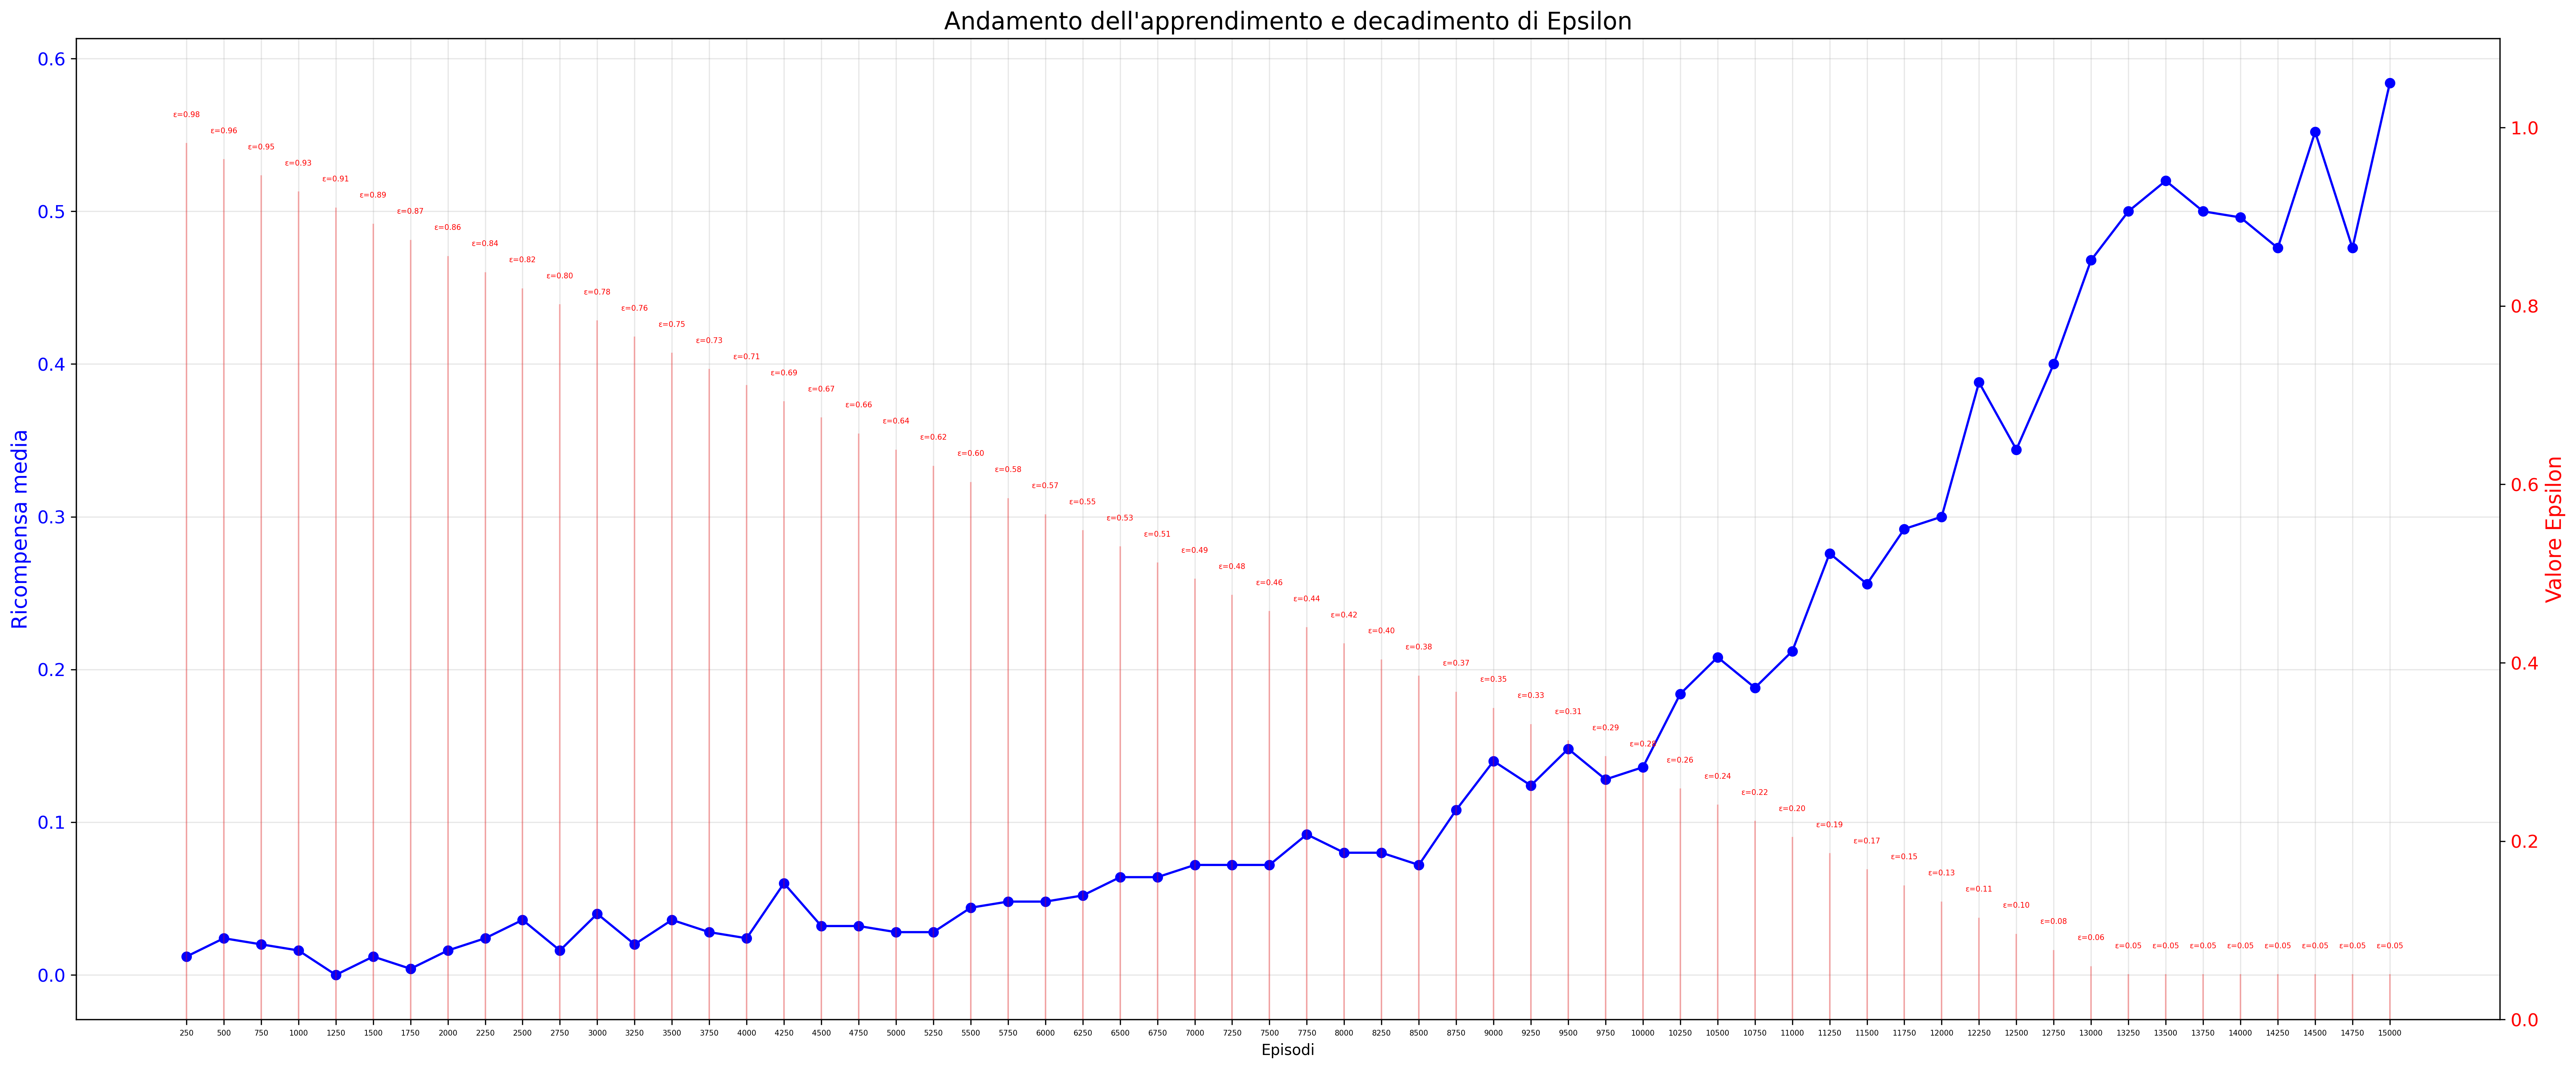
\includegraphics{DQN;lr=0.1;nep=15000;eps=1.0;fineps=0.05;eps_dec=7.238095238095238e-05;gam=0.99.png}}
\end{center}

\begin{center}
\centering
\resizebox{\textwidth}{!}{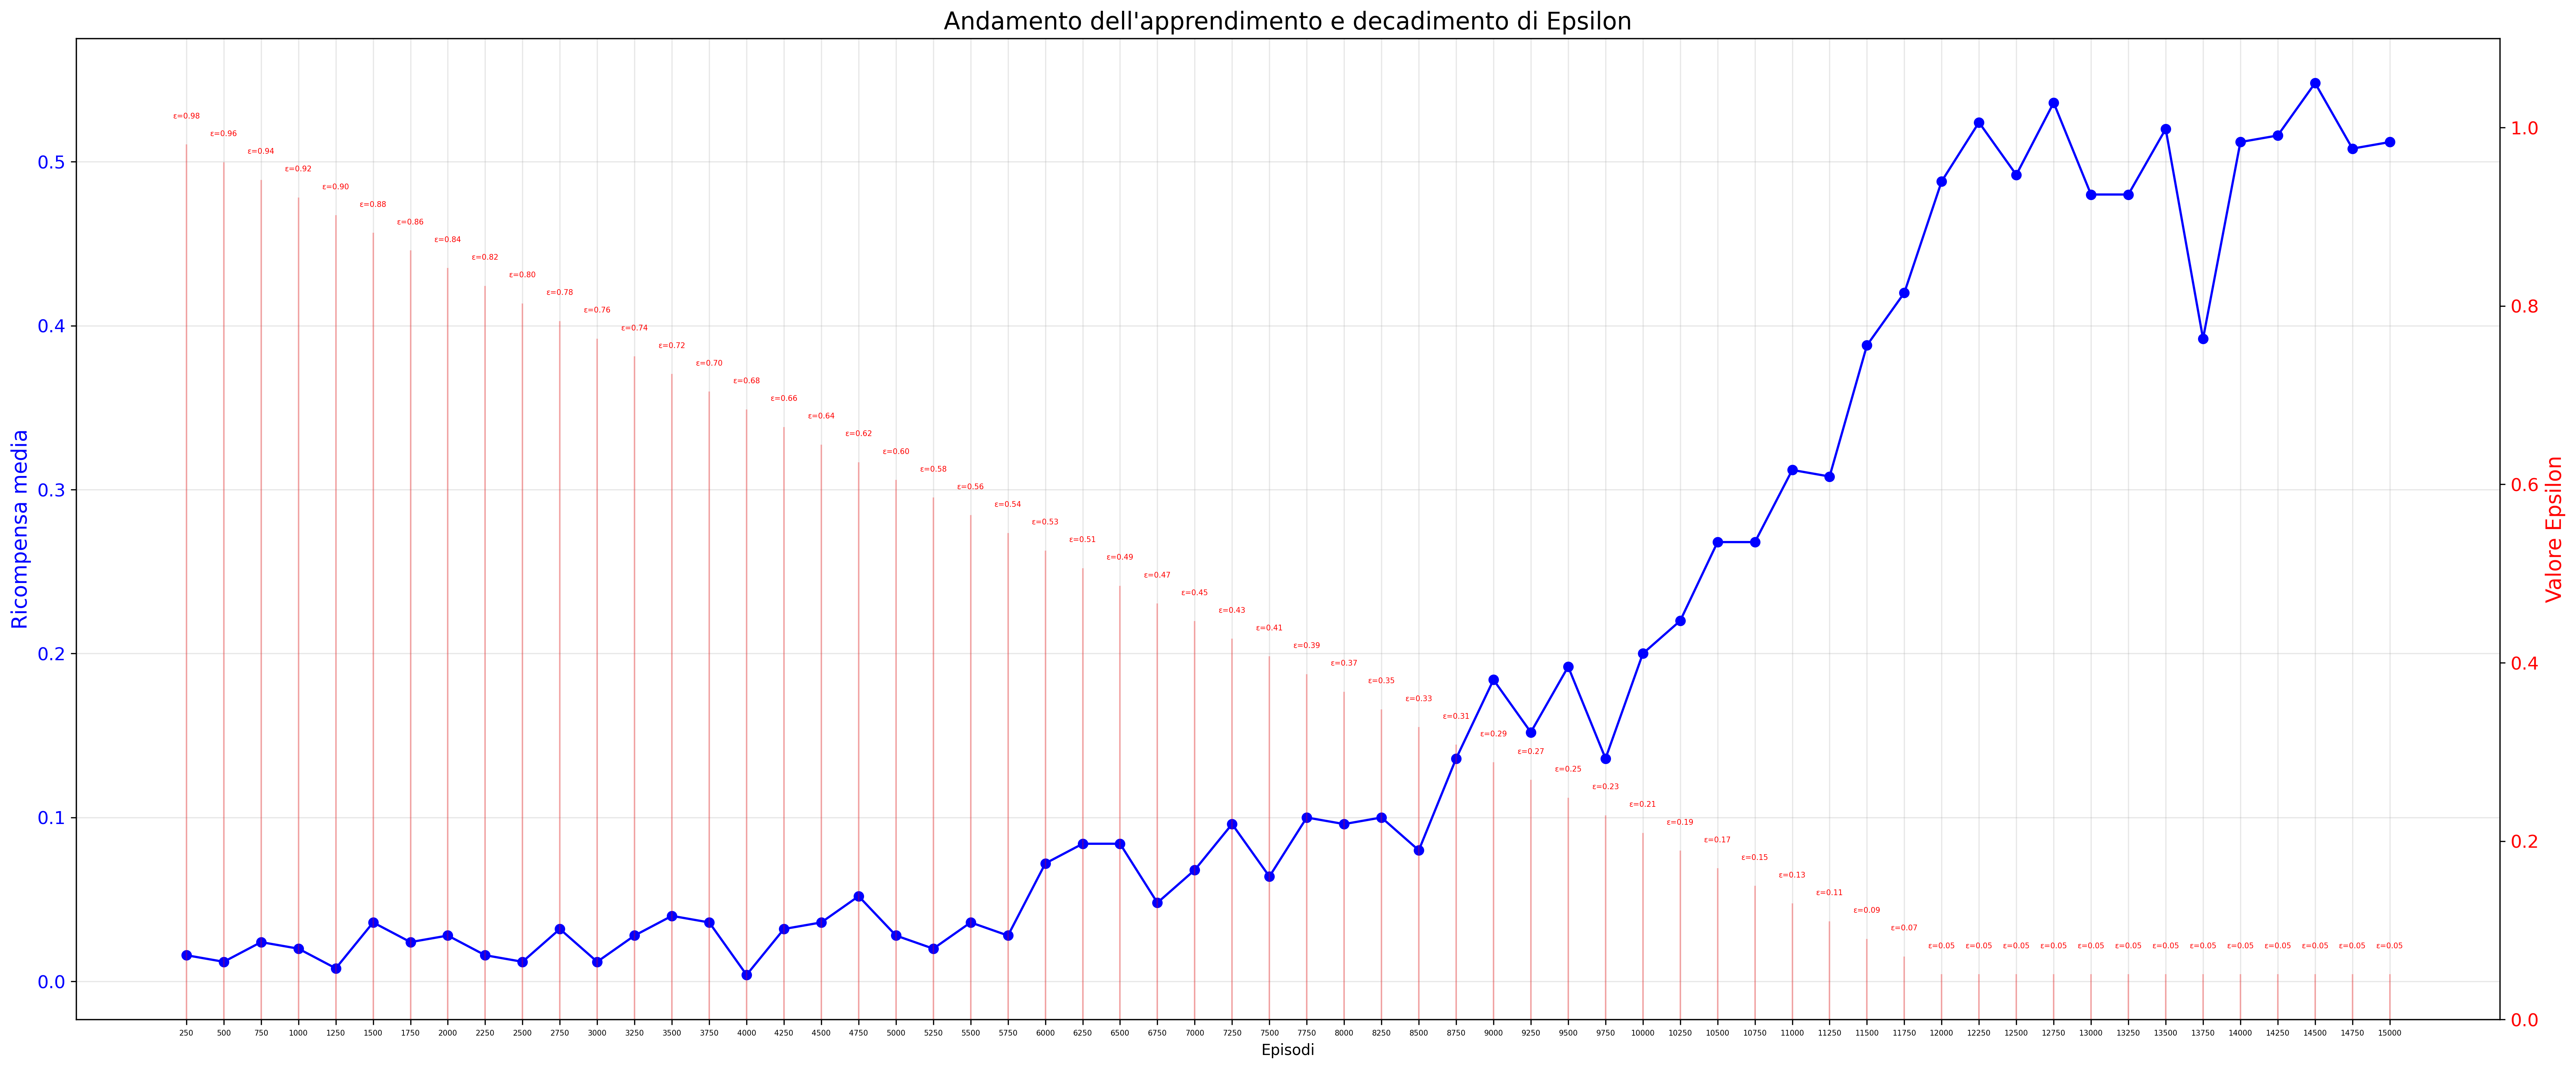
\includegraphics{DQN;lr=0.1;nep=15000;eps=1.0;fineps=0.05;eps_dec=7.916666666666666e-05;gam=0.99.png}}
\end{center}

\begin{center}
\centering
\resizebox{\textwidth}{!}{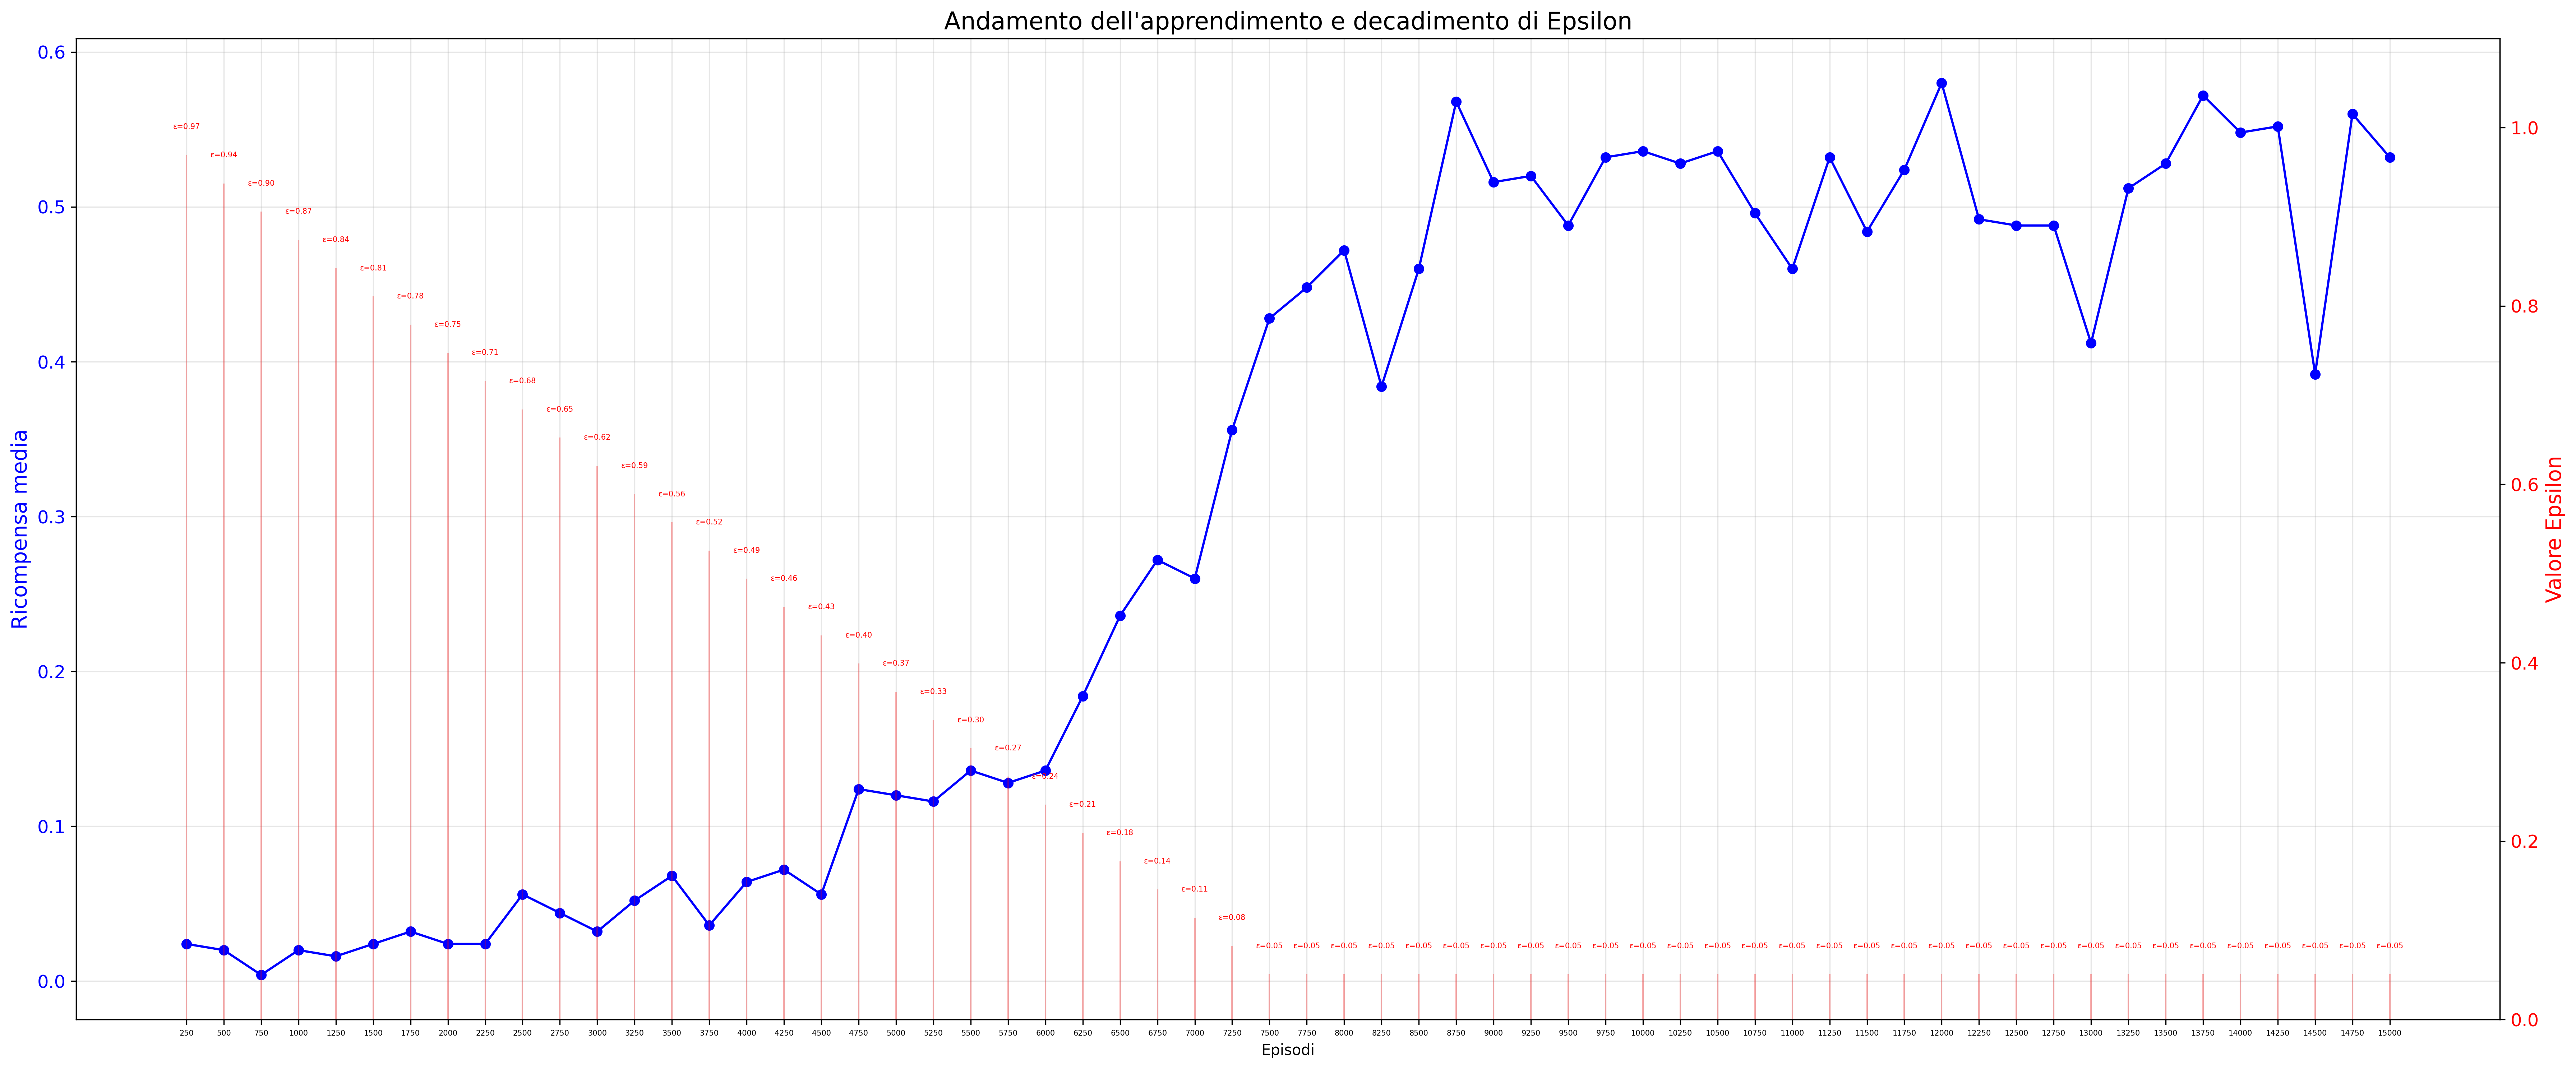
\includegraphics{DQN;lr=0.1;nep=15000;eps=1.0;fineps=0.05;eps_dec=0.00012666666666666666;gam=0.99.png}}
\end{center}

\clearpage


In the first configuration (with $\epsilon$ which goes to the minimum at 7/8 of the episodes) the convergence is achieved almost at the 13250 episode.
\\
In the second, instead, the convergence is achieved at 12250 episodes, then the third configuration is the best, converging on the 9000 episode.
\\
If we focus on the average cumulative reward at convergence, we could say that the first configuration is slightly better, achieving a success rate of the 52\%, against a 50\% achieved by the other two configurations.
\\
Now, considering the testing phase, which is done on 500 epsiodes: the second and third configurations are the best, having a 73.4\% of success rate, then the first achieves the 72.6\%.
\\
So, we can conclude that in terms of cumulative rewards, all the three possibilities has slightly the same performances, so I would say that the third configuration is the best, due to its faster convergence time.


\subsubsection{Changing the learning rate}


These are the common hyper parameters for the runs:
\begin{itemize}
\item[--] $\epsilon$ decay= 0.000126
\item[--] initial $\epsilon$ = 1
\item[--] final $\epsilon$ = 0.05
\item[--] gamma = 0.99
\end{itemize}

From the first plot to the third, the $\alpha$ value assumes the following values :
\begin{itemize}
\item[--] The first sets $\alpha$ to 0.1
\item[--] The second sets $\alpha$ to 0.01
\item[--] The third sets $\alpha$ to 0.001
\end{itemize}

\clearpage


\begin{center}
\centering
\resizebox{\textwidth}{!}{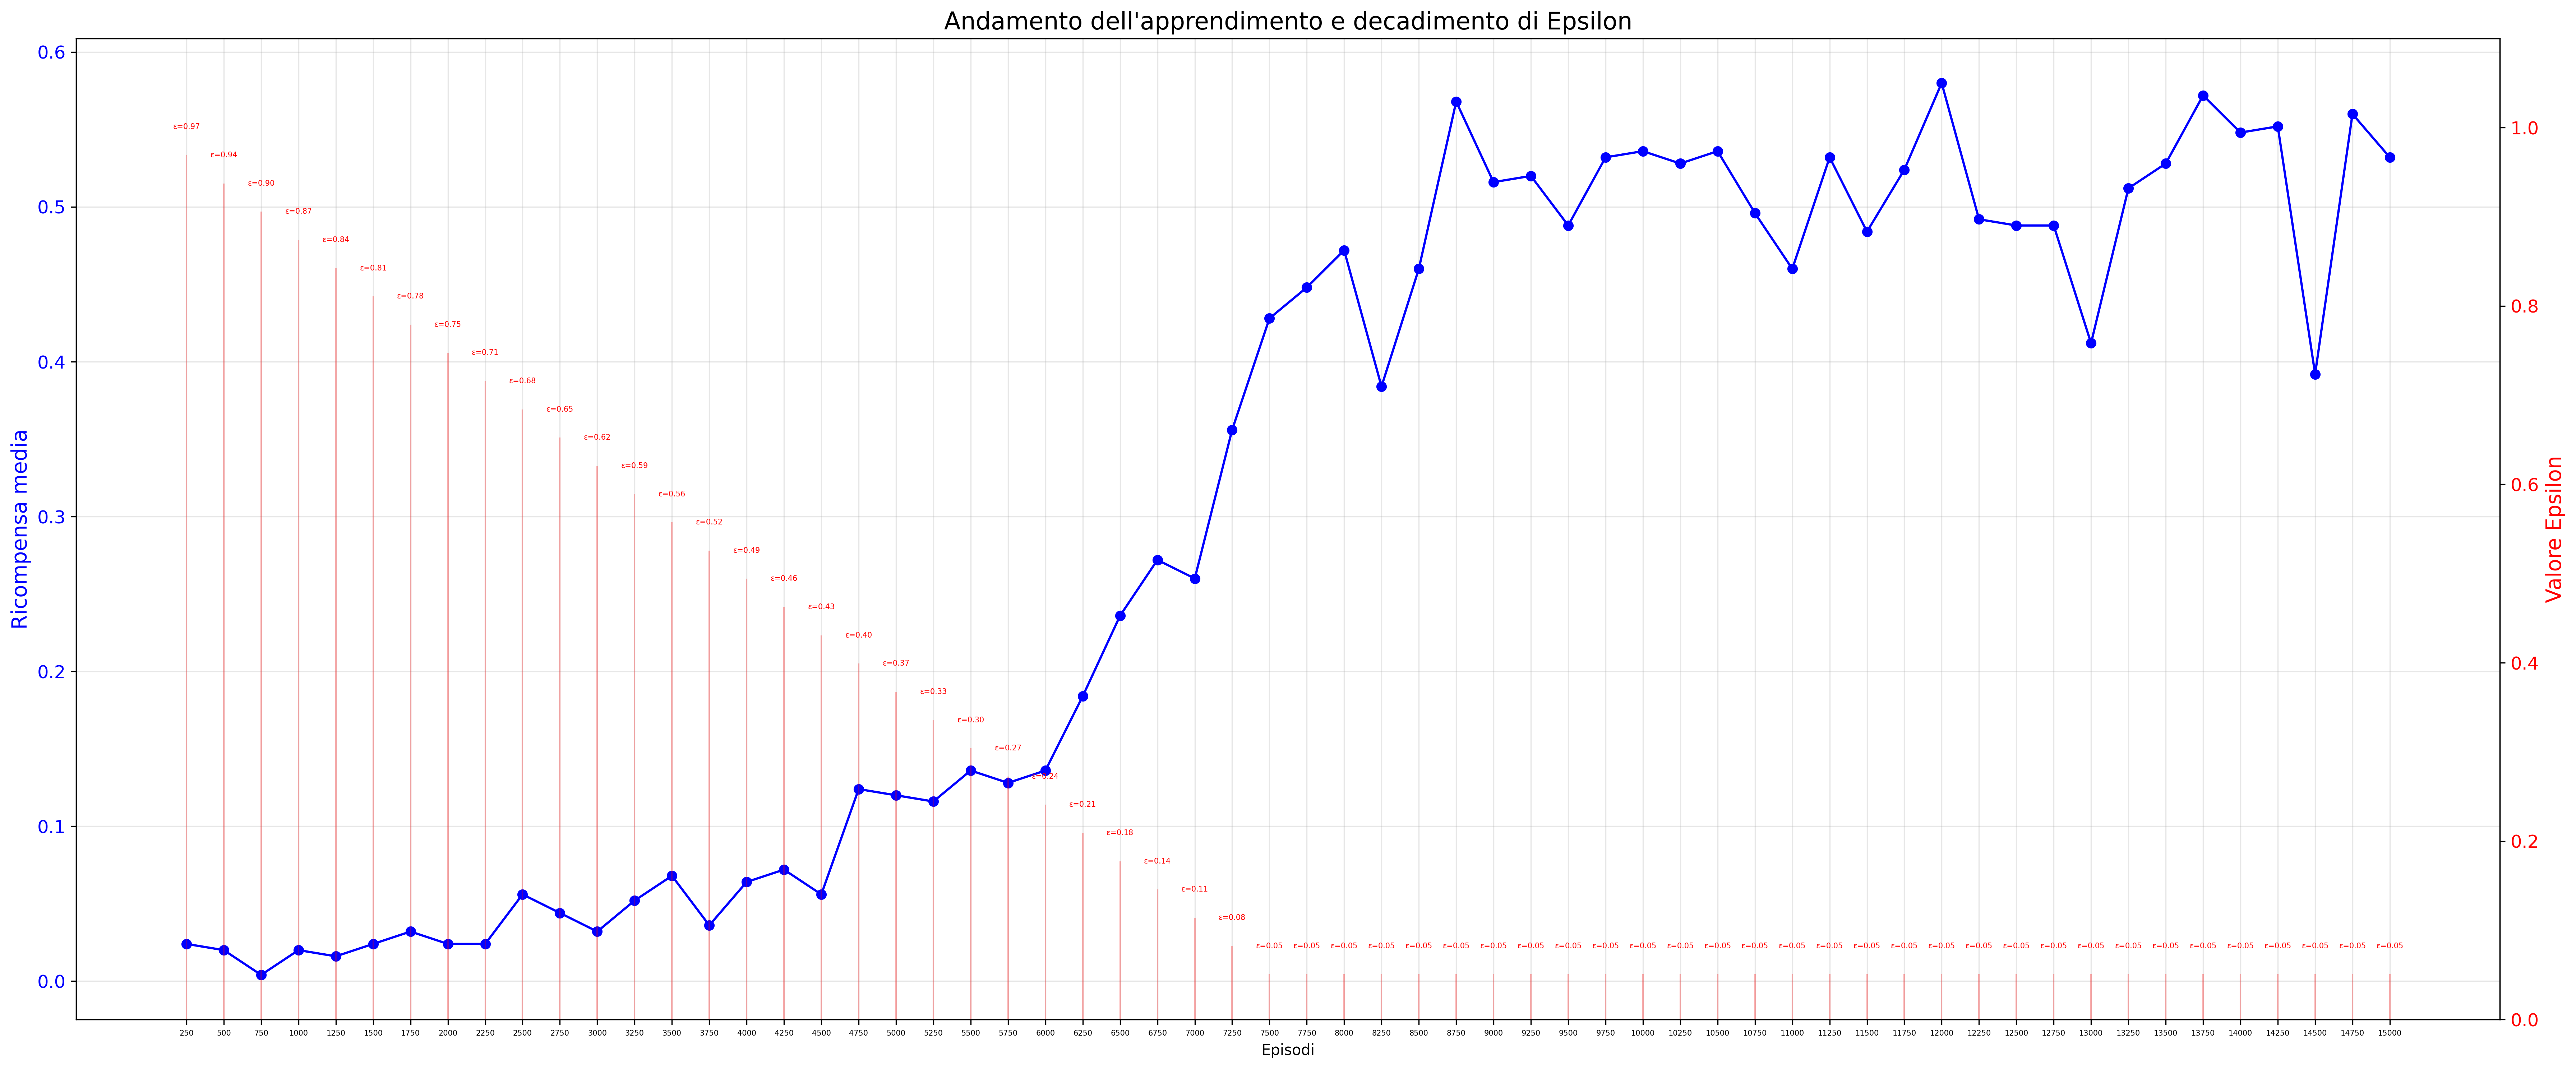
\includegraphics{DQN;lr=0.1;nep=15000;eps=1.0;fineps=0.05;eps_dec=0.00012666666666666666;gam=0.99.png}}
\end{center}

\begin{center}
\centering
\resizebox{\textwidth}{!}{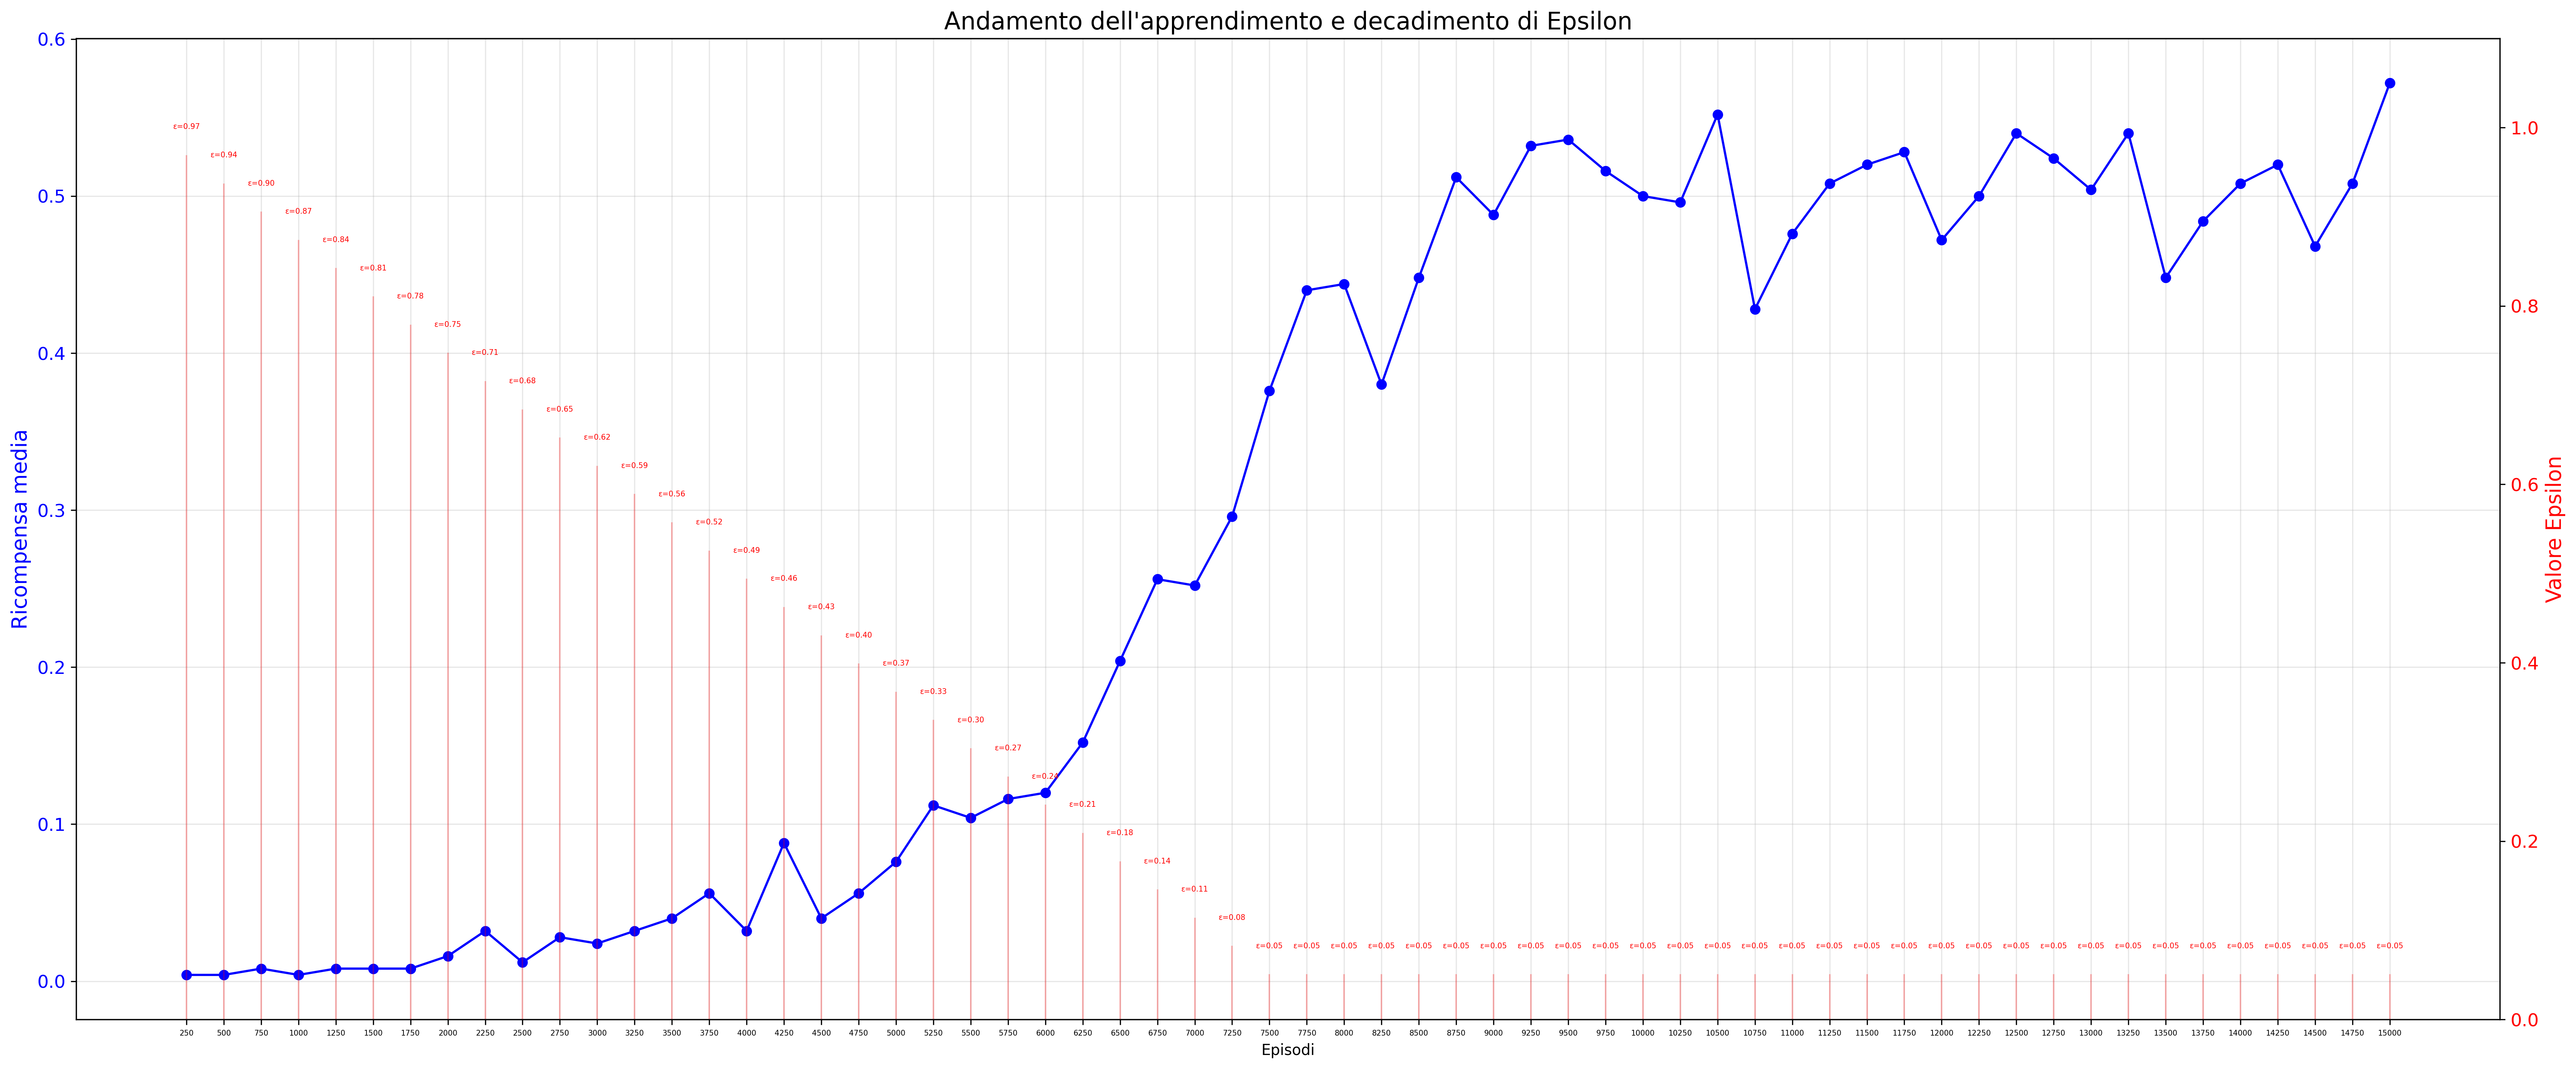
\includegraphics{DQN;lr=0.01;nep=15000;eps=1.0;fineps=0.05;eps_dec=0.00012666666666666666;gam=0.99.png}}
\end{center}

\begin{center}
\centering
\resizebox{\textwidth}{!}{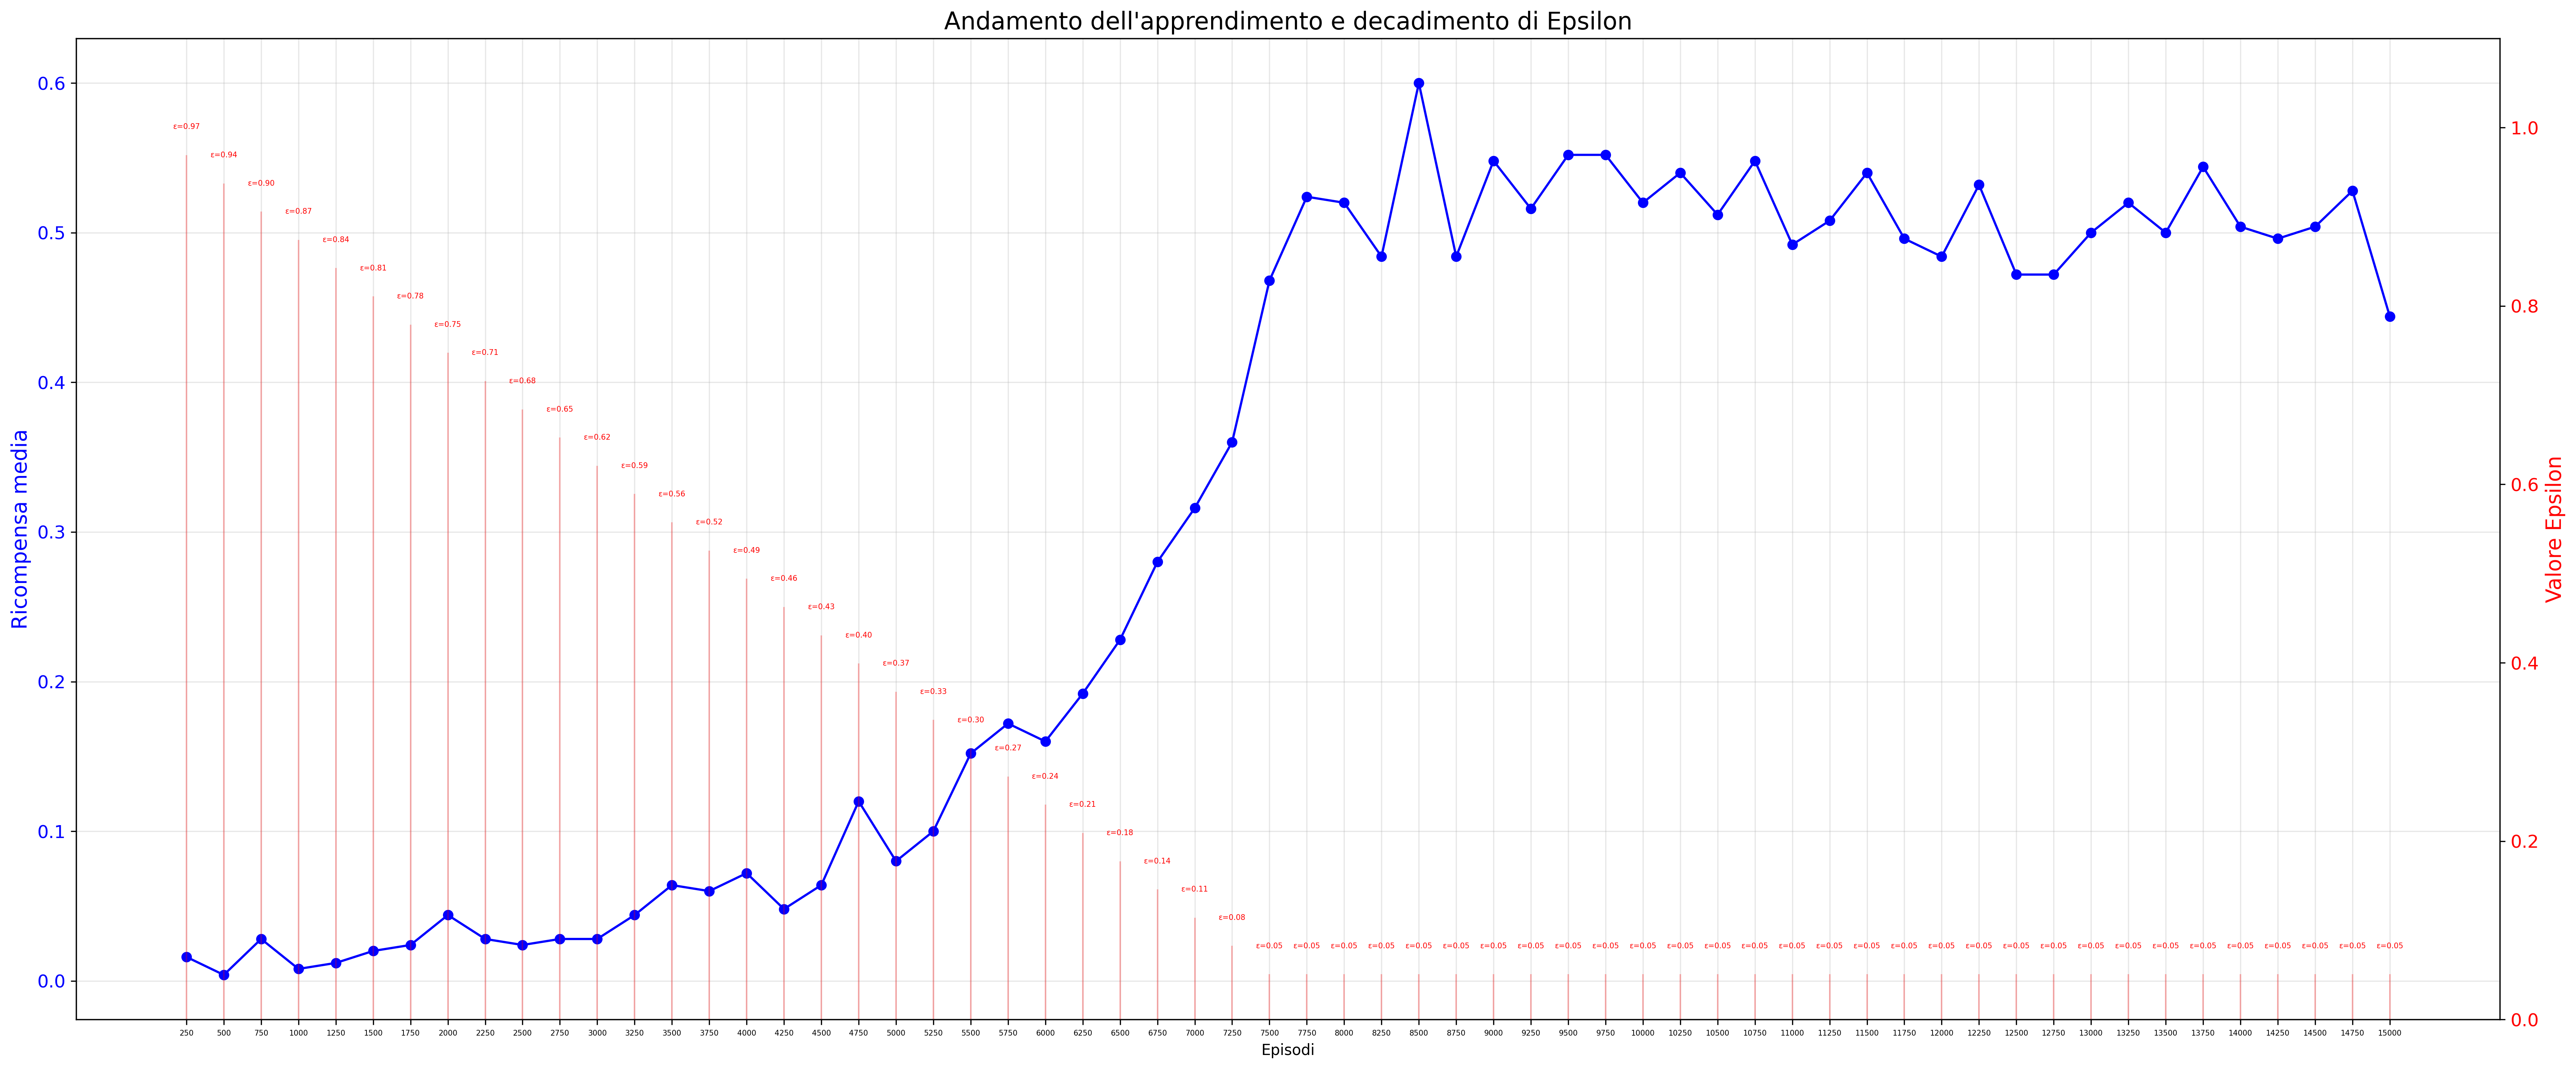
\includegraphics{DQN;lr=0.001;nep=15000;eps=1.0;fineps=0.05;eps_dec=0.00012666666666666666;gam=0.99.png}}
\end{center}

\clearpage


Considering the convergence time, the third configuration is the best, achieving that after 7750 episodes, but also the other ones don't behave badly, given that the first configuration converge after 
9000 epsiodes and the second one after 8750.
\\
With respect to the average cumulative reward at convergence aspect, both the first and the second one brings a success rate of 50\%, then the third one of 53\%.
\\
In terms of reward obtained in the testing phase, the second configuration is the best, bringing an average success rate of 75.2\%, instead, the first one brings the 73.4\% and the third,
which is slightly the worst one, bring success rate of the 72\%.
\\
In conclusion, I would say that both the three possibilities are similar in terms of performance, with the second one that takes some more episodes wrt the third one, but brings the best reward on the testing phase.


\subsubsection{Conclusions}

So, in conclusion, I would say that in the case of Deep Q Network in a non deterministic environment, the best configuration found is the following one:
\begin{itemize}
\item[--] $\alpha$= 0.01
\item[--] $\epsilon$ decay= 0.000126
\item[--] initial $\epsilon$ = 1
\item[--] final $\epsilon$ = 0.05
\item[--] gamma = 0.99
\end{itemize}

Bringing an average cumulative reward of 0.752 and converging in about 8750 episodes.   




\section{Map 8x8}

I have noticed that using a map with only 16 states, both DQN and TQL have the ability of approximating in an accurate way the Q table (using the best settings), obtaining a success rate of 70\%, which is the best achievable result in this stochastic environment.
So, for observing the performance differences between the two approaches, I have decided to perform the analysis on a bigger map (8x8), so having 64 possible states, with the same previous characteristics.

The following results come out from the same previous algorithms, following also the same settings of the hyper parameters, with some small changes.

\section{Tabular Q Learning}

\subsection{Solution adopted}

The agent algorithm has those changed characteristics:
\begin{itemize}
\item[--] In the training phase, now we have a range of 200 episodes for calculating the average cumulative reward over that range of episodes, so limiting the noise, but having more values on the plots
\item[--] In the test phase, a number of 2000 episodes, for having a more accurate value in output
\end{itemize}

\subsection{Metric results}

\subsubsection{Changing the epsilon decay}

As already said, the hyper parameters for the runs are the same as previous.
\\
From the first plot to the third, the $\epsilon$ decay rate is increased as follows (as previously described):
\begin{itemize}
\item[--] The first brings $\epsilon$ to its minimum value at 7/8 of the episodes.
\item[--] The second brings $\epsilon$ to the minimum at 3/4 of the episodes.
\item[--] The last one brings $\epsilon$ to the minimum at 1/2 of the total episodes.
\end{itemize}

\begin{center}
\centering
\resizebox{\textwidth}{!}{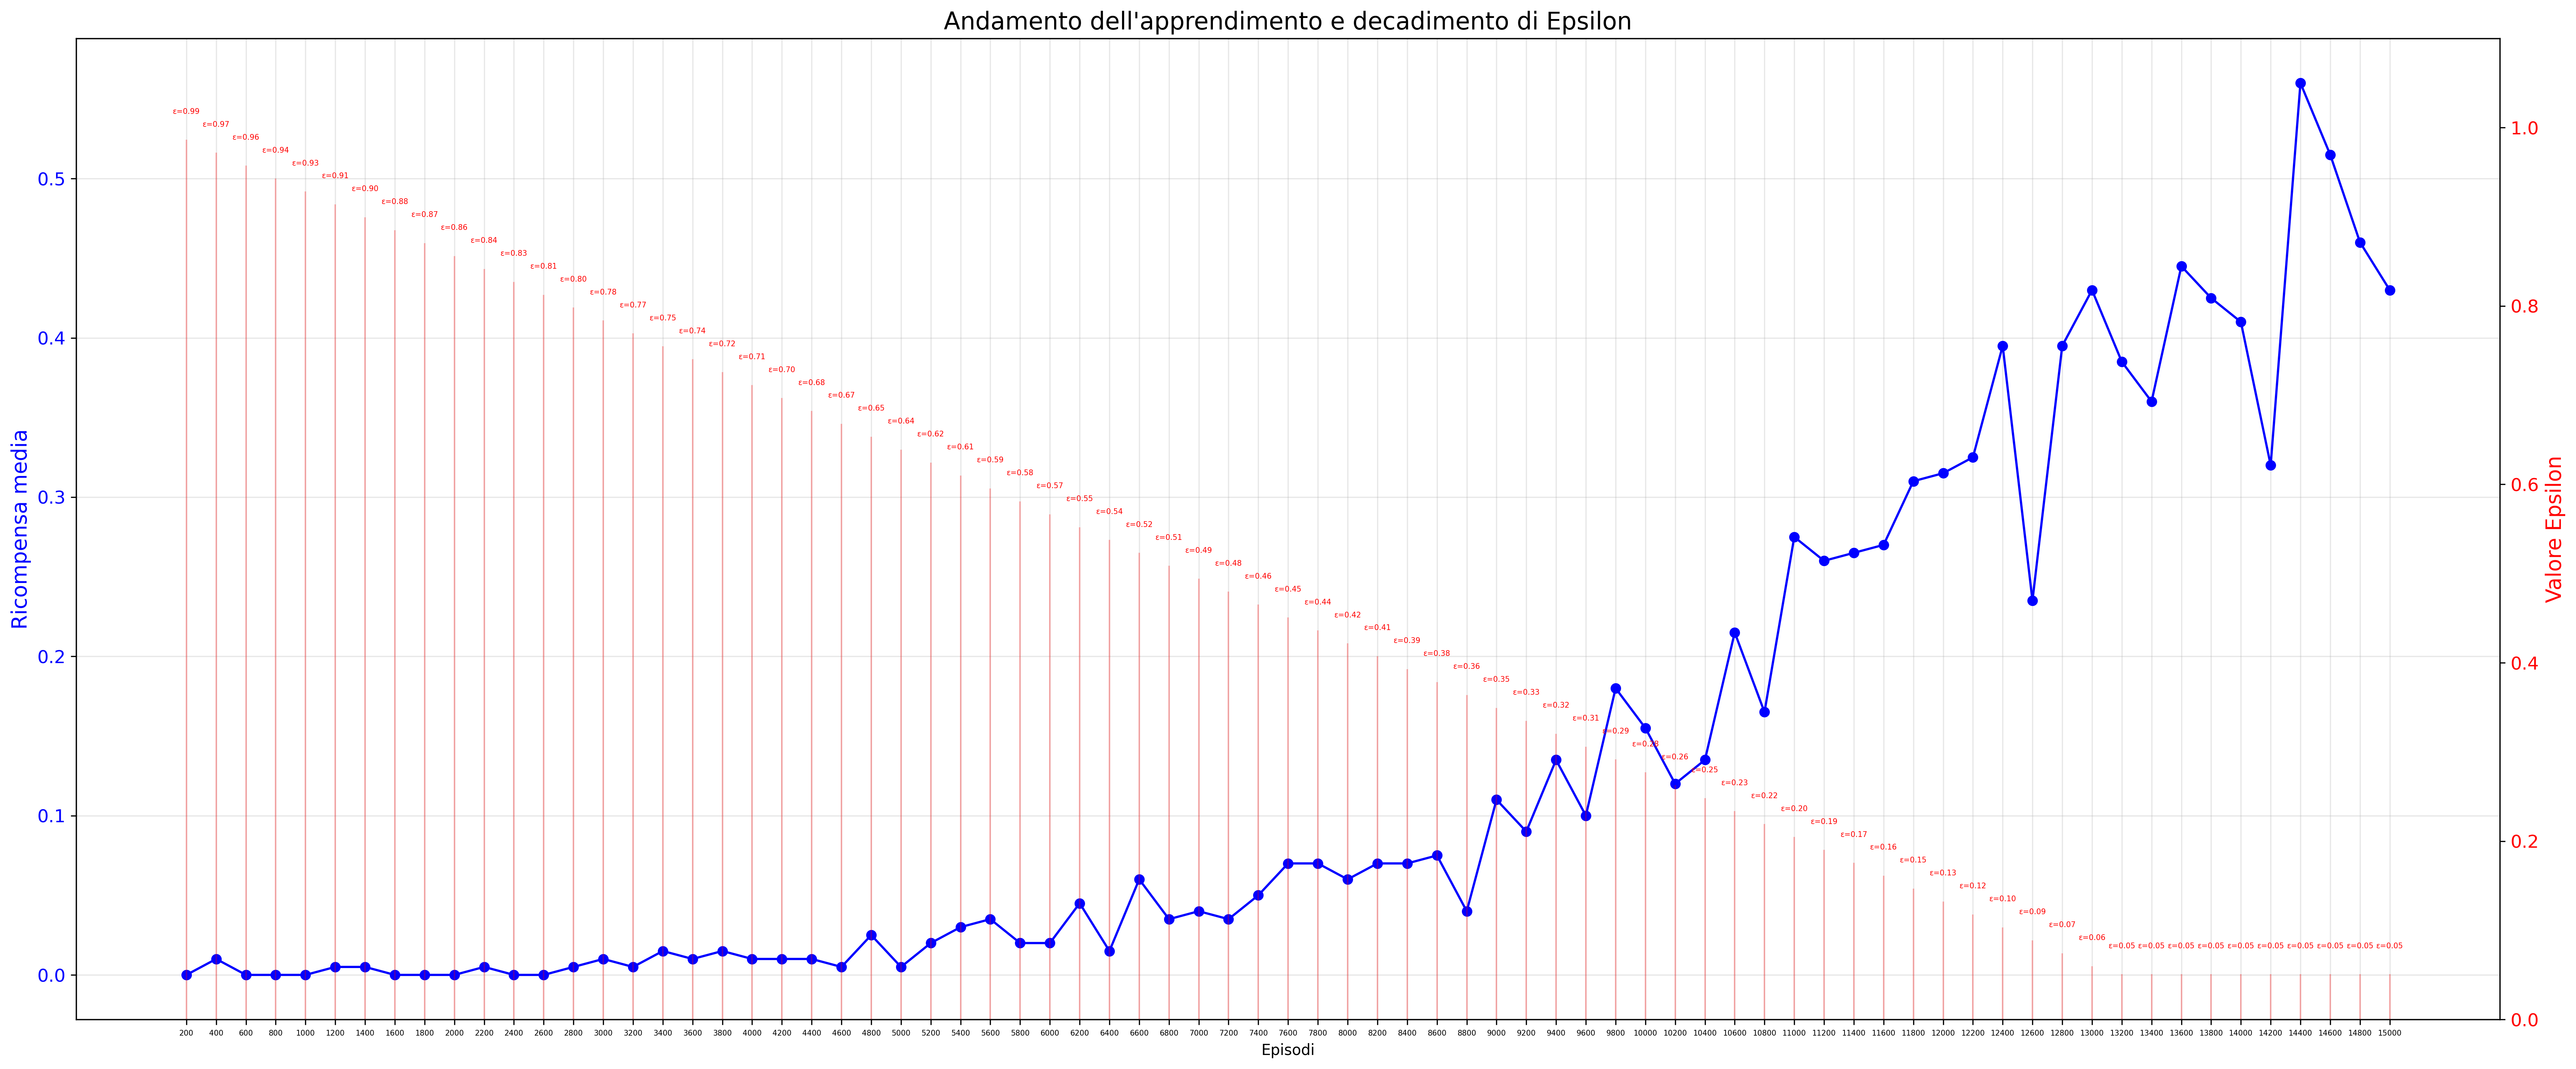
\includegraphics{TQL2;lr=0.1;nep=15000;eps=1.0;fineps=0.05;eps_dec=7.238095238095238e-05;gam=0.99.png}}
\end{center}


\begin{center}
\centering
\resizebox{\textwidth}{!}{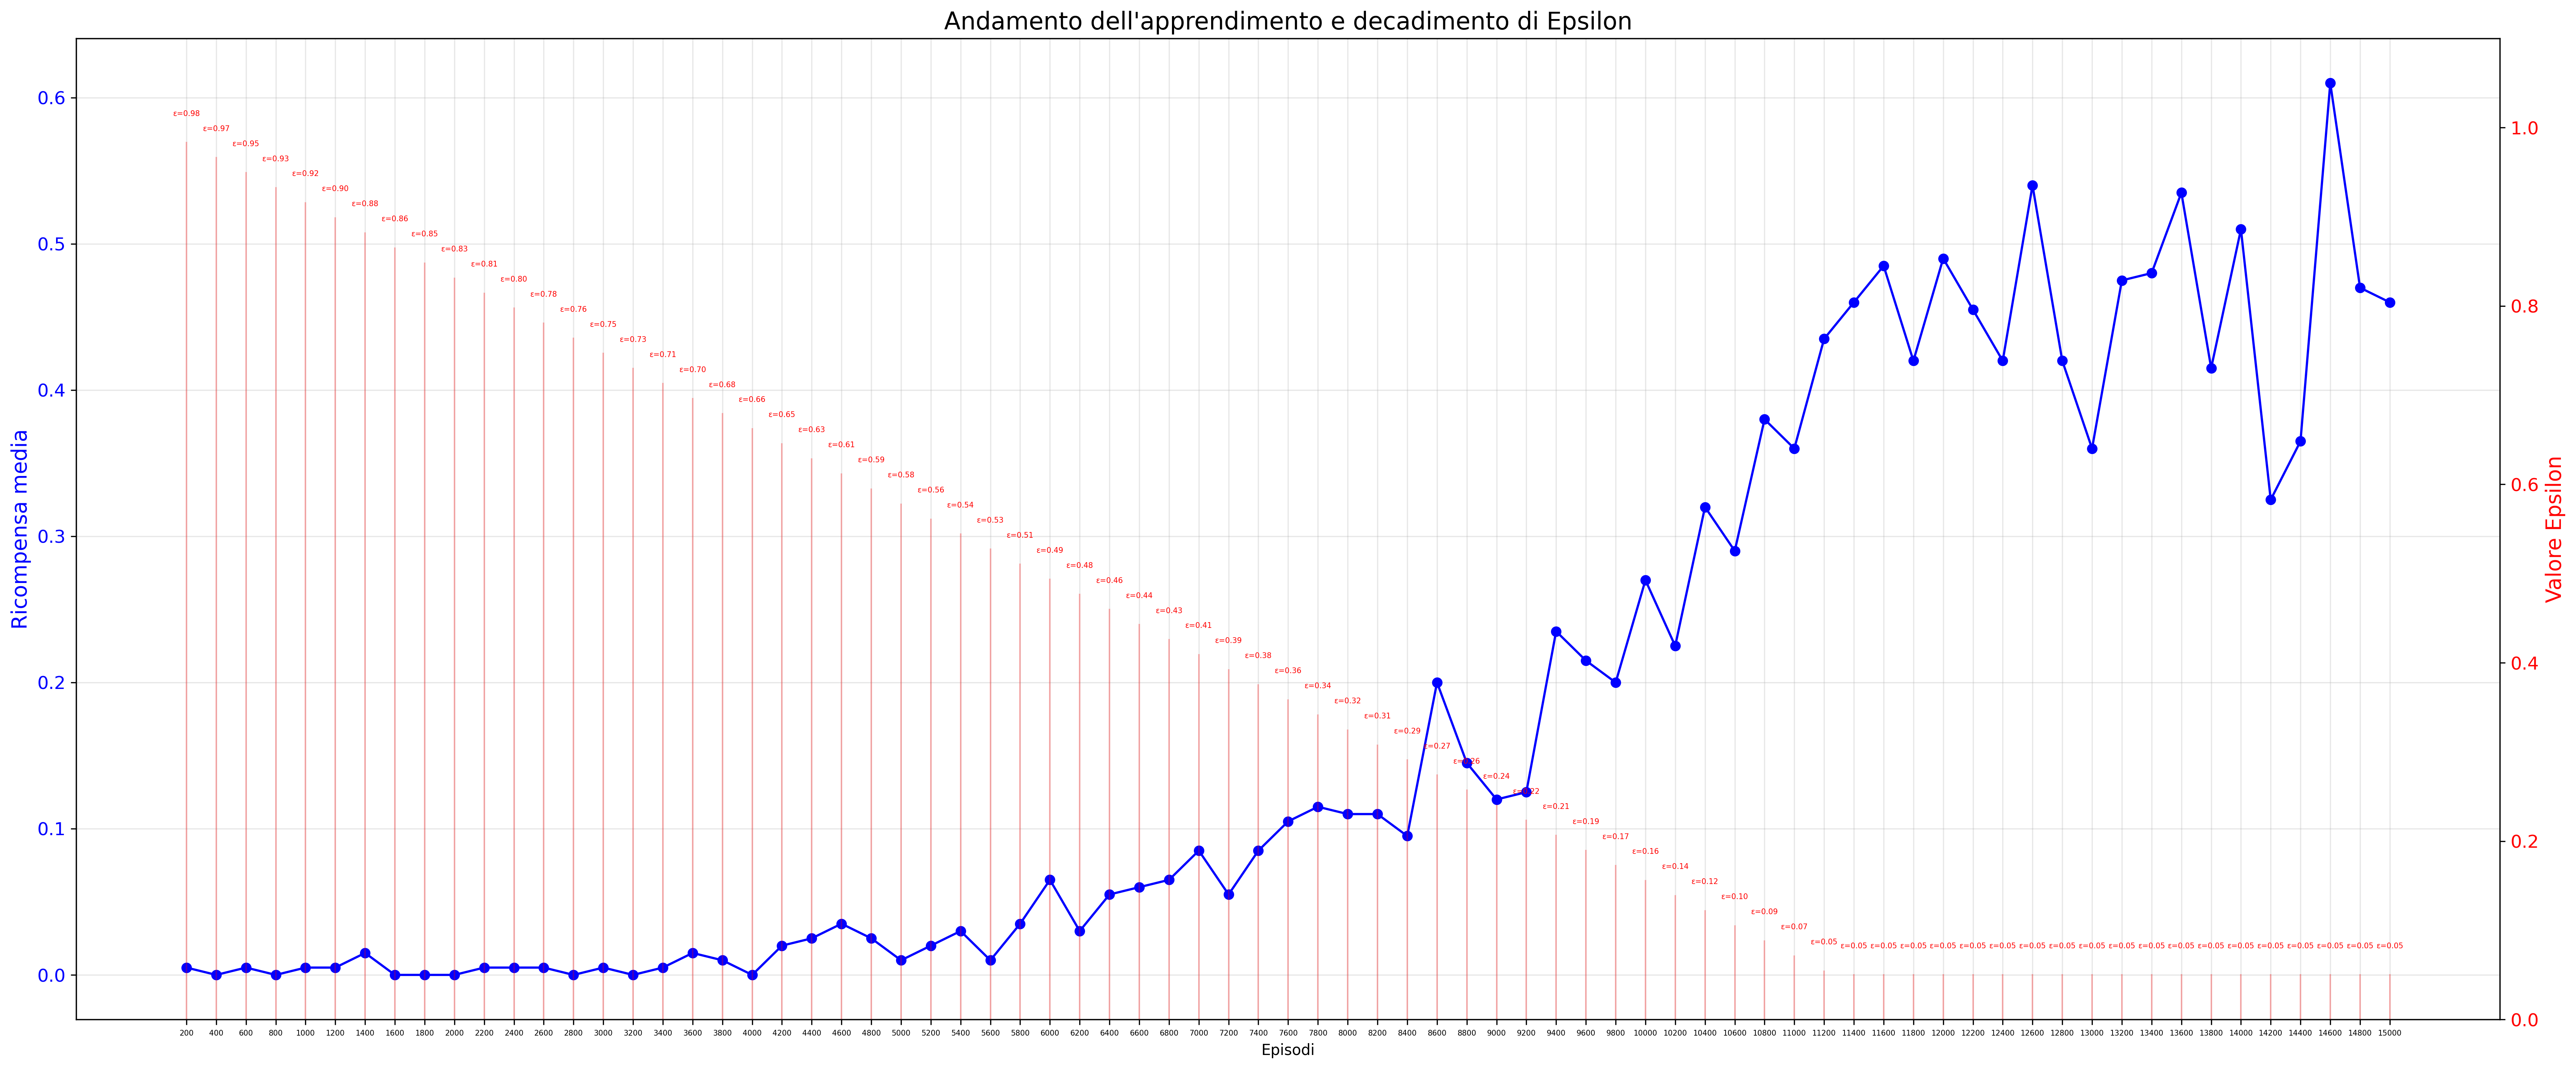
\includegraphics{TQL2;lr=0.1;nep=15000;eps=1.0;fineps=0.05;eps_dec=8.444444444444444e-05;gam=0.99.png}}
\end{center}


\begin{center}
\centering
\resizebox{\textwidth}{!}{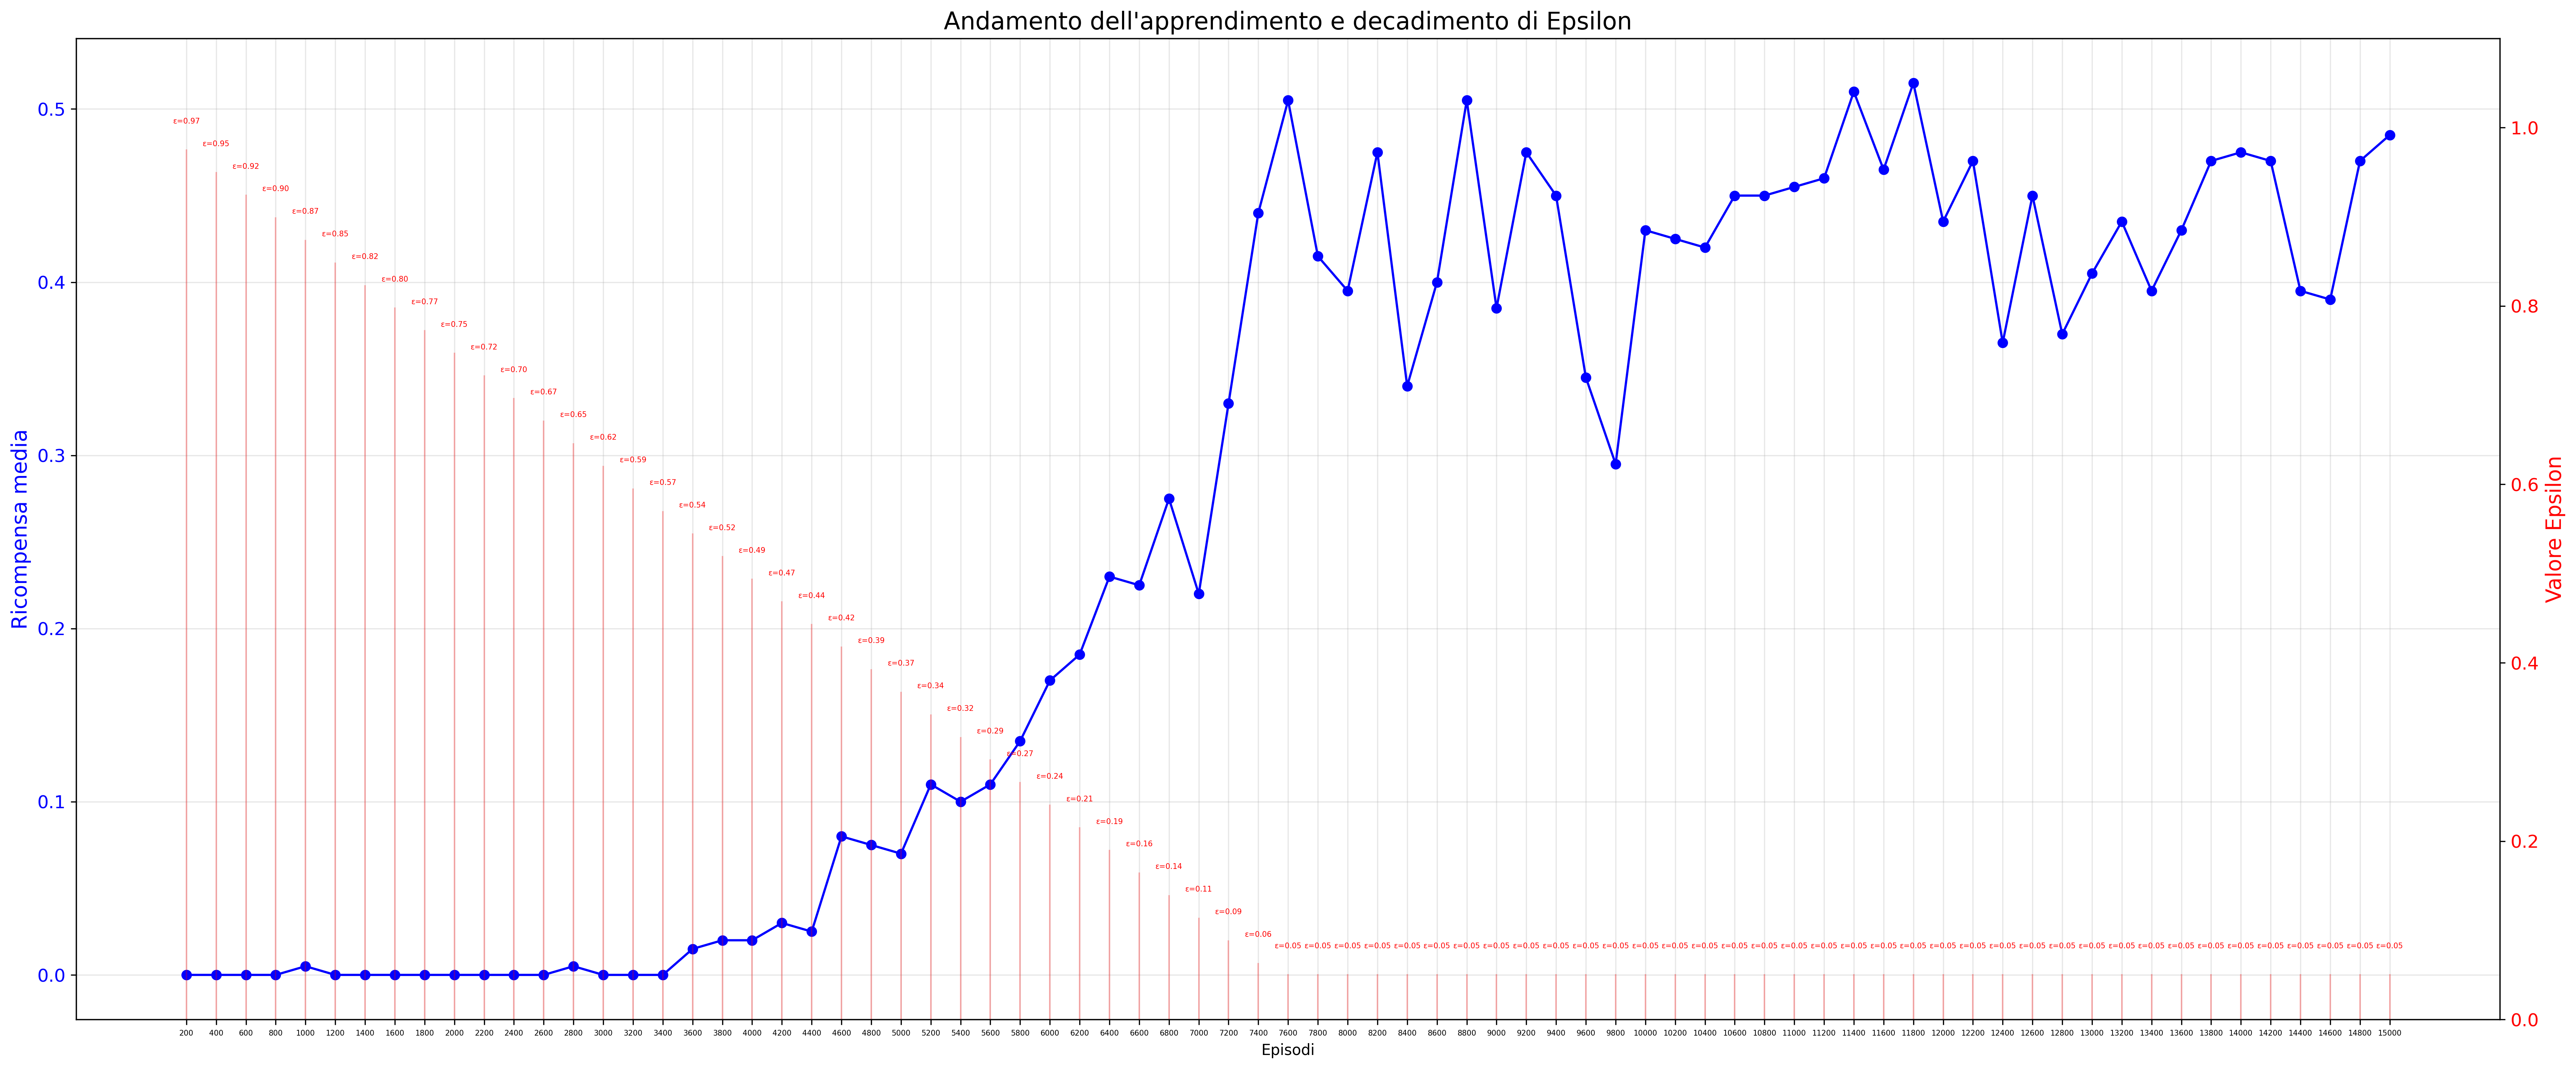
\includegraphics{TQL2;lr=0.1;nep=15000;eps=1.0;fineps=0.05;eps_dec=0.00012666666666666666;gam=0.99.png}}
\end{center}


Looking at the convergence time aspect, the second setting seems to be the only one that converges, doing so from episode 11200, while the other two do not seem to converge for different reasons:
\\
the first one starts entering the "exploitation" phase too late, although still showing a sort of settlement towards the final episodes.
\\
The third one, on the other hand, ends the "exploration" phase too early and indeed obtains null results when it tries to exploit the Q-table.
\\
In terms of average cumulative reward at convergence, again the second setting behaves in the best way, taking into account an average reward of 0.46.
\\
The first one also behaves goodly, bringing an average reward of 0.4; instead, the third setting behaves in the worst possible way, bringing a 0 reward.
\\
During the testing phase, those results are almost reflected, so, in 2000 test episodes, the first setting has a success rate of the 52.6\%, less worse that the second one, which has a success rate of the 53.4\%.
\\
Obviously, the third configuration has only a success rate of the 0.4\%.
\\
in conclusion, I would say that choosing a decay rate of value 8.44$\times10^{-5}$, is the best choice as analyzed previously.

\subsubsection{Changing the learning rate}

Now, I have choosen as decay rate, for evaluating the variation of the learning rates, of 8.44$\times10^{-5}$: so I can find almost the best settings in terms of decay rate and learning value.
\\
From the first plot to the third, the $\alpha$ value assumes the following values (as previously described):
\begin{itemize}
\item[--] The first sets $\alpha$ to 0.1
\item[--] The second sets $\alpha$ to 0.01
\item[--] The third sets $\alpha$ to 0.001
\end{itemize}

\clearpage


\begin{center}
\centering
\resizebox{\textwidth}{!}{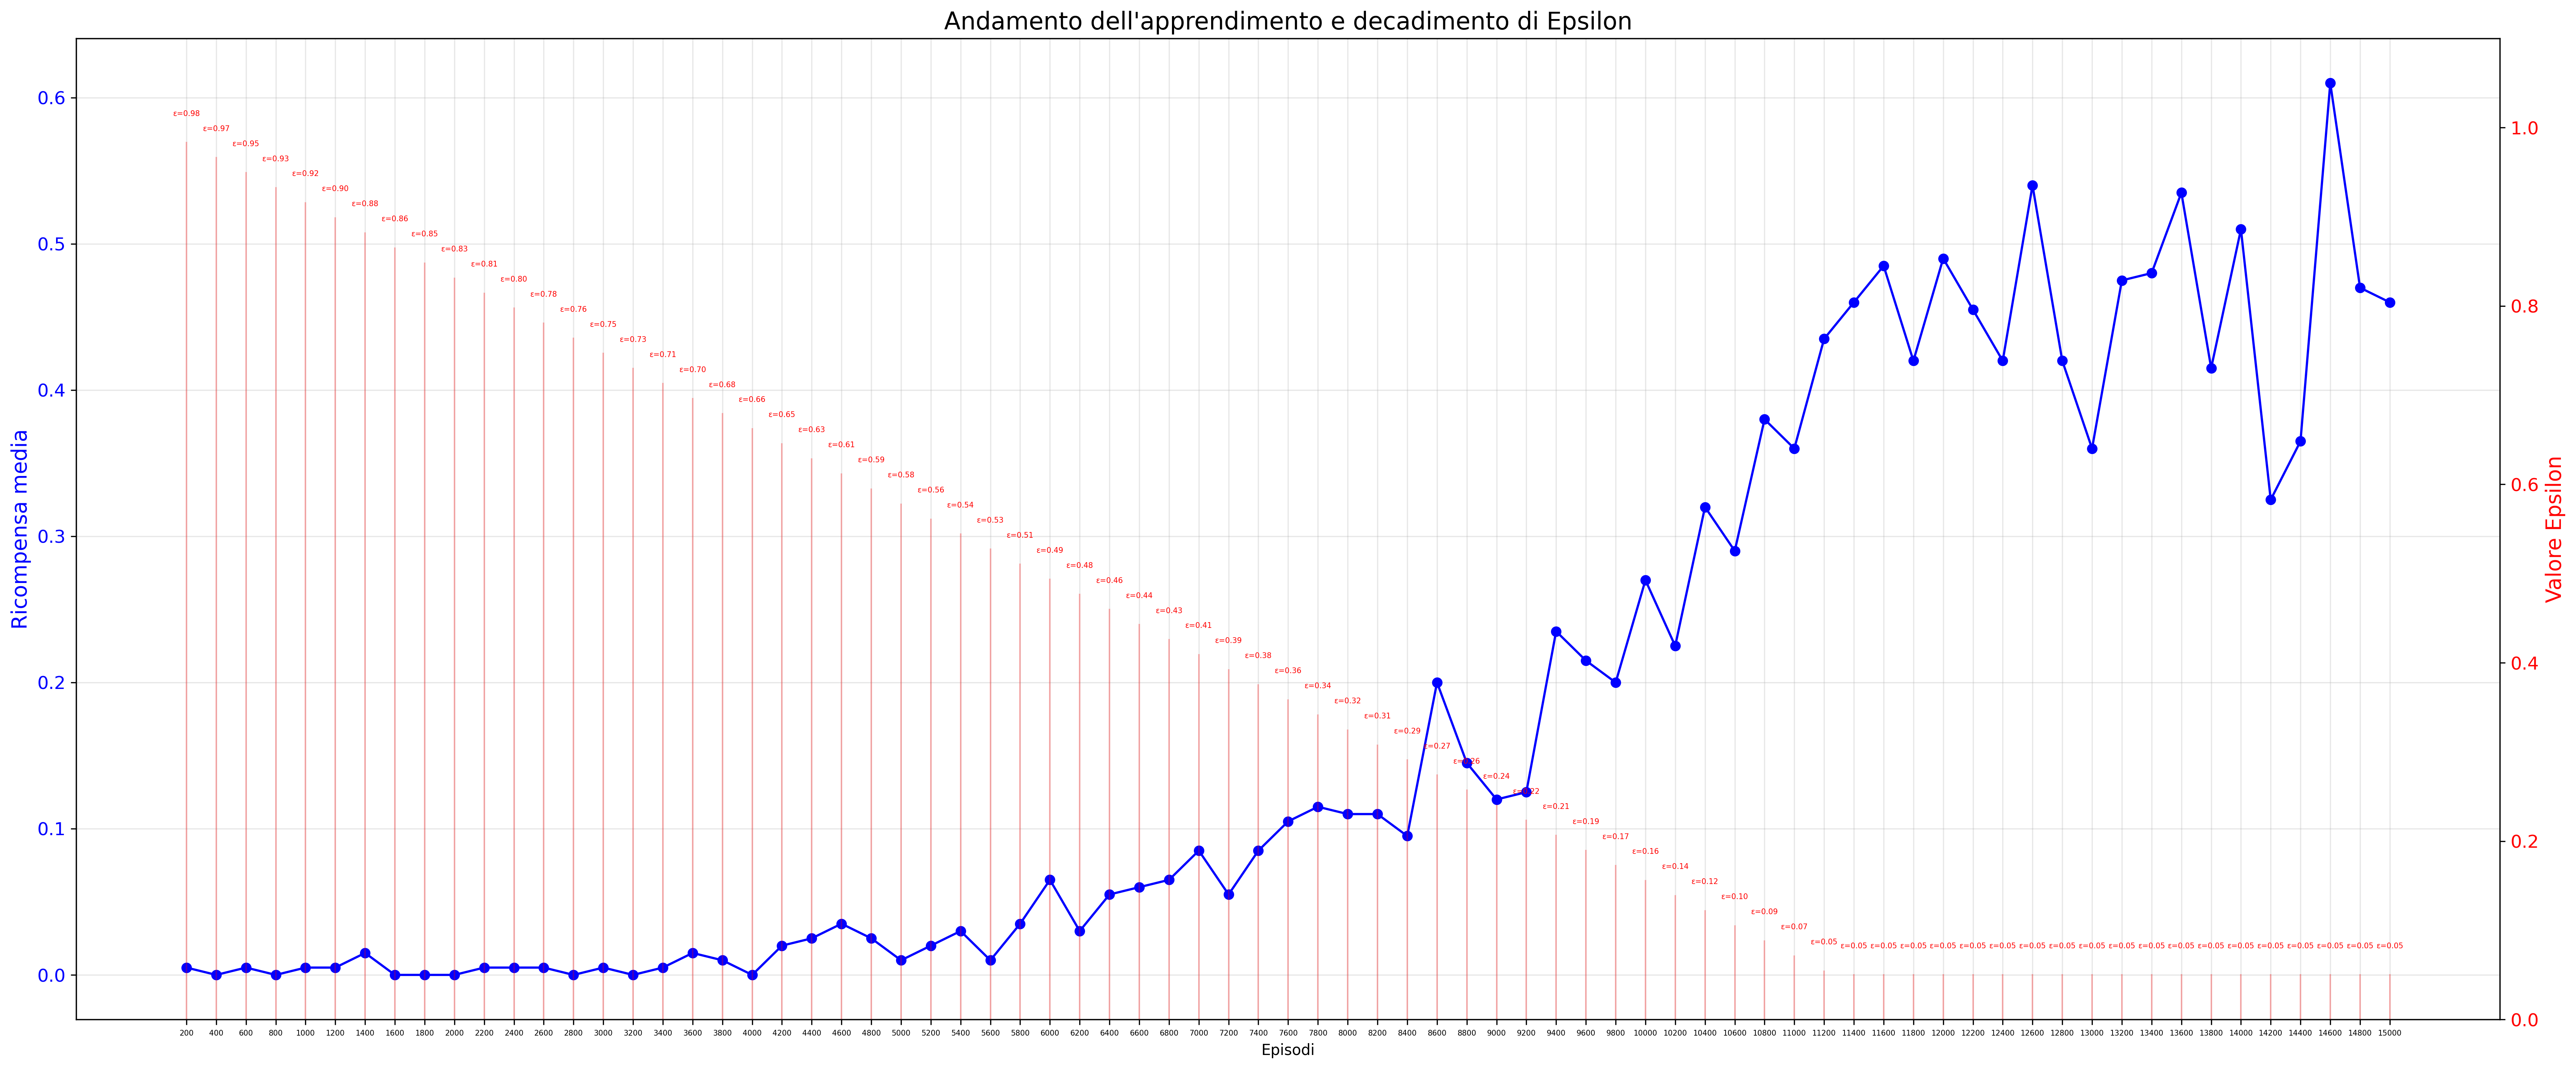
\includegraphics{TQL2;lr=0.1;nep=15000;eps=1.0;fineps=0.05;eps_dec=8.444444444444444e-05;gam=0.99.png}}
\end{center}

\begin{center}
\centering
\resizebox{\textwidth}{!}{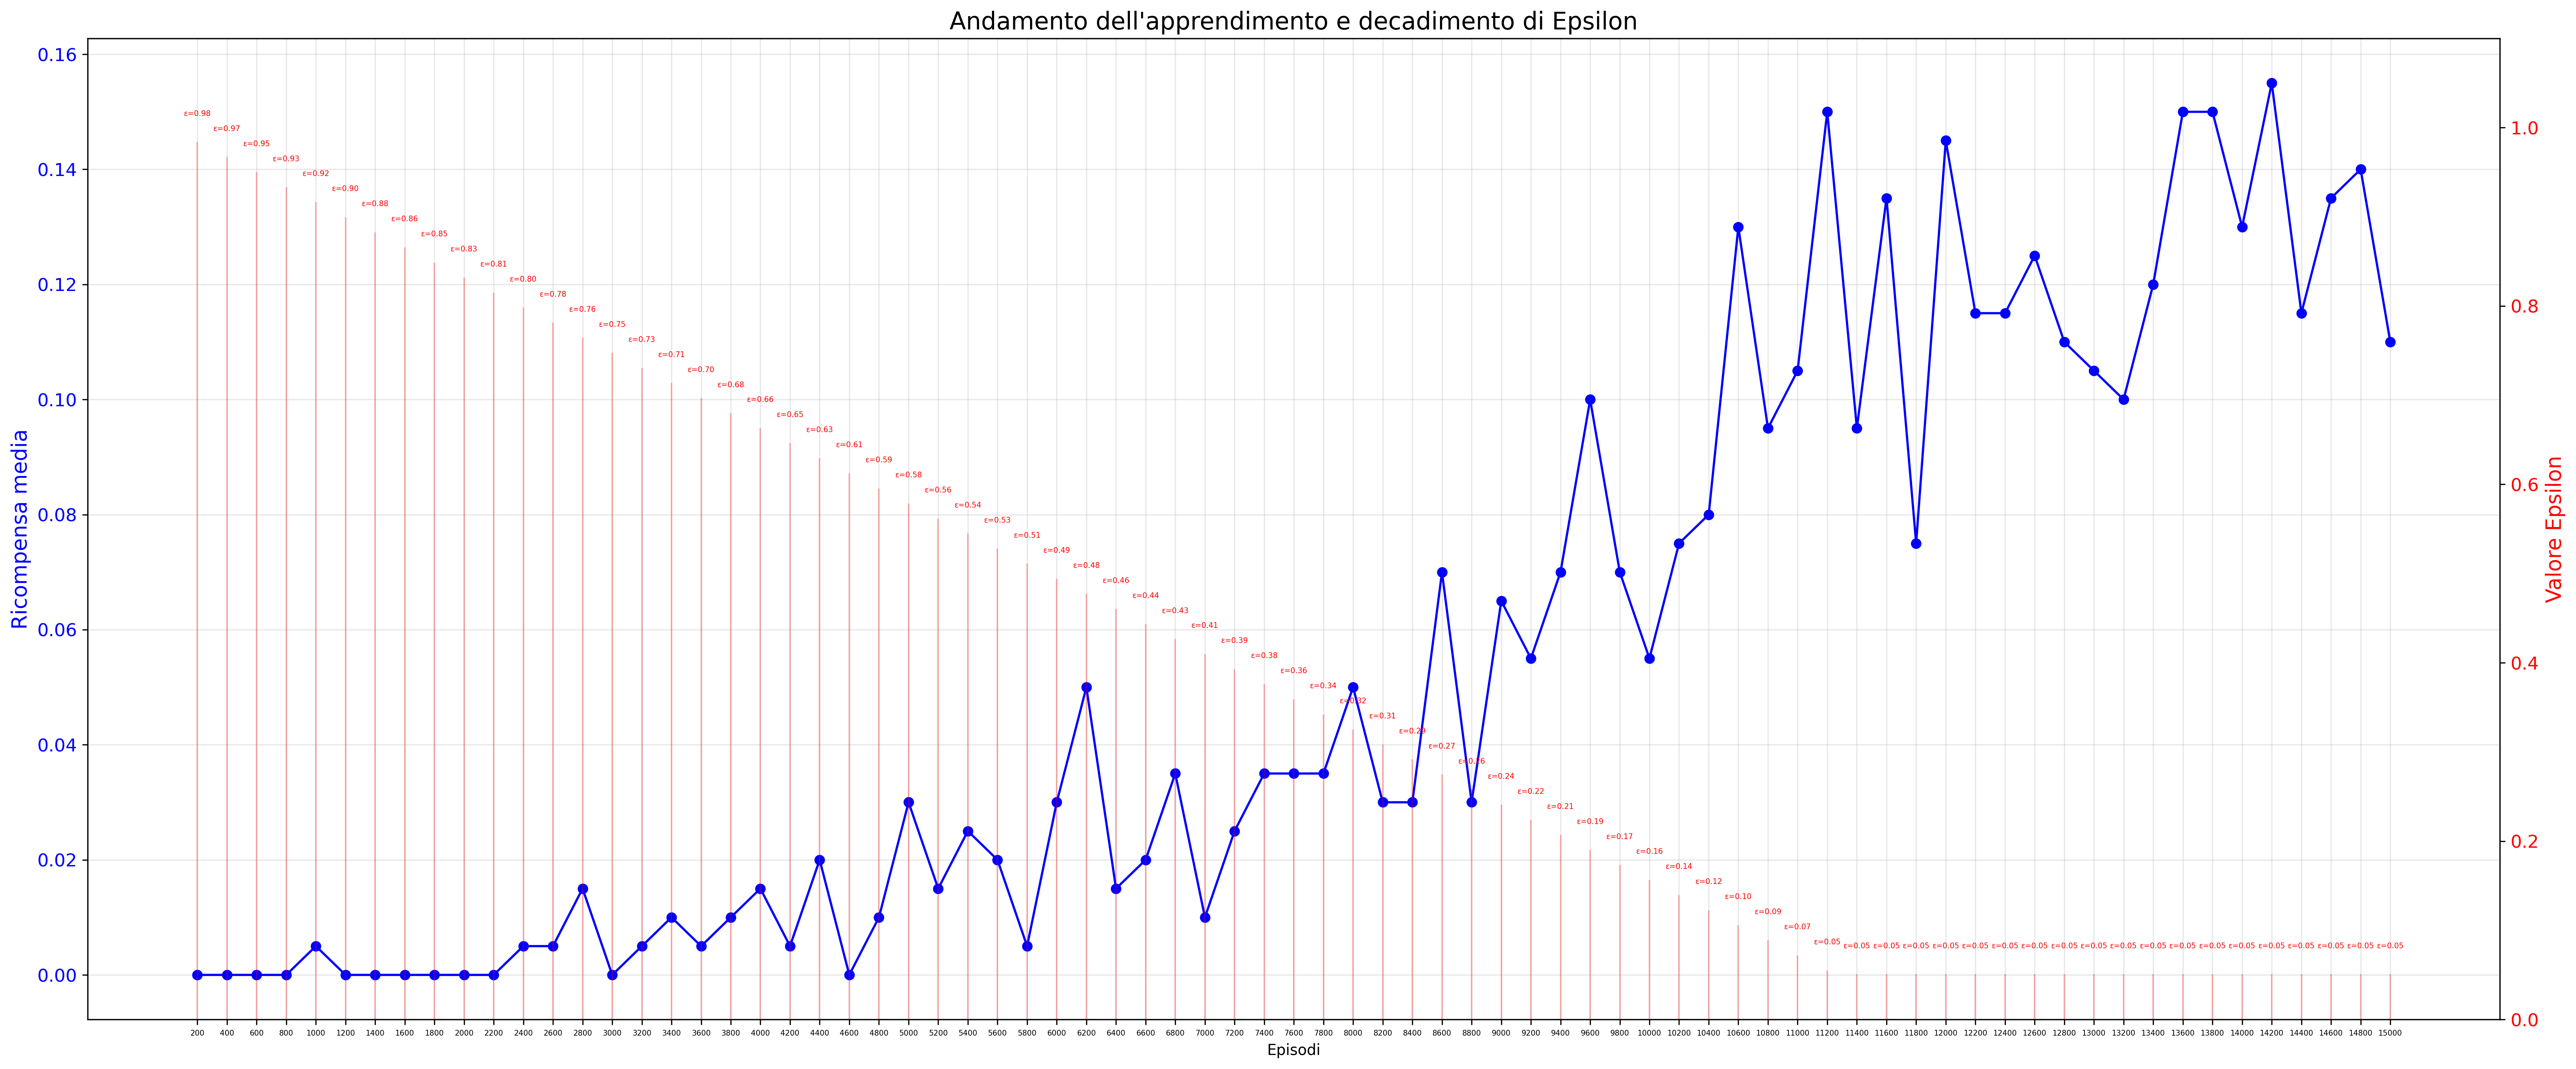
\includegraphics{TQL2;lr=0.01;nep=15000;eps=1.0;fineps=0.05;eps_dec=8.444444444444444e-05;gam=0.99.png}}
\end{center}

\begin{center}
\centering
\resizebox{\textwidth}{!}{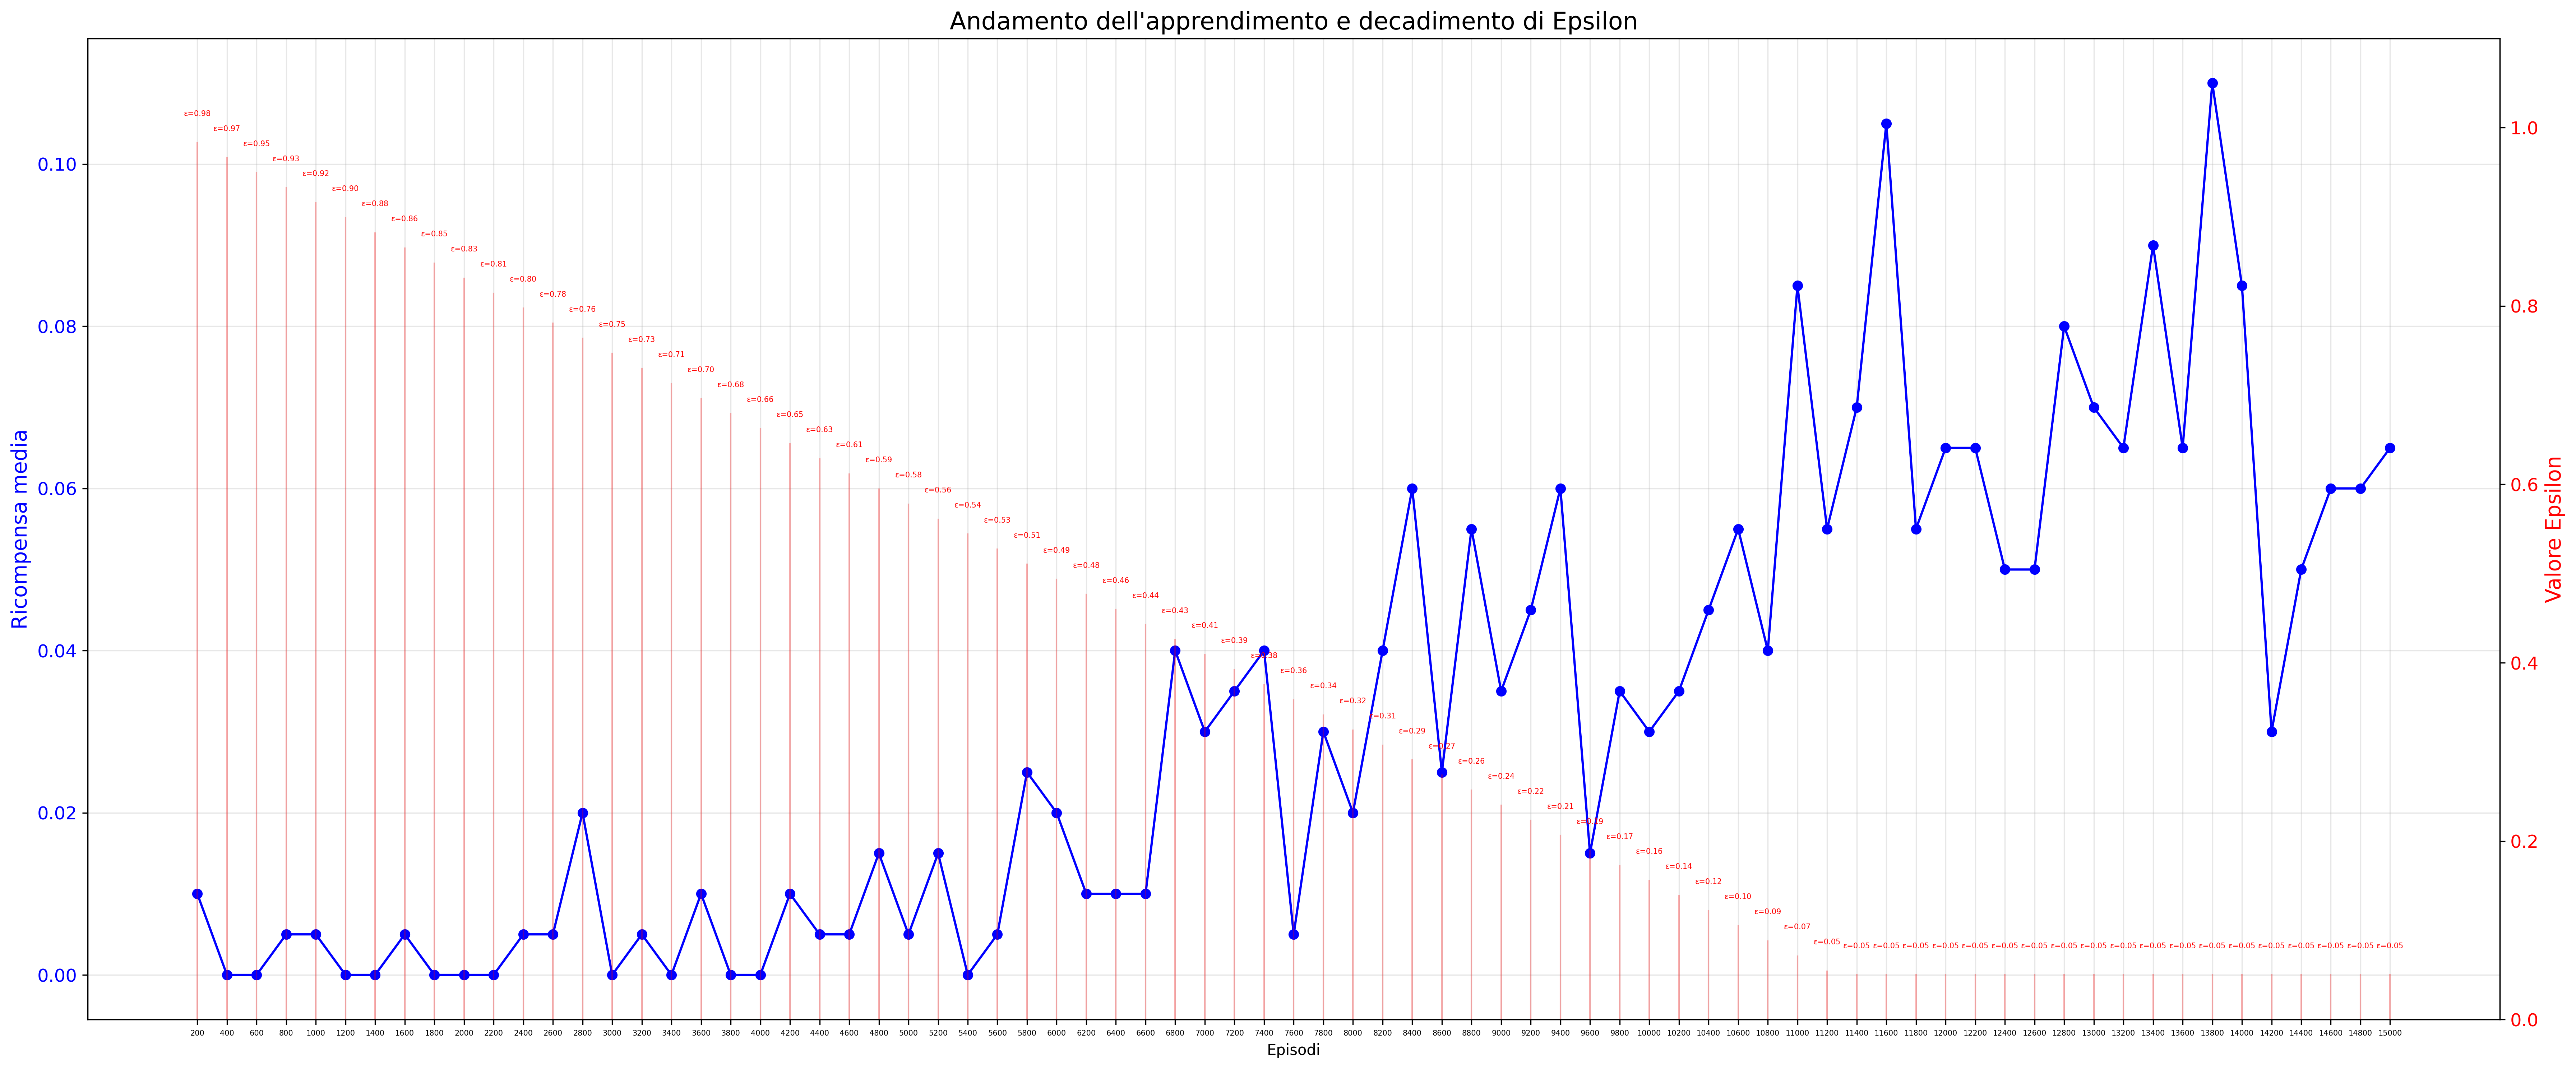
\includegraphics{TQL2;lr=0.001;nep=15000;eps=1.0;fineps=0.05;eps_dec=8.444444444444444e-05;gam=0.99.png}}
\end{center}

\clearpage

In terms of convergence time, having both the three solutions the same epsilon decay value, they did it almost near the same episodes (near 11000 episodes).
\\
The average cumulative reward argument is interesting cause, as the learning rate decreases, the cumulative reward itself decreases:
\\
In fact, the first configuration has an average cumulative reward of 0.46 (and so 53.4\% of success rate during the testing); instead, the second one has it of 0.12, bringing a success rate in testing of 13.2\%.
\\
The third one, as we expected, seems to converge with a reward of 0.07, having a success rate of 8.5\% during the testing phase.
\\
So, having a learning rate near to 0.1 is the best choice. 


\subsubsection{Conclusions}

So, in conclusion, I would say that in the case of Tabular Q-learning in a non deterministic environment, the best configuration found is the following one:


\begin{itemize}
\item[--] $\alpha$= 0.1
\item[--] $\epsilon$ decay= 8.44$\times10^{-5}$
\item[--] initial $\epsilon$ = 1
\item[--] final $\epsilon$ = 0.05
\item[--] gamma = 0.99
\end{itemize}

Bringing an average cumulative reward in the testing phase of 0.534 and converging in about 11400 episodes.

This is the policy obtained from the Q-table, which is the best one:
\begin{center}
    \centering
    \resizebox{\textwidth}{!}{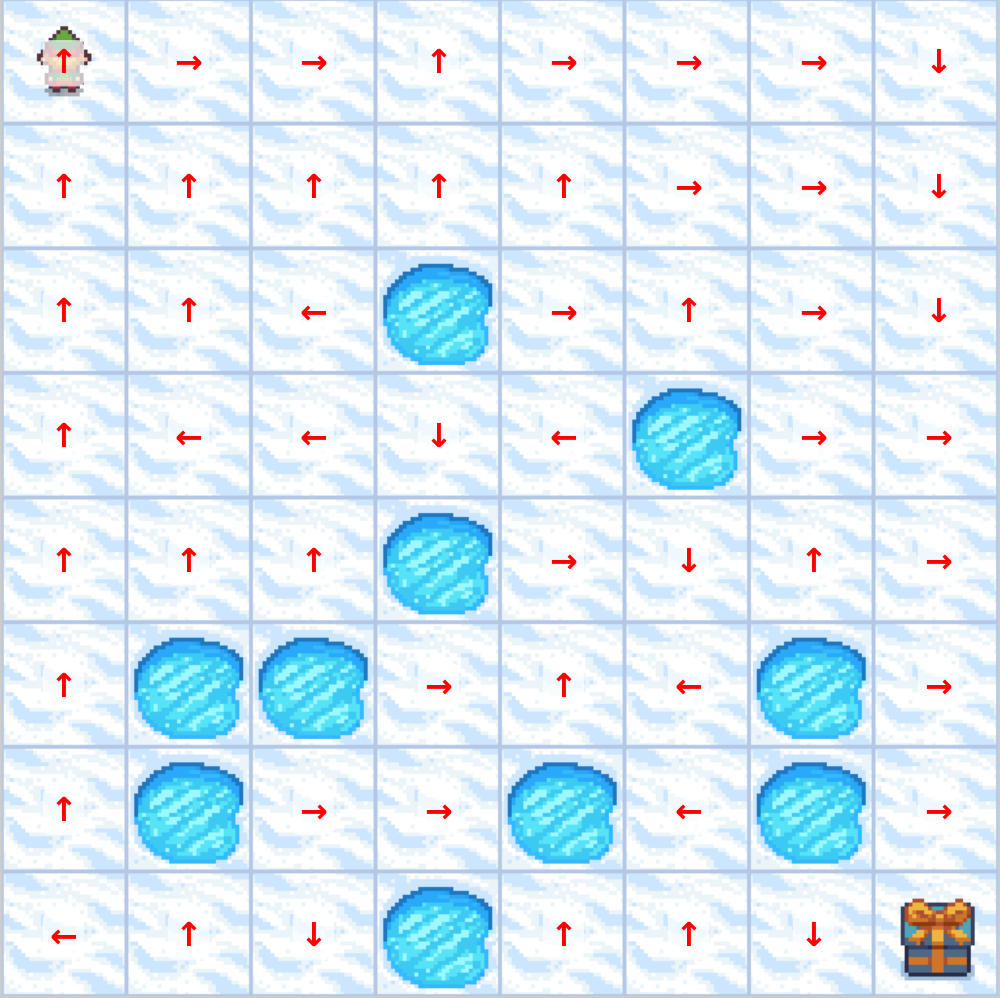
\includegraphics{policy_arrows_8x8.png}}
\end{center}

\section{Deep Q Network}

\subsection{Solution adopted}

\begin{figure}[h]
    \centering
    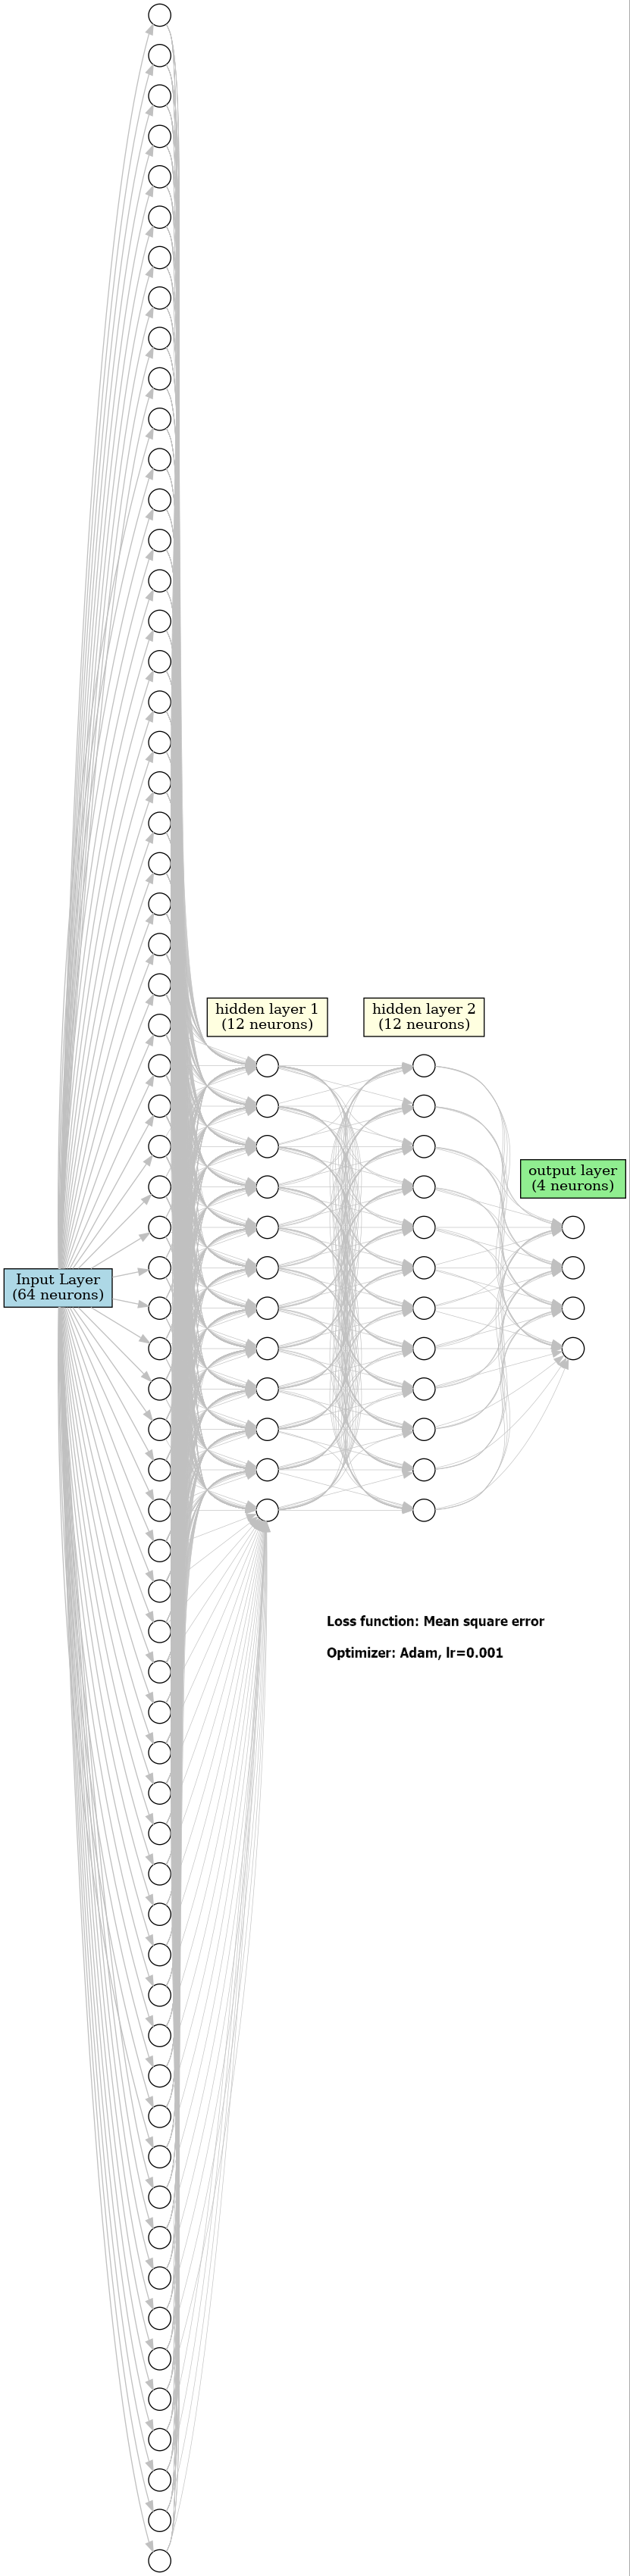
\includegraphics[height=\textheight]{NN_architecture2.png}
    \label{fig:nn_architecture}
\end{figure}
\clearpage

I have used tensorflow with keras for bulding a feedforward neural network for solving the Frozen Lake environment, using always the non deterministic Q learning technique.
\\
These are the characteristics of the network:
\begin{itemize}
\item[--] Feedforward neural network
\item[--] Width is 64, cause the number of neurons of the input layer
\item[--] Depth is 2, because we have 2 hidden layers
\item[--] The neurons are fully connected in a Dense way (each neuron is connected with all the following neurons)
\item[--] The activation function of the hidden layers is the Relu (Rectified linear units)
\item[--] The activation function of the output layer is the Linear (Identity function)
\item[--] The loss function used is the Mean Square Error
\item[--] The optimizer used is Adam, with a learning rate of 0.001
\item[--] The number of training episode is 15000
\item[--] The average cumulative reward is calculated over a range of 200 episodes
\item[--] The number of test episodes is 2000
\item[--] The mini-batch size is 64
\end{itemize}





The number of neurons in the neural network, and the type of connection (Dense), achieves the presence of 960 weight parameters.

\subsection{Metric results}


\subsubsection{Changing the epsilon decay}


These are the common hyper parameters for the runs (which are the same as previous):
\begin{itemize}
\item[--] $\alpha$= 0.1
\item[--] initial $\epsilon$ = 1
\item[--] final $\epsilon$ = 0.05
\item[--] gamma = 0.99
\end{itemize}

From the first plot to the third, the $\epsilon$ decay rate is increased as follows:

\begin{itemize}
\item[--] The first brings $\epsilon$ to its minimum value at 7/8 of the episodes.
\item[--] The second brings $\epsilon$ to the minimum at 3/4 of the episodes.
\item[--] The last one brings $\epsilon$ to the minimum at 1/2 of the total episodes.
\end{itemize}


\begin{center}
\centering
\resizebox{\textwidth}{!}{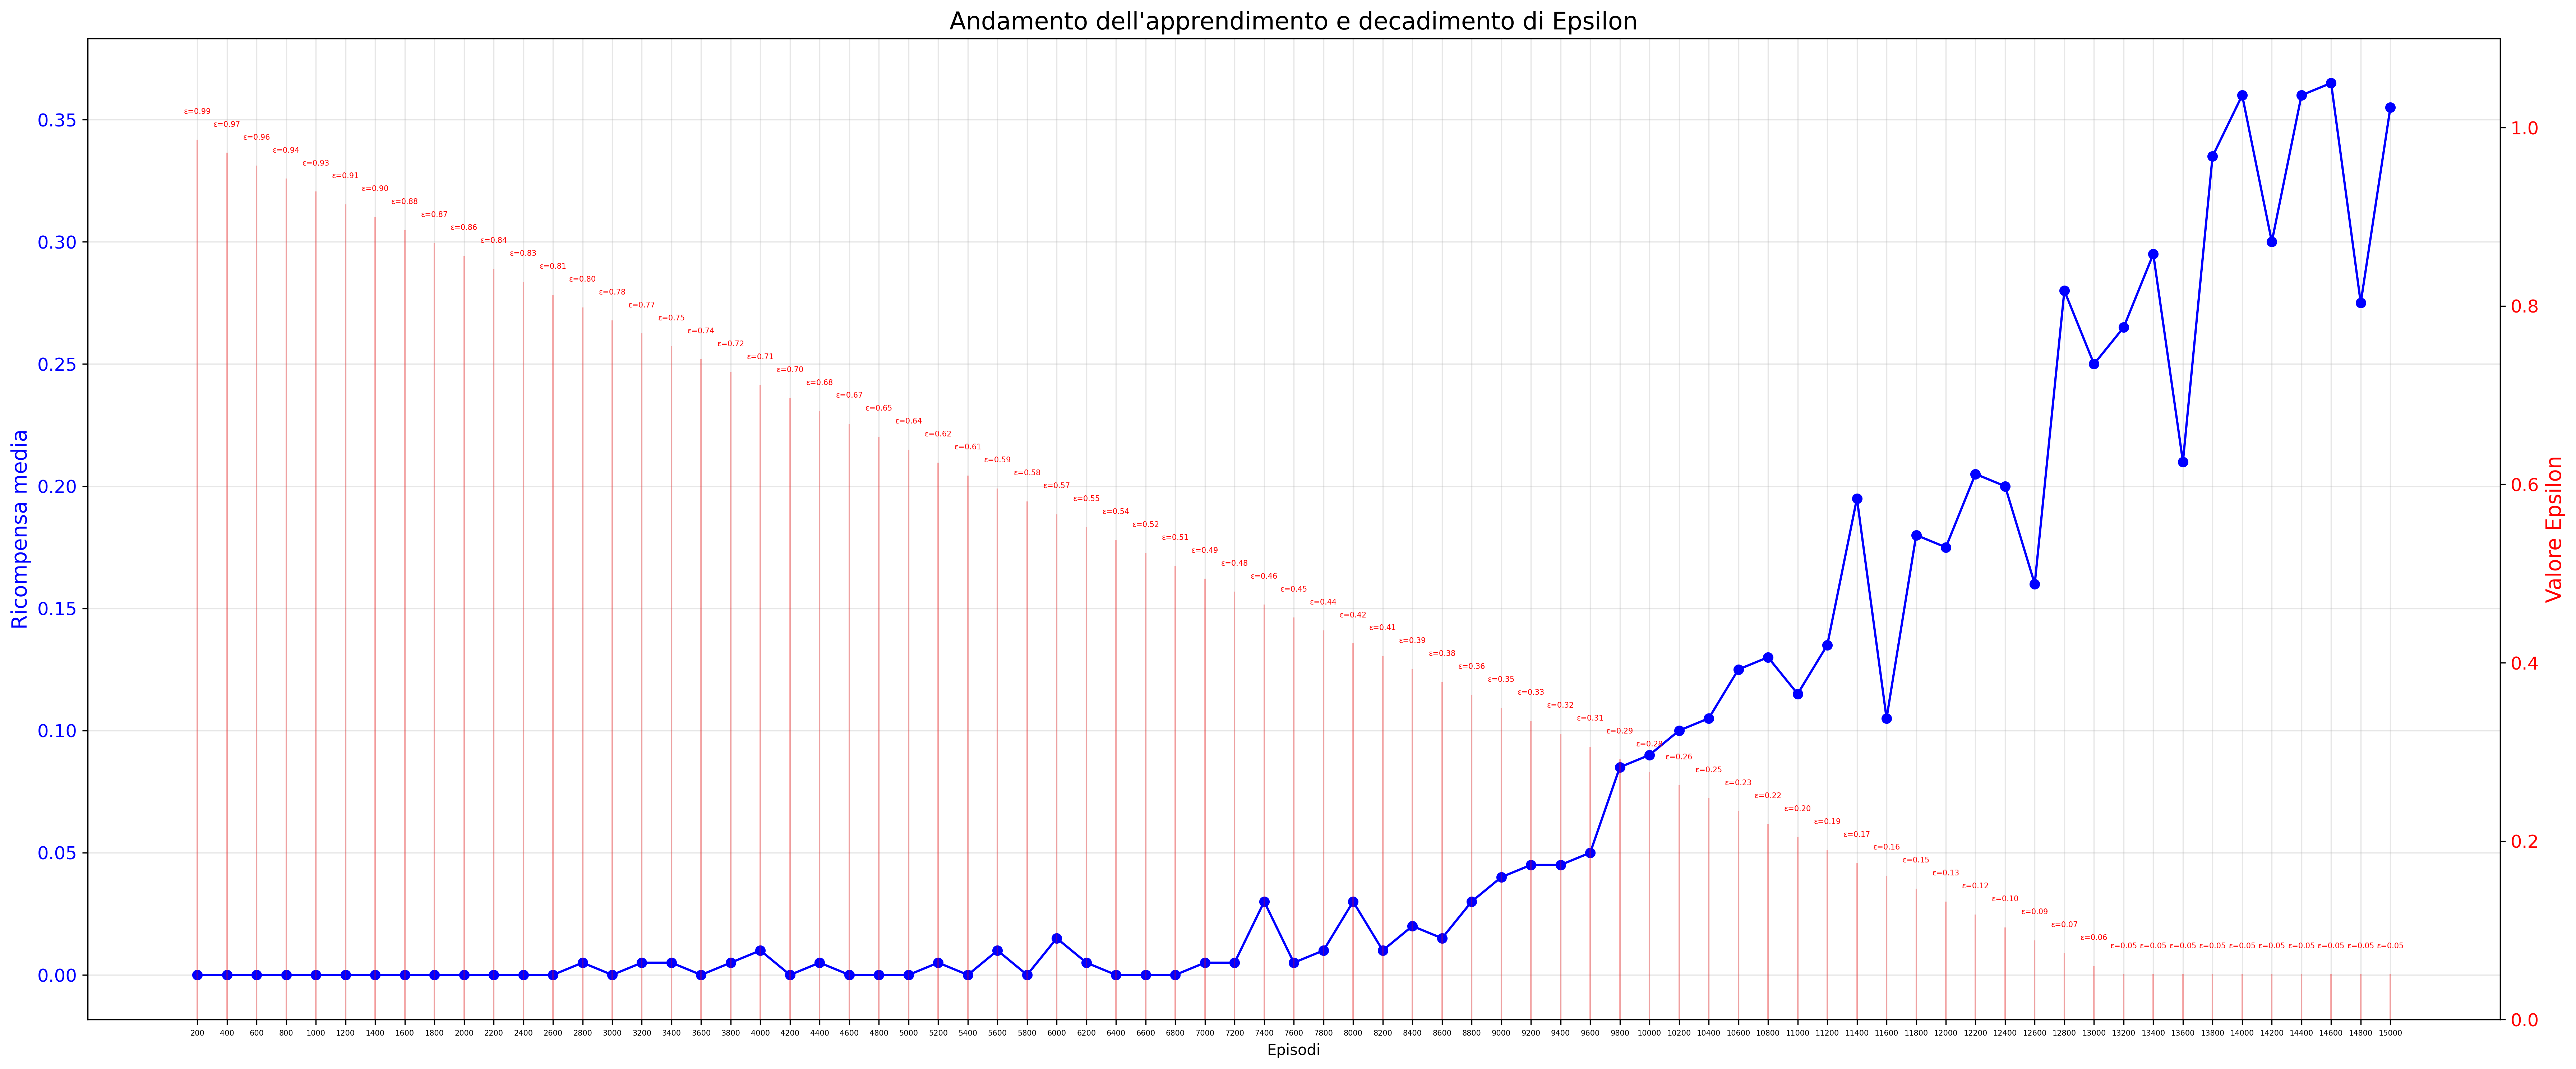
\includegraphics{DQN2;lr=0.1;nep=15000;eps=1.0;fineps=0.05;eps_dec=7.238095238095238e-05;gam=0.99.png}}
\end{center}

\begin{center}
\centering
\resizebox{\textwidth}{!}{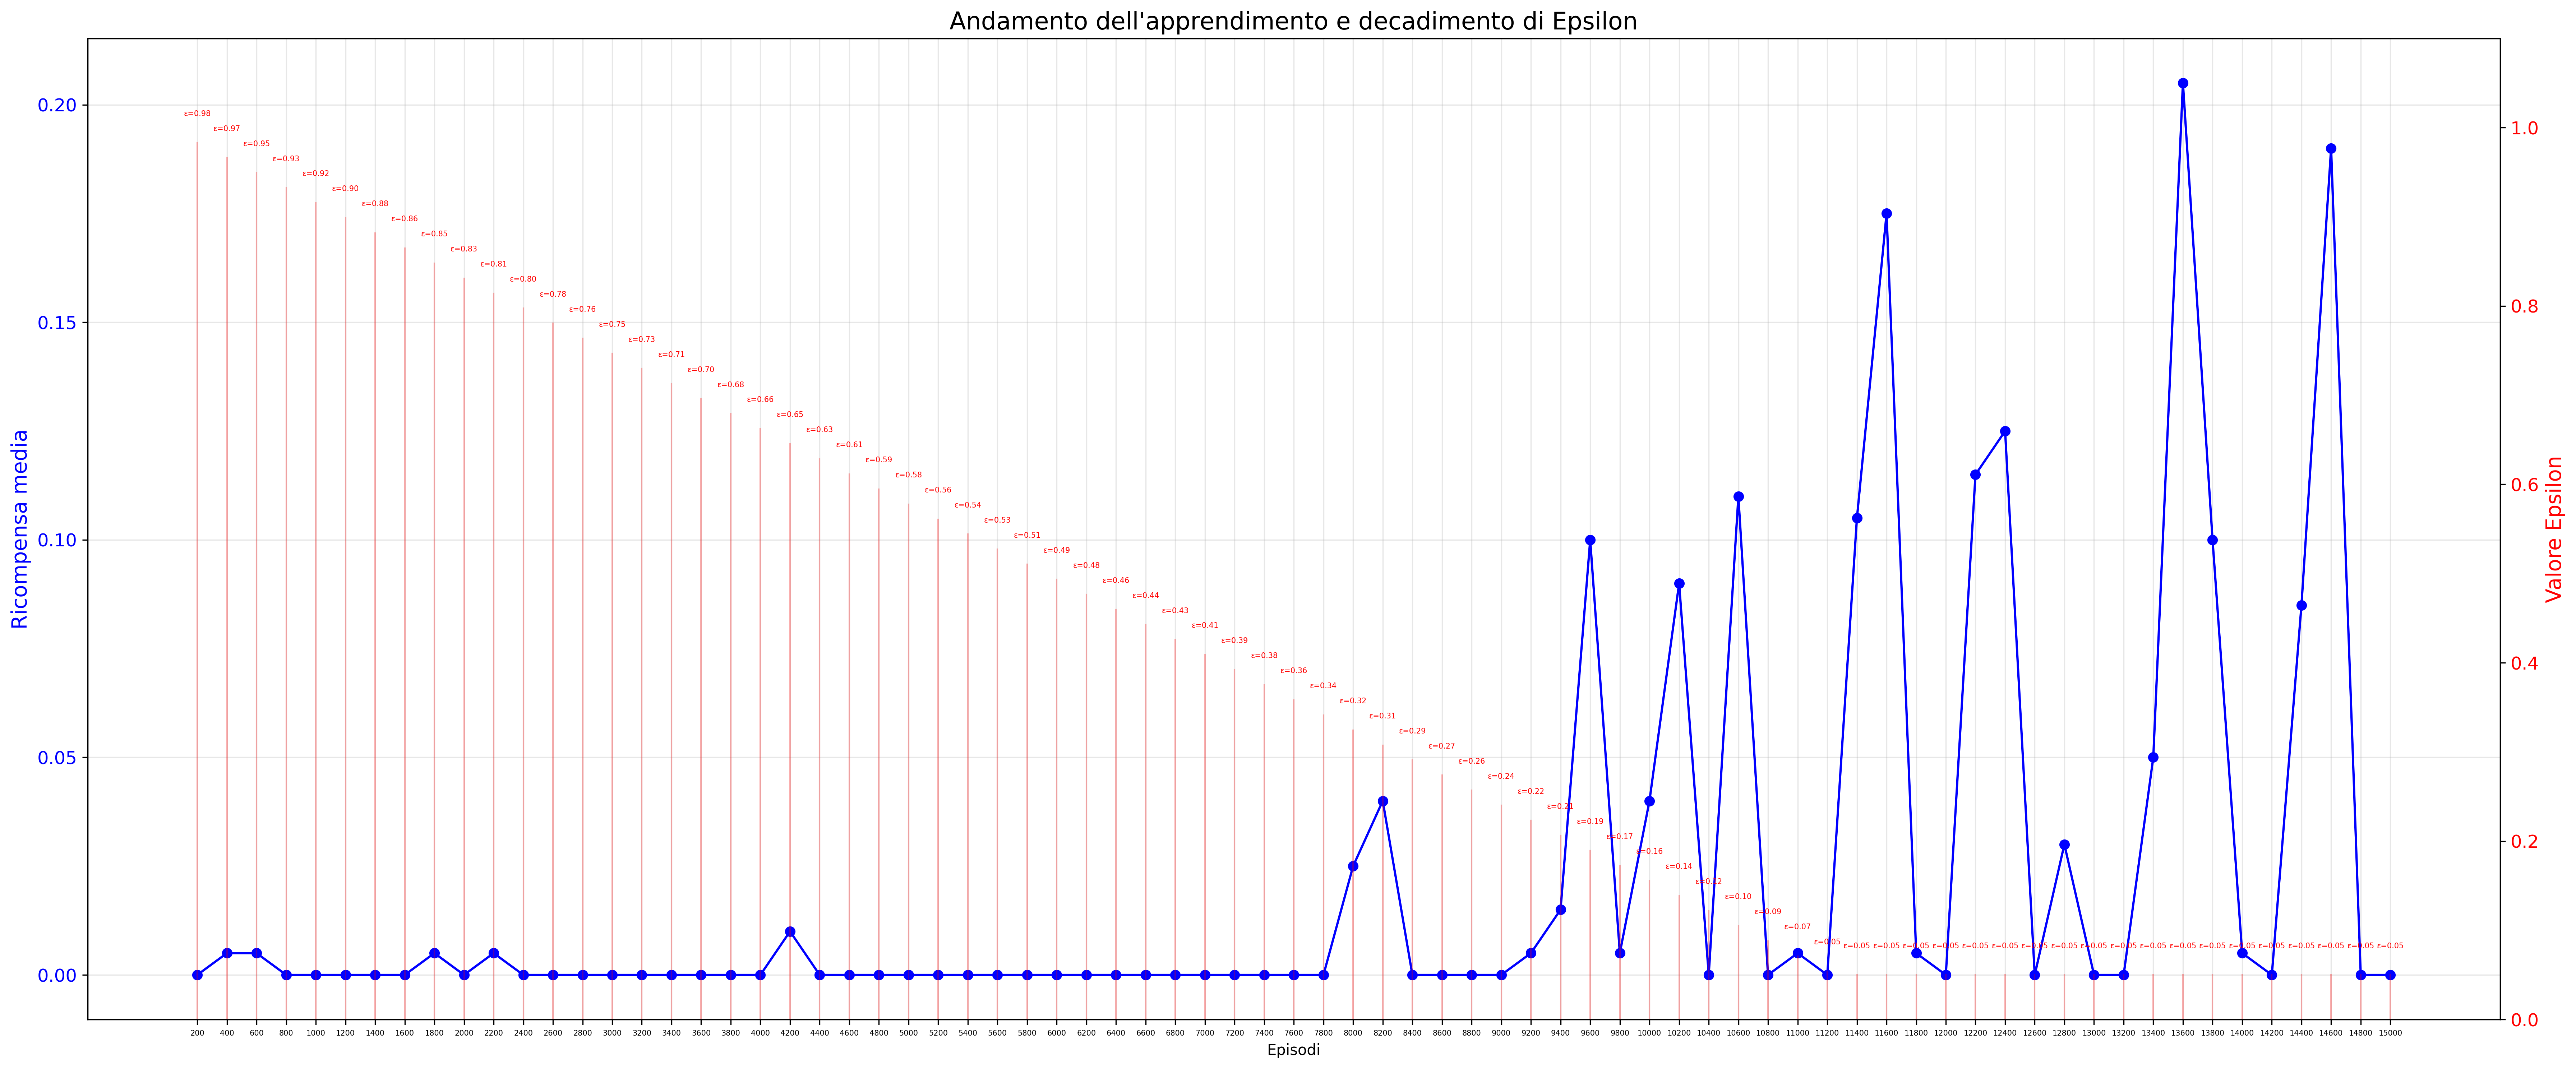
\includegraphics{DQN2;lr=0.1;nep=15000;eps=1.0;fineps=0.05;eps_dec=8.444444444444444e-05;gam=0.99.png}}
\end{center}

\begin{center}
\centering
\resizebox{\textwidth}{!}{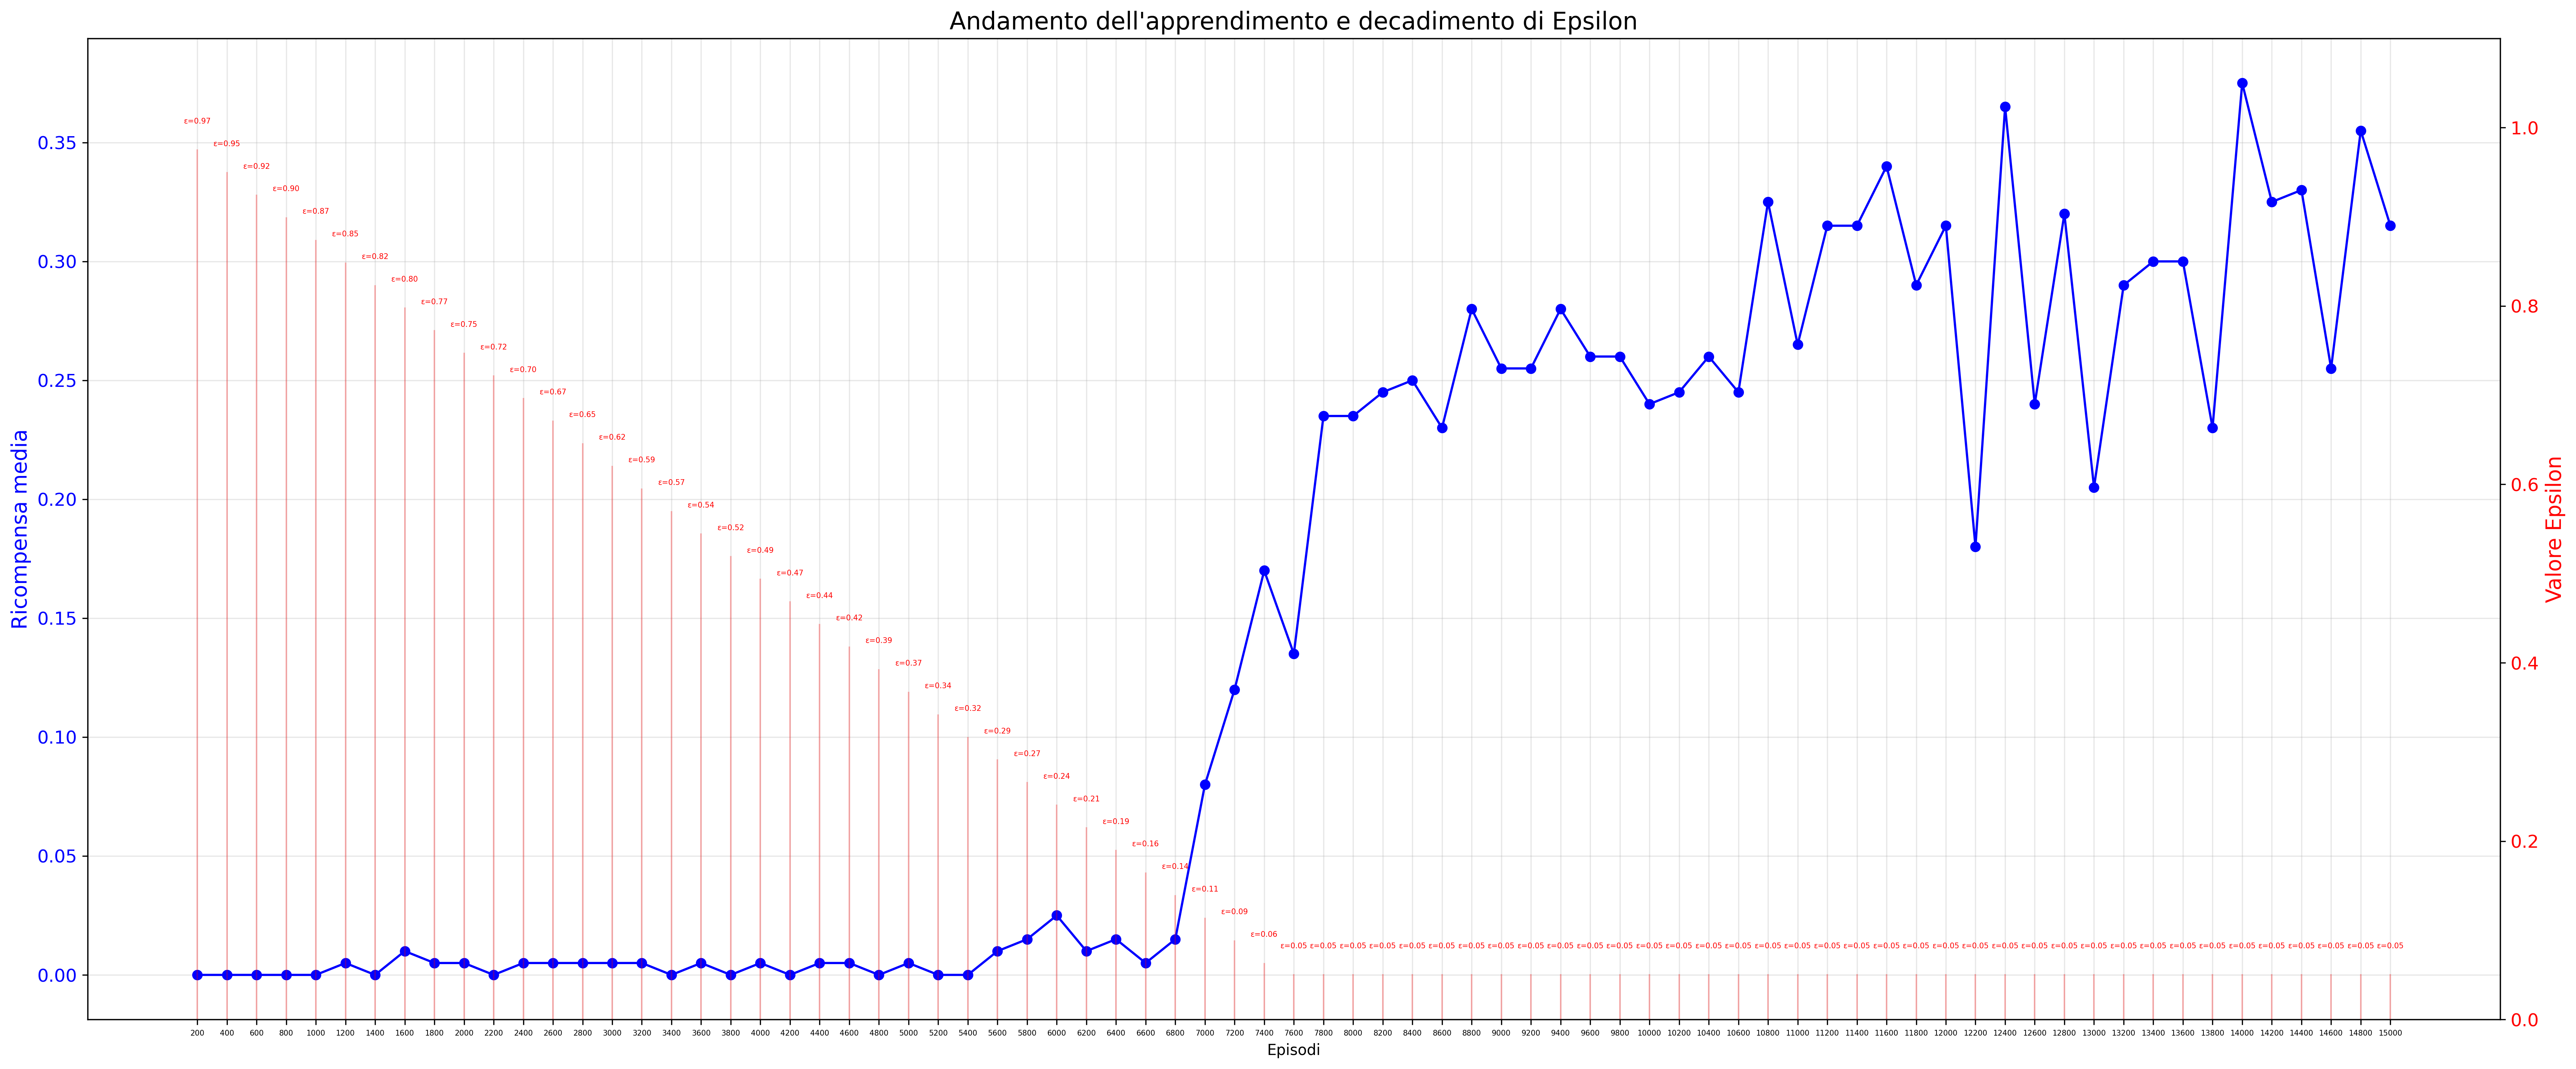
\includegraphics{DQN2;lr=0.1;nep=15000;eps=1.0;fineps=0.05;eps_dec=0.00012666666666666666;gam=0.99.png}}
\end{center}

\clearpage

In the first configuration the convergence is achieved near at 13200 episodes, then the second one converges at 11400 and, instead, the third one near 7800.
If we focus on the average cumulative reward at convergence, we could say that the third setting is the best, bringing a value of 0.27 and with a success rate in the testing phase of 45.2\%.
\\
Furthermore, the second configuration has similar performances in terms of average cumulative reward, with respect to the third one, bringing a value of 0.27 and a success rate of 44.6\% over the 2000 test episodes.
\\
Finally, the first configuration also seems to bring an average reward of value 0.28, but only a success rate of the 39.2\%.

I have noticed that, with different values, the conclusion is almost the same with respect of using the 4x4 map: in fact, we can conclude that, in terms of cumulative rewards, all the three possibilities has slightly the same performances:
\\
for this reason, as the best choice of configuration, I would pick the third one, cause is faster convergence.




\subsubsection{Changing the learning rate}


These are the common hyper parameters for the runs:
\begin{itemize}
\item[--] $\epsilon$ decay= 8.44$\times10^{-5}$
\item[--] initial $\epsilon$ = 1
\item[--] final $\epsilon$ = 0.05
\item[--] gamma = 0.99
\end{itemize}

From the first plot to the third, the $\alpha$ value assumes the following values :
\begin{itemize}
\item[--] The first sets $\alpha$ to 0.1
\item[--] The second sets $\alpha$ to 0.01
\item[--] The third sets $\alpha$ to 0.001
\end{itemize}

\clearpage


\begin{center}
\centering
\resizebox{\textwidth}{!}{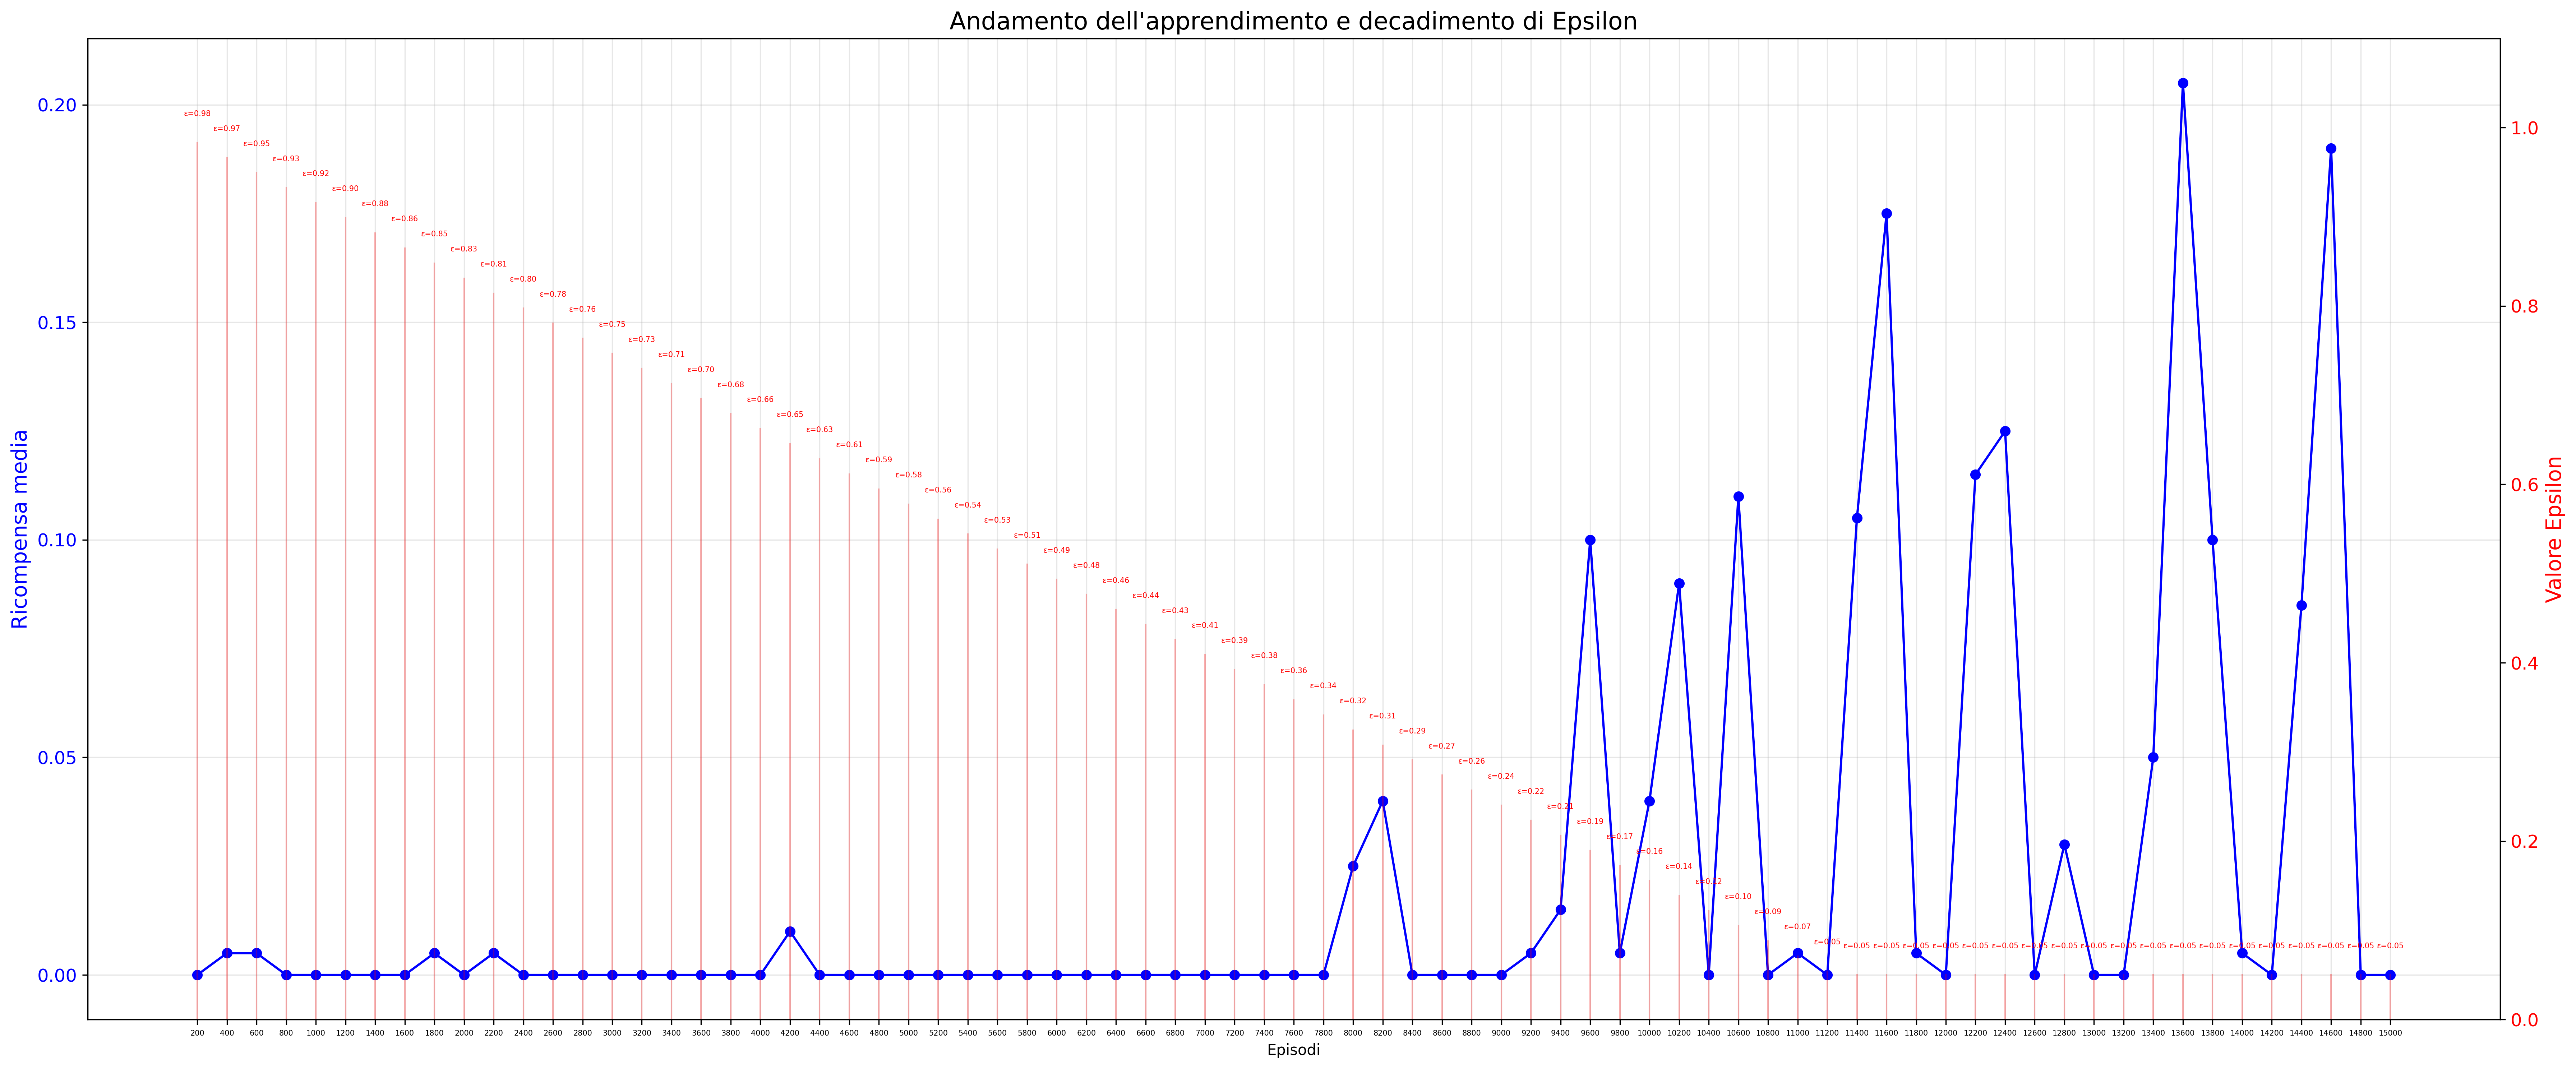
\includegraphics{DQN2;lr=0.1;nep=15000;eps=1.0;fineps=0.05;eps_dec=8.444444444444444e-05;gam=0.99.png}}
\end{center}

\begin{center}
\centering
\resizebox{\textwidth}{!}{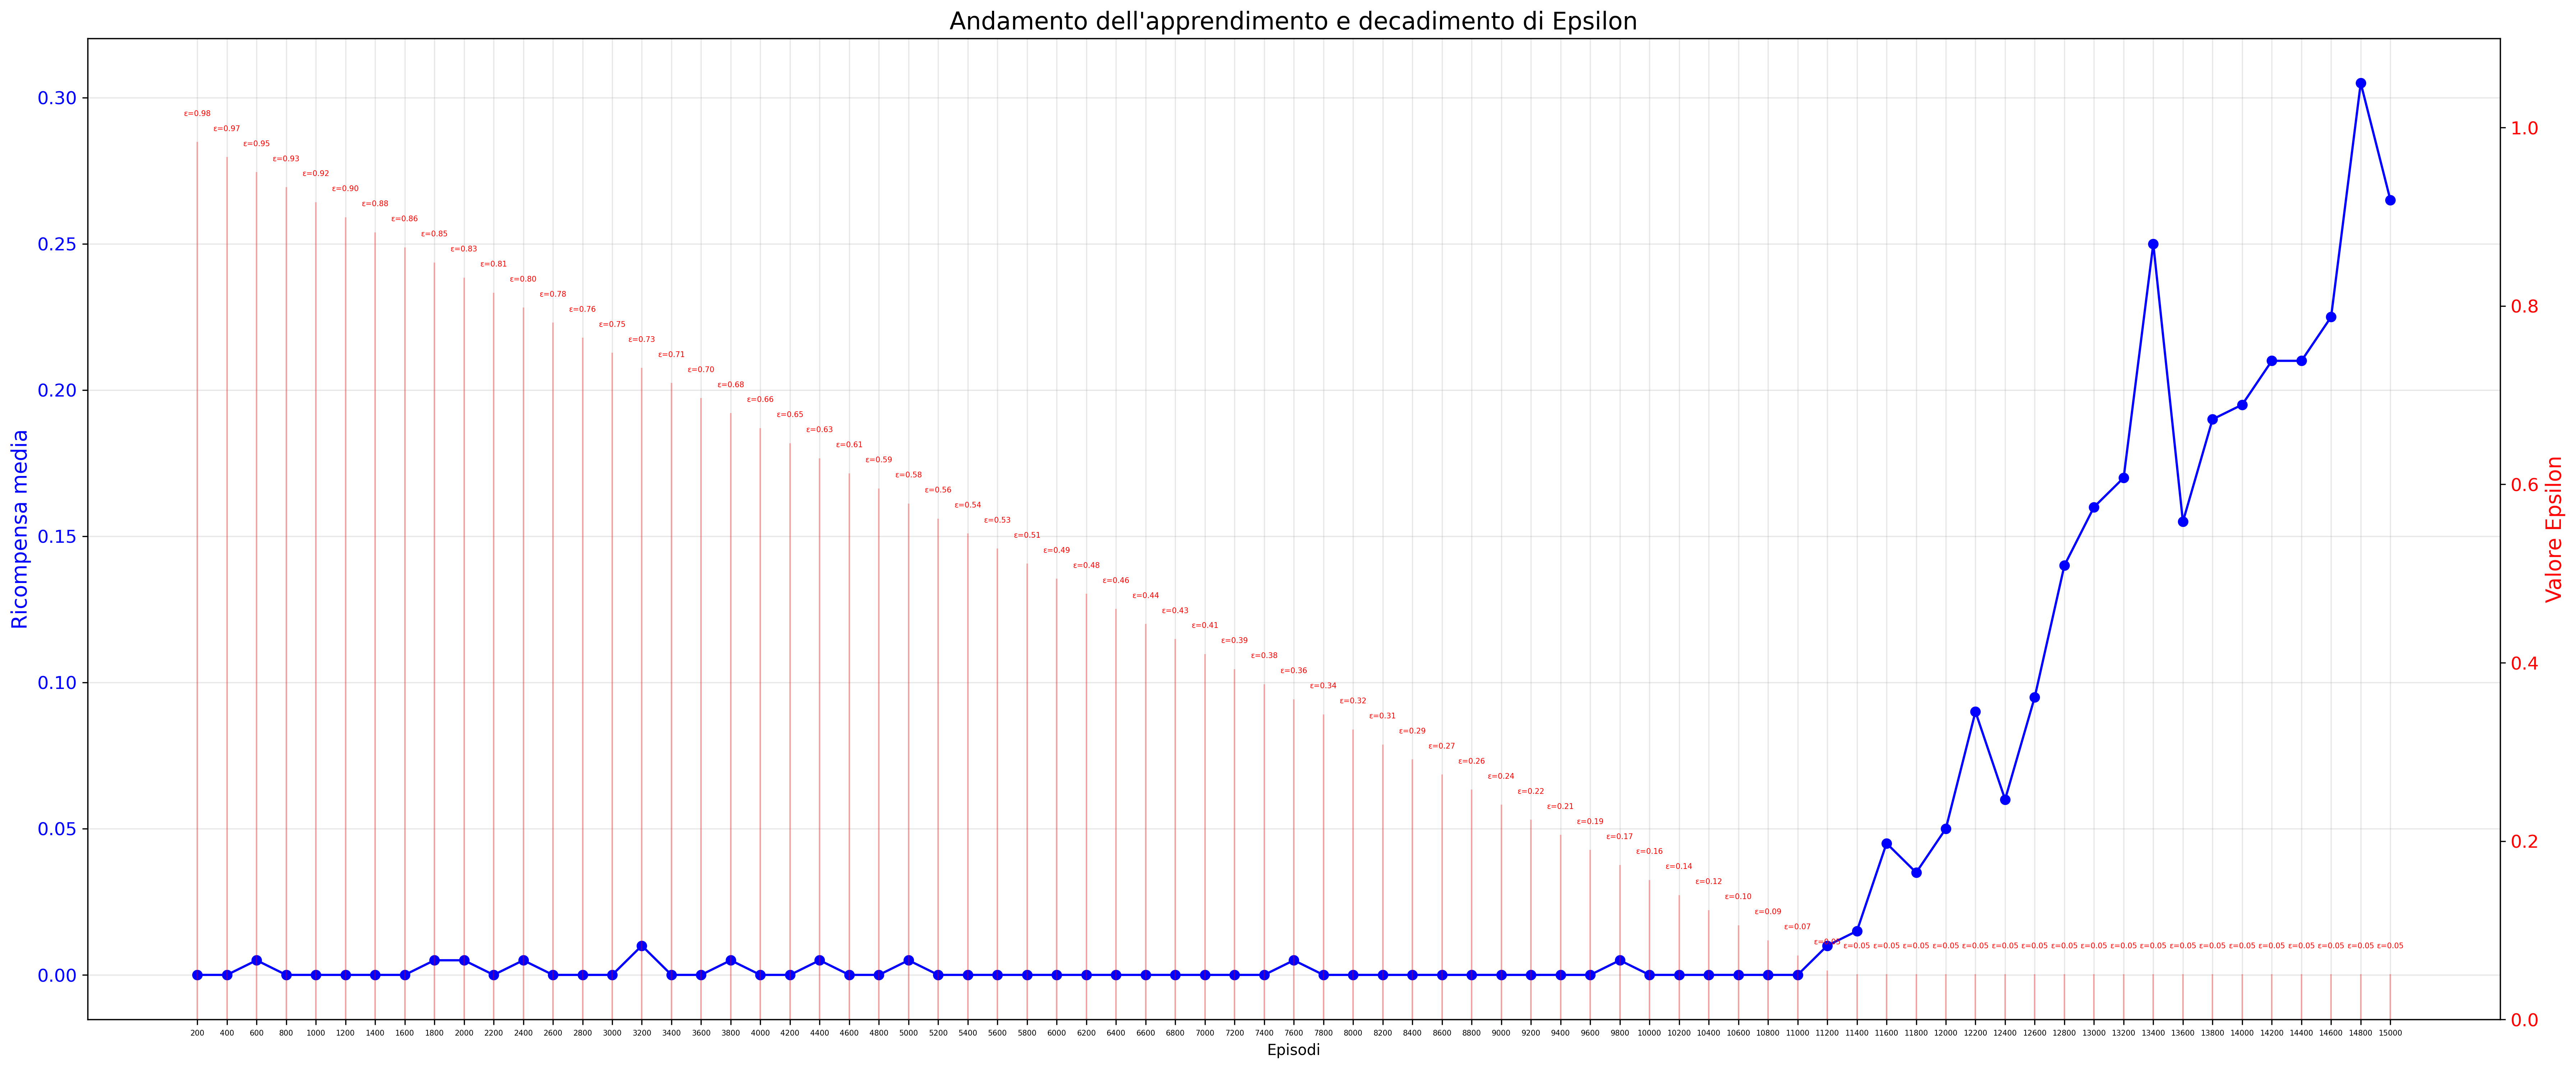
\includegraphics{DQN2;lr=0.01;nep=15000;eps=1.0;fineps=0.05;eps_dec=8.444444444444444e-05;gam=0.99.png}}
\end{center}

\begin{center}
\centering
\resizebox{\textwidth}{!}{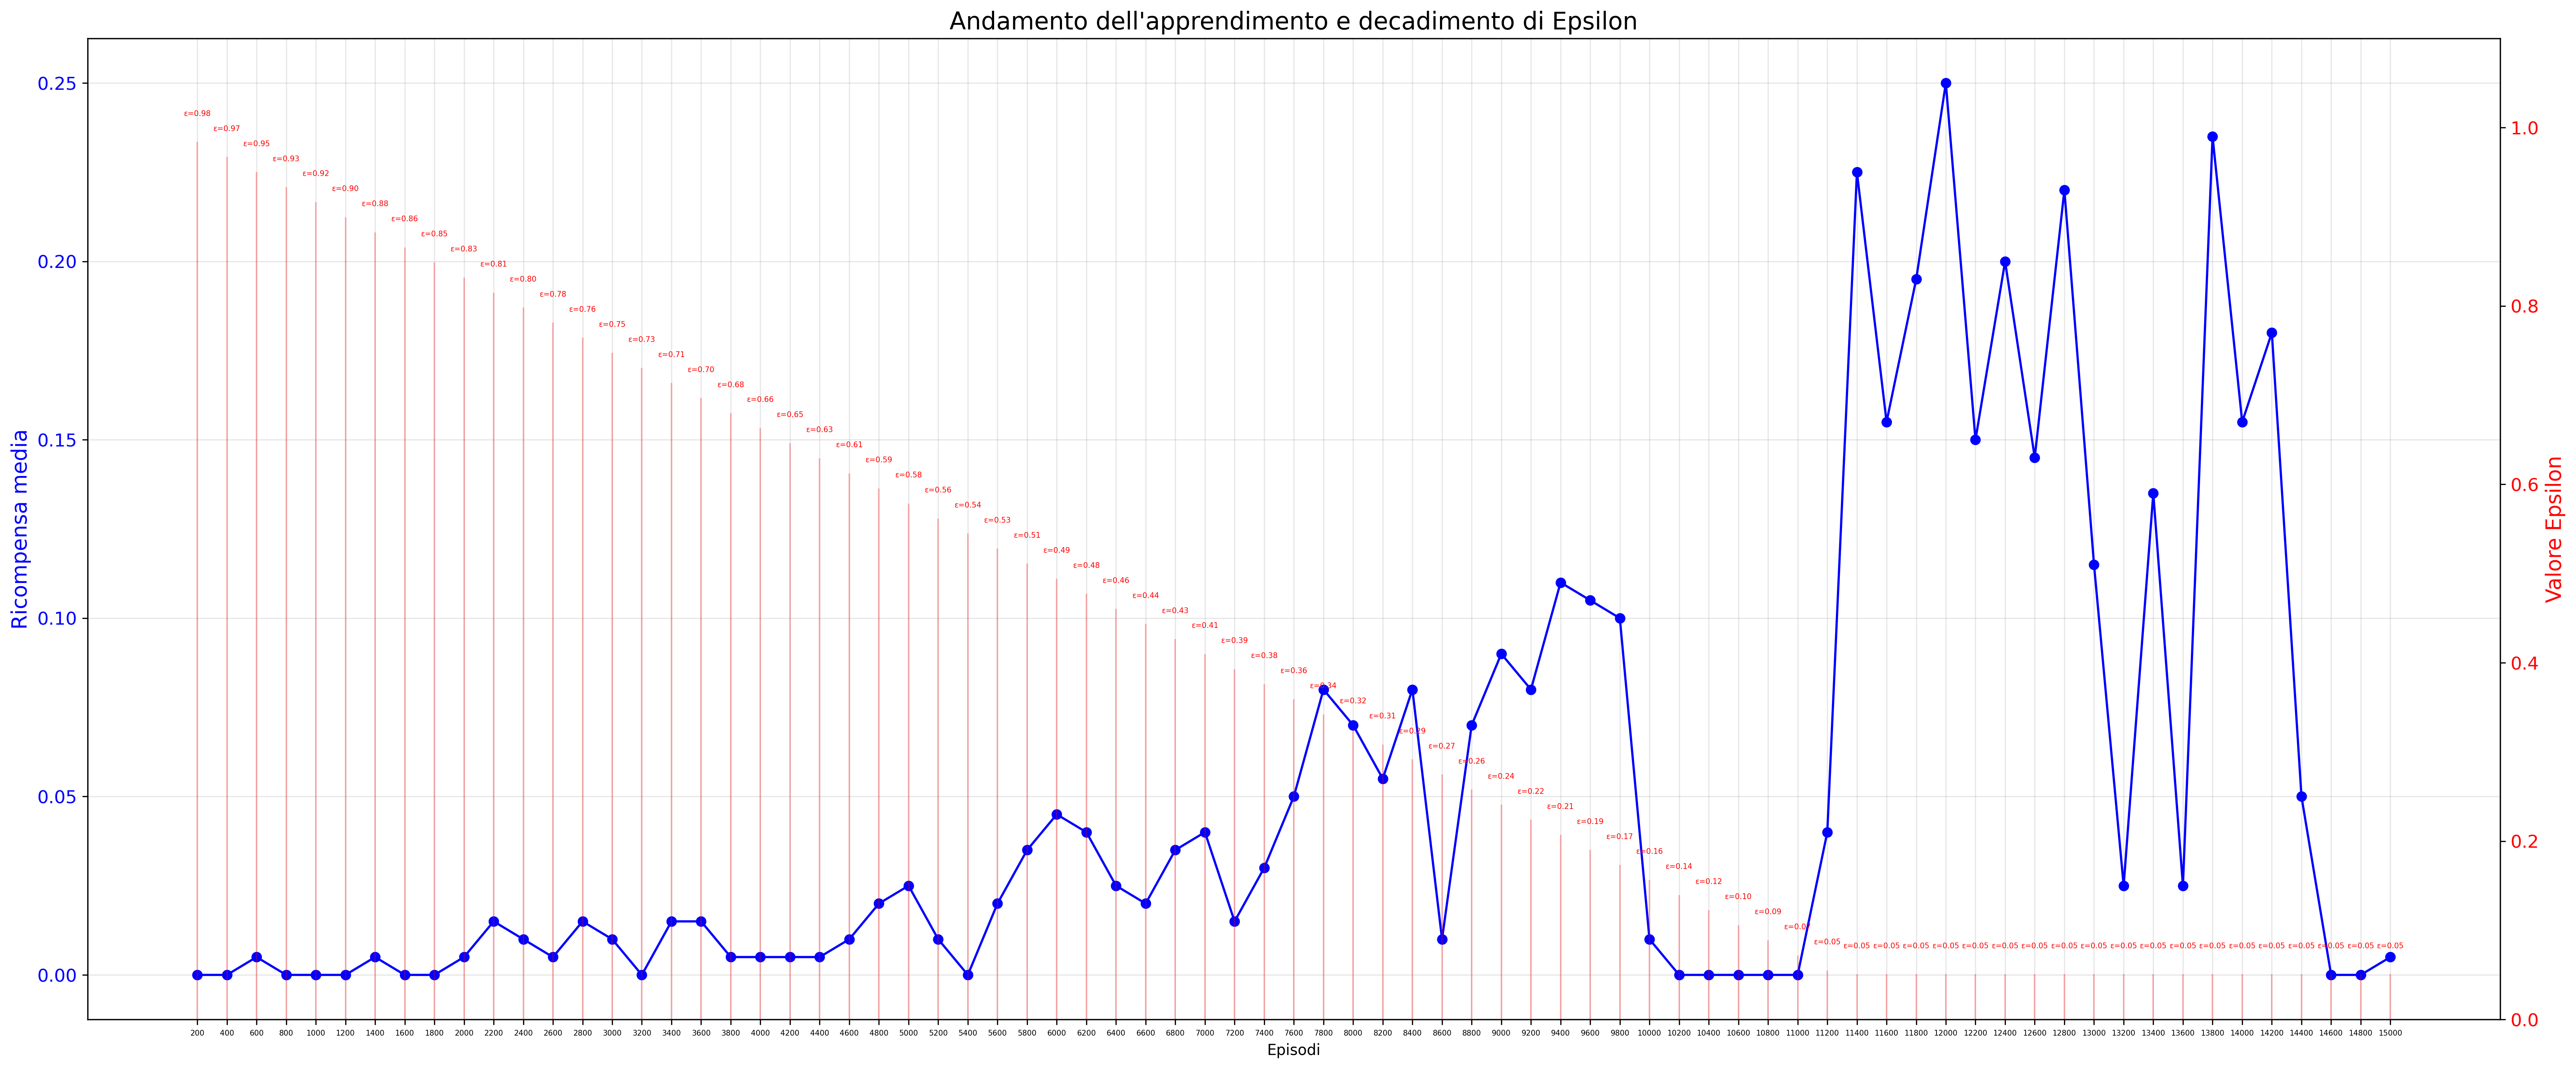
\includegraphics{DQN2;lr=0.001;nep=15000;eps=1.0;fineps=0.05;eps_dec=8.444444444444444e-05;gam=0.99.png}}
\end{center}

\clearpage

In terms of convergence time, the first setting is the only one which converges, and does it near at 11400 episodes.
\\
The second setting, doesn't converge, but at least the average reward increases wrt the episodes, reaching values over 0.25.
\\
Instead, the third configuration has a very strange plot, in which there are two final increasing phases alternated with 2 decreases phases.
\\
With respect to the average cumulative reward at convergence aspect, the first configuration brings a value of 0.27.
\\
After the testing phase, the first setting brings a success rate of the 44.6\%, while the second one of the 40.3\%.
\\
In the end, the third setting brings the worst success rate, which is 0.2\%.
\\
In conclusion, I would say that clearly the first configuration is the best in terms of performance, both in convergence time (which is the only that has it) and in testing average reward.



\subsubsection{Conclusions}

So, in conclusion, I would say that in the case of Deep Q Network in a non deterministic environment, the best configuration found is the following one:

\begin{itemize}
\item[--] $\alpha$= 0.1
\item[--] $\epsilon$ decay= 8.44$\times10^{-5}$
\item[--] initial $\epsilon$ = 1
\item[--] final $\epsilon$ = 0.05
\item[--] gamma = 0.99
\end{itemize}

Having a success rate of 44.6\% and converging in 11400 episodes.


\section{Confrontation between maps}

In conclusion, I would make a brief confrontation between the two used maps, the standard 4x4 and the standard 8x8 ones.
\\
Knowing that the test results in the second part of the report are more accurate (500 episodes vs 2000), we can also draw the following conclusions:
\\
The time needed for the DQN algorithm to execute is almost doubled and this is because of the different number of neurons and links between the 2 neural networks (between their input layers).
\\
Obviously the success rate, over the best found conditions over the DQN algorithm, is very different: 75\% using the map 4x4 and only 45\% for the second map.
\\
Always considering the best found configuration, over the TQL algorithm, the difference is 73\% against a 53\% of success rate.
\\
The last important thing I would notice is about the fact that there are no significant differences between the best success rates between TQL and DQN over the map 4x4: 
\\
and this is because about 75\% is the best result you can have in this stochastic environment, and it was reached in those episodes because of the small state space (only 16 states).
\\
Considering the 8x8 map, is remarked a difference between TQL and DQN, in which the first algorithm performs in a better way (53\% against a 45\%) and, usually, this is a strange result, because should be the opposite.
\\
An explaination to this behaviour could be in the fact that the environment used is pretty simple and discrete, so TQL behaves and the correct way, instead, DQN could, in the best case, reach the TQL performances
\\
but considering its limits due to its approximation of the Q function, done in the training phase.























\end{document}


